%
% main.tex
%

% ===========================================================================
% Dokumenteneinstellungen laden
% ===========================================================================

% Dokumentheader
\documentclass[
	paper = a4,							% A4 Papier
	BCOR10mm,							% Bindekorrektur
%	DIVcalc,							%	DIV-Wert fuer die Erstellung des Satzspiegels, siehe scrguide
	twoside = false,							% Layout f�r einseitigen Druck
  1.4headlines,				% Manuelle Vergr��erung der Kopfzeile. Standardwert 1.25 Zeilen
  openany,             	% Kapitel k�nnen auf geraden und ungeraden Seiten beginnen	
	bibliography=totoc, 	% Literaturverzeichnis ins Inhaltsverzeichnis aufnehmen
	version=first,
	listof=totoc,					% Tabellen- und Abbildungsverzeichnis ins Inhaltsverzeichnis aufnehmen
	index=totoc,					% Index ins Inhaltsverzeichnis aufnehmen
  headinclude,         	% Kopfzeile wird in Seiten-Layouts mit beruecksichtigt
  %footinclude,        	% Fusszeile wird in Seiten-Layouts mit beruecksichtigt
	parskip = half,					% Europ�ischer Satz mit Abstand zwischen Abs�tzen
	chapterprefix = false,   		% "Kapitel" nicht in Kapitl
	fontsize = 12pt,									% Schriftgr��e 12pt                 
	headings = normal,				% kleinere �berschriften
]{scrreprt}

% pers�nliche Daten m�ssen in dem File @"Einstellungen/Labels"  eingetragen werden
%
% Labels.tex
%

% Studentendaten hier eintragen
% =============================

% Name des Betreuers (mit akademischem Titel)
\def \tutor{M.Sc. Fabian Sauter (AP Sensing GmbH)}

% Name des Studenten
\def \student{Swapnil Bhavsar}

% Matrikelnummer des Studenten
\def \studentID{3571387}

% Deutscher Titel der Arbeit
\def \worktitle{Human Movement Detection via Fiber Optical Sensing}

% Englischer Titel der Arbeit
\def \worktitleEnglish{}

% Art der Arbeit
\def \worksubject{Master Thesis} % Bachelorarbeit | Forschungsarbeit | Masterarbeit

\def \worksubjectEnglish{master thesis} % bachelor thesis | research thesis | master thesis

% Startdatum der Arbeit
\def \startdate{December 2024}

% Abgabedatum der Arbeit
\def \submission{June 2025}

% Beginn der Laborarbeit
\def \startLab{Januar 2022}

% Ende der Laborarbeit
\def \endLab{Juni 2022}

% Schlagw�rter der Arbeit
\def \keywords{Delta-Sigma, Modulation, IC-Design,  SiGe}


% PDF Optionen laden, Das Laden dieser Optionen wurde aus der Pr�ambel herausgenommen, da folgender Fehler auftrat: "`tex capacity exceeded save size=5000"'. Die Probleml�sung wird im Internet beschrieben. Knackpunkt: \onehalfspacing (in Pr�ambel) muss nach den pdf Optionen stehen.
% 
% ---------------------------------------------------------------------------
% Pdf Optionen
% ---------------------------------------------------------------------------
%
% Type 1 Fonts f�r bessere darstellung in PDF verwenden.
%
%\usepackage{mathptmx}           % Times + passende Mathefonts
%\usepackage[scaled=.92]{helvet} % skalierte Helvetica als \sfdefault
%\usepackage{courier}            % Courier als \ttdefault


%
% Package f�r Farben im PDF
%
\usepackage{color}
\definecolor{hellgrau}{rgb}{0.9,0.9,0.9}

% Paket f�r Links innerhalb des PDF Dokuments

\definecolor{LinkColor}{rgb}{0,0,0.5}

\definecolor{LinkColor}{rgb}{0,0,0}

% Kapitel, Abbildungen, Tabellen und Literatur verlinken
\usepackage[
	linktocpage,					% Setzt Links in Verzeichnissen auf Seitenzahl --> keine Probleme mit Umbr�chen
	ps2pdf,
	colorlinks=false,			% Links farbig markieren; Druckversion: false, PDF-Version: true
	linkcolor=blue,				% Linkfarbe
	pdftitle={\worktitle},
	pdfauthor={\student},
	pdfsubject={\worksubject, \student},
	pdfkeywords={\keywords}]
{hyperref}


% Anmerkung: Listings sind nicht kompatibel mit 
% Paket um Listings sauber zu formatieren.

\usepackage[savemem]{listings}
\lstloadlanguages{TeX}
\lstloadlanguages{Matlab}


% Listing Definitionen f�r PHP Code

\definecolor{lbcolor}{rgb}{0.85,0.85,0.85}
\lstset{language=[LaTeX]TeX,
	numbers=left,
	stepnumber=1,
	numbersep=5pt,
	numberstyle=\tiny,
	breaklines=true,
	breakautoindent=true,
	postbreak=\space,
	tabsize=2,
	basicstyle=\ttfamily\footnotesize,
	showspaces=false,
	showstringspaces=false,
	extendedchars=true,
	backgroundcolor=\color{lbcolor}}



% Einstellungen des Dokumentes importieren

% ======================
% Einbinden von Packages
% ======================

% Layout
\usepackage{a4}									% Ausgabeformat
\usepackage{lastpage}						% Referenz auf letzte Seite des Dokuments verfügbar
\usepackage{lscape}							% Querformat einer Seite durch den Aufruf \begin{landscape}
\usepackage{rotating}						% Drehen von Gleitobjekten 

% Spracheinstellungen
\usepackage[english]{babel}
   	% neue deutsche Rechtschreibung, deutsche Spracheinstellungen
\usepackage[ansinew]{inputenc}  % direkte Eingabe von Umlauten über Tastatur
\usepackage[T1]{fontenc}				% direkte Eingabe von Umlauten über Tastatur
%\usepackage[utf8]{inputenc}
\usepackage{lmodern}


% Schriften
\usepackage{helvet}         		% Helvetica als serifenlose Schriftart verwenden
\usepackage[bf]{caption}    		% Formatierung von Tabellen- und Bildbeschriftungen
\usepackage{verbatim}						% Ausgabe des Textes wie im Editor dargestellt, Tex-Direktiven werden nicht berücksichtigt
%\setkomafont{sectioning}{\normalfont\bfseries} % Kapitelüberschriften mit Serifen
\setkomafont{sectioning}{\sffamily\bfseries} % Kapitelüberschriften ohne Serifen
\setkomafont{captionlabel}{\normalfont\bfseries}
\setkomafont{descriptionlabel}{\normalfont\bfseries}


% Grafiken
\usepackage{graphics}						% Standardgrafikpaket
\usepackage{graphicx} 					% Erweiterete Grafikoptionen
\usepackage{subfigure}					% Unterabbildungen zulassen
\usepackage{epsfig}							% Einbinden von Grafiken
\usepackage{psfrag}    					% Einfügen von Latex-Schriften in eps-Bilder
\usepackage{svg}
% \usepackage{tikz}								% Package zum Zeichnen von Grafiken
% \usepackage{pgfplots}						% Package zum Zeichnen von Plots, greift auf tikz zu
\usepackage{epstopdf}		% wird nur mit PDFLatex benötigt, damit auch eps-Bilder verwendet werden können

% Paket zum Erweitern der Tabelleneigenschaften
\usepackage{array}							% erweiterte Einstellmöglichkeiten für Spaltenformate
\usepackage{dcolumn}						% Ausrichtung des Dezimalpunktes
\usepackage{multirow}						% mehrere Zeilen zusammefassen
\usepackage{tabularx}   				% Erweiterte Tabellen Optionen
\usepackage{booktabs}						% normgerechte Tabellen
\usepackage{longtable}					% Mehrseitige Tabellen

% Formeln
\usepackage{amsmath}    				% Mathematik-Modus
\usepackage{amsfonts}						% Schriftarten für Mathematik-Modus
% \usepackage{dsfont}							% Zahlenmengen-Schriftart
\usepackage{amssymb}    				% Symbole für Mathematik-Modus
\usepackage{wasysym}						% >>,<<,approx
\usepackage{upgreek}						% nichtkursive griechische Buchstaben
% \usepackage{trfsigns}						% Transformationssymbole

% Aufzählung
\usepackage{mdwlist} 						% Aufzählung unterbrechen mit suspend{enumerate} und resume{enumerate}
\usepackage{paralist}						% Verwendung von unterschiedichen Zeichen in einer Aufzählung


% Sonstiges
\usepackage{ifthen}							% Abfragen und bedingte Formatierung
\usepackage[
  hidelinks,        % remove colored boxes around links
  linktocpage,      % make the page number, not the text, the clickable target
  breaklinks=true,  % allow links to break across lines
]{hyperref}

\usepackage{xspace}    					% für Leerzeichen in Mathe
 
\usepackage{bibgerm}						% Literaturverzeichnis

\usepackage{tikz}		% fuer circuitikz Schaltpläne
\usepackage[european, betterproportions, americaninductors]{circuitikz}

\usepackage{pgfplots}   % um Plots darzustellen          
\pgfplotsset{/pgf/number format/.cd, use comma}  % Komma bei Achsenbeschriftung
\usepgfplotslibrary{groupplots}

% Einheiten
\usepackage{siunitx}  % bei newCommands_user Zeile 21 renewcommand statt newcommand, Zeile 85 auskommentiert
\sisetup{locale = DE} % für Komma statt Punkt
\usepackage{iftex}
\ifPDFTeX
  % pdflatex is in use:
  % Do not load fontspec.
  % Instead, rely on packages like inputenc, fontenc, and lmodern (which you already have)
\else
  % XeLaTeX or LuaLaTeX is in use:
  \usepackage{fontspec}
  % Optionally, set your main font here:
  % \setmainfont{Times New Roman}
\fi
% Core Packages
\usepackage{tikz}          % For TikZ graphics
\usetikzlibrary{positioning, arrows.meta, shapes.geometric, fit}
\usepackage{graphicx}      % For figure handling
\usepackage{xcolor}        % For color shading (e.g., gray!30)
\usepackage[htt]{hyphenat}
% TikZ Libraries
\usetikzlibrary{arrows.meta}
\usepackage{listings}
\lstdefinestyle{pythonstyle}{
    language=Python,
    basicstyle=\footnotesize\ttfamily,
    keywordstyle=\color{blue},
    commentstyle=\color{gray},
    stringstyle=\color{red},
    numbers=left,
    stepnumber=1,
    numbersep=5pt,
    breaklines=true,
    frame=single,
    tabsize=4,
    showstringspaces=false,
}


% ---------------------------------------------------------------------------
% Kopf- und Fu�zeile
% ---------------------------------------------------------------------------

\usepackage[headsepline,plainheadsepline,footsepline,plainfootsepline]{scrlayer-scrpage} 
% Hierbei handelt es sich um ein Paket zur Kontrolle von Kopf- und Fu�zeile.
% N�here Informationen finden sich in der Dokumentation zum KOMA-Skript.

\pagestyle{scrheadings}				% Seitenstil des Pakets scrpage2 laden

% L�schen der voreingestellten Stile
\clearscrheadings							% L�schen des voreingestellten Stils f�r Folgeseiten
\clearscrplain								% L�schen des voreingestellten Stils f�r erste Seite eines Kapitels

% Anordnung der Daten in der Kopfzeile:
% [erste Kapitelseite]{Folgeseiten}
\lohead[\headmark]{\headmark}	% Kapitelname in der Kopfzeile links einf�gen
%\rohead[\pagemark]{\pagemark}	% Seitenzahl in der Kopfzeile rechts einf�gen

% Layout der Fu�zeile laden und setzen
% Erstellung der Fu�zeile in einer Box.
\newsavebox{\footer}


%\ifoot[\usebox{\footer}]{\usebox{\footer}}
\cfoot[\pagemark]{\pagemark}

\automark{chapter}						% automatische Aktualisierung der Kapitel in der Kopfzeile

% Trennlinien
\setheadsepline{.4pt}
\setfootsepline{.4pt} 		% Voreingestellte Trennlinie f�r Fu�zeile ausblenden

\usepackage{setspace}
\onehalfspacing


% neue Befehle importieren
% Floatparameter f�r ein g�nstigeres Platzieren von floatobjekten
\renewcommand{\floatpagefraction}{.75} %default .5
\renewcommand{\textfraction}{.15}
\renewcommand{\topfraction}{.8}
\renewcommand{\bottomfraction}{.5}

% Verschiedene Verweisarten
% Erweiterung zweisprachig, siehe TdS Aufgabensammlung
\iflanguage{ngerman}{
\newcommand{\Equ}[1]{Gleichung~(\ref{equ:#1})}
\newcommand{\Abb}[1]{Abbildung~\ref{fig:#1}}
\newcommand{\abb}[1]{Abb.~\ref{fig:#1}}
\newcommand{\ABB}[2]{Abbildungen~\ref{fig:#1} und~\ref{fig:#2}}
\newcommand{\Abbildungen}[2]{Abbildungen~\ref{fig:#1} bis~\ref{fig:#2}}
\newcommand{\Tab}[1]{Tabelle~\ref{tab:#1}}
\newcommand{\Kap}[1]{Kapitel~\ref{chap:#1}}
\newcommand{\Absch}[1]{Abschnitt~\ref{sec:#1}}
\newcommand{\UAbsch}[1]{Abschnitt~\ref{subsec:#1}}
\newcommand{\App}[1]{Anhang~\ref{app:#1}}
\newcommand{\AppAbsch}[1]{Anhang~\ref{sec:#1}}
% Deutsche Bezeichnungen im Literaturverzeichnis
\newcommand{\btxeditionlong}[1]{Auflage}
}
{
\newcommand{\Equ}[1]{formula~(\ref{equ:#1})}
\newcommand{\Abb}[1]{figure~\ref{fig:#1}}
\newcommand{\abb}[1]{fig.~\ref{fig:#1}}
\newcommand{\ABB}[2]{figure~\ref{fig:#1} and~\ref{fig:#2}}
\newcommand{\Abbildungen}[2]{figures~\ref{fig:#1} to~\ref{fig:#2}}
\newcommand{\Tab}[1]{table~\ref{tab:#1}}
\newcommand{\Kap}[1]{chapter~\ref{chap:#1}}
\newcommand{\Absch}[1]{section~\ref{sec:#1}}
\newcommand{\UAbsch}[1]{section~\ref{subsec:#1}}
\newcommand{\App}[1]{appendix~\ref{app:#1}}
\newcommand{\AppAbsch}[1]{appendix~\ref{sec:#1}}
}

% Tabellenspalten mit Flattersatz setzen, muss \\ vor (z.B.) \raggedright geschuetzt werden:
\newcommand{\PBS}[1]{\let\temp=\\#1\let\\=\temp} 


% Stand: 10.07.2009
% Formatierung in Formeln
\newcommand{\A}[0]{\,\mathrm{A}}															% A-Ampere
\newcommand{\abl}[2]{\frac{\diff{#1}}{\diff{#2}}}							% Ableitung
\newcommand{\Akompl}[0]{\underline{A}}												% A komplex
\newcommand{\const}[0]{\mbox{\it const.}}											% const.
\newcommand{\dB}[0]{\,\mathrm{dB}}														% dB
\newcommand{\dBm}[0]{\,\mathrm{dBm}}													% dBm
\newcommand{\dBDek}[0]{\,\frac{\mathrm{dB}}{\mathrm{Dekade}}}	% dB/Dekade
\newcommand{\diff}[0]{\mathrm{d}}															% Aufrechtes d f�r Differentialoperator
\newcommand{\dt}[0]{\mathrm{\diff}t}													% Aufrechtes d t f�r Differentialoperator
\renewcommand{\Im}[0]{\mathrm{Im}}														% Imagin�rteil
\newcommand{\ind}[1]{_\mathrm{#1}}														% Index aufrecht
\renewcommand{\j}[0]{\mathrm{j}}															% Aufrechtes j f�r imagin�re Einheit
\newcommand{\kompl}[1]{\underline{#1}}												% komplexe Gr��e
\newcommand{\mA}[0]{\,\mathrm{mA}}														% mA
\newcommand{\mS}[0]{\,\mathrm{mS}}														% mA
\newcommand{\ra}[0]{\rightarrow}														  % Pfeil nach rechts
\renewcommand{\Re}[0]{\mathrm{Re}}														% Realteil
\newcommand{\ul}[1]{\underline{#1}}														% Unterstreichung
\renewcommand{\unit}[1]{\,\mathrm{#1}}													% Einheiten aufrecht und Abstand zur Zahl
\newcommand{\Ohm}[0]{\,\mathrm{\Omega}}												% Einheit Ohm
\newcommand{\V}[0]{\,\mathrm{V}}															% V-Volt

% h�ufige Gr��en - Lateinische Buchstaben
\newcommand{\AD}[0]{\underline{A}_{\mathrm{D}}}					% A_D
\newcommand{\CD}[0]{C_{\mathrm{D}}}			 										% C_D
\newcommand{\CDS}[0]{C_{\mathrm{DS}}}		 										% C_DS
\newcommand{\CF}[0]{C_{\mathrm{F}}}											% C_F
\newcommand{\CG}[0]{C_{\mathrm{G}}}			 										% C_G
\newcommand{\CGS}[0]{C_{\mathrm{GS}}}		 										% C_GS
\newcommand{\Cp}[0]{C_{\mathrm{p}}}			 										% C_p
\newcommand{\CPar}[0]{C_{\mathrm{\text{parasit�r}}}}				% C_Par
\newcommand{\Cres}[0]{C_{\mathrm{r}}}												% C_res
\newcommand{\DS}[0]{\Delta\Sigma}														% Delta Sigma
\newcommand{\f}[1]{f_{\mathrm{#1}}}												 	% f_0
\newcommand{\favg}[0]{f_{\mathrm{avg}}}											% f_avg
\newcommand{\fg}[0]{f_{\mathrm{g}}}												 	% f_g
\newcommand{\Fjw}[0]{\underline{F}(\mathrm{j}\omega)}				% F(jw)
\newcommand{\Fkompl}[0]{\underline{F}}										 	% F komplex
\newcommand{\fm}[0]{f_{\mathrm{m}}}													% f_m 
\newcommand{\fN}[0]{f_{\mathrm{N}}}													% f_N 
\newcommand{\fo}[0]{f_{\mathrm{0}}}													% f_o 
\newcommand{\fRes}[0]{f_{\mathrm{Res}}}									% f_Res Aufl�sung
\newcommand{\fs}[0]{f_{\mathrm{s}}}													% f_s 
\newcommand{\fT}[0]{f_{\mathrm{T}}}													% f_T  
\newcommand{\gm}[0]{g_{\mathrm{m}}}												 	% g_m
\newcommand{\Hkompl}[0]{\underline{H}}										 	% H komplex
\newcommand{\iC}[0]{i_{\mathrm{C}}}													% i_C
\newcommand{\IDC}[0]{I_{\mathrm{DC}}}												% I_DC
\newcommand{\IDCI}[0]{I_{\mathrm{DC1}}}											% I_DC1
\newcommand{\IDCII}[0]{I_{\mathrm{DC2}}}										% I_DC2
\newcommand{\iDI}[0]{i_{\mathrm{D1}}}												% i_D1
\newcommand{\iDII}[0]{i_{\mathrm{D2}}}											% i_D2
\newcommand{\iDS}[0]{i_{\mathrm{DS}}}												% i_DS
\newcommand{\Ikompl}[0]{\underline{I}}			 								% I komplex
\newcommand{\iL}[0]{i_{\mathrm{L}}}													% i_L
\newcommand{\Imax}[0]{I_{\mathrm{max}}}											% I_max
\newcommand{\iR}[0]{i_{\mathrm{R}}}													% i_R
\newcommand{\ir}[0]{i_{\mathrm{r}}}													% i_r
\newcommand{\IrI}[0]{I_{\mathrm{r,1}}}											% I_r,1
\newcommand{\irI}[0]{i_{\mathrm{r,1}}}											% i_r,1
\newcommand{\LDS}[0]{L_{\mathrm{DS}}}												% L_DS
\newcommand{\LG}[0]{L_{\mathrm{G}}}			 										% L_G
\newcommand{\Lres}[0]{L_{\mathrm{r}}}												% L_res
\newcommand{\LI}[0]{L_{\mathrm{1}}}													% L_I
\newcommand{\LII}[0]{L_{\mathrm{2}}}												% L_II
\newcommand{\PDC}[0]{P_{\mathrm{DC}}}												% P_DC
\newcommand{\Pout}[0]{P_{\mathrm{out}}}											% P_out
\newcommand{\Poutpk}[0]{P_{\mathrm{out,pk}}}								% P_out,pk
\newcommand{\PVC}[0]{P_{\mathrm{V,C}}}											% P_V,C
\newcommand{\PVG}[0]{P_{\mathrm{V,G}}}											% P_V,G
\newcommand{\PVK}[0]{P_{\mathrm{V,K}}}											% P_V,K
\newcommand{\PVL}[0]{P_{\mathrm{V,L}}}											% P_V,L
\newcommand{\PVR}[0]{P_{\mathrm{V,R}}}											% P_V,R
\newcommand{\PVT}[0]{P_{\mathrm{V,\uptau}}}									% P_V,tau
\newcommand{\RA}[0]{R_{\mathrm{A}}}			 										% R_A
\newcommand{\RDS}[0]{R_{\mathrm{DS}}}												% R_DS
\newcommand{\RDSon}[0]{R_{\mathrm{DS,on}}}									% R_DS,on
\newcommand{\RG}[0]{R_{\mathrm{G}}}			 										% R_G
\newcommand{\RL}[0]{R_{\mathrm{L}}}													% R_L
\newcommand{\Ropt}[0]{R_{\mathrm{opt}}}											% R_opt
\newcommand{\RoptF}[0]{R_{\mathrm{opt,50\ \%}}}							% R_opt,50
\newcommand{\RS}[0]{R_{\mathrm{S}}}													% R_S
%\newcommand{\si}[0]{\mathrm{si}}														% si
\newcommand{\SNR}[0]{\mathrm{SNR}} 													% SNR
\newcommand{\TA}[0]{T_{\mathrm{A}}}													% T_A
\newcommand{\TB}[0]{T_\mathrm{B}} 													% T_B 
\newcommand{\tf}[0]{t_{\mathrm{f}}}													% t_f
\newcommand{\THi}[0]{T_{\mathrm{H}}}												% T_H
\newcommand{\Ti}[0]{T_{\mathrm{i}}}													% T_H
\newcommand{\TLo}[0]{T_{\mathrm{L}}}												% T_L
\newcommand{\tr}[0]{t_{\mathrm{r}}}													% t_r
\newcommand{\TS}[0]{T_{\mathrm{S}}}													% T_S
\newcommand{\To}[0]{T_{\mathrm{0}}}													% T_0
\newcommand{\uAII}[0]{u_{\mathrm{A2}}}											% u_A2
\newcommand{\uAI}[0]{u_{\mathrm{A1}}}												% u_A1
\newcommand{\UBE}[0]{U_{\mathrm{BE}}}												% U_BE
\newcommand{\UC}[0]{\underline{U}_{\mathrm{C}}}							% U_C komplex
\newcommand{\uC}[0]{u_{\mathrm{C}}}													% u_C
\newcommand{\UCC}[0]{U_{\mathrm{CC}}}												% U_CC
\newcommand{\UDC}[0]{U_{\mathrm{DC}}}												% u_DC
\newcommand{\uDI}[0]{u_{\mathrm{D1}}}												% u_D1
\newcommand{\uDII}[0]{u_{\mathrm{D2}}}											% u_D2
\newcommand{\UE}[0]{\underline{U}_{\mathrm{E}}}							% U_E komplex
\newcommand{\Ue}[0]{\underline{U}_{\mathrm{e}}}							% U_e komplex
\newcommand{\UEE}[0]{U_{\mathrm{EE}}}												% U_EE
\newcommand{\uG}[0]{u_{\mathrm{G}}}													% u_G
\newcommand{\UGS}[0]{U_{\mathrm{GS}}}												% U_GS
\newcommand{\uGS}[0]{u_{\mathrm{GS}}}												% u_GS
\newcommand{\UH}[0]{U_{\mathrm{H}}}													% U_H
\newcommand{\UK}[0]{U_{\mathrm{K}}}													% U_K
\newcommand{\Ukompl}[0]{\underline{U}}										 	% U komplex
\newcommand{\uL}[0]{u_{\mathrm{L}}}													% u_L
\newcommand{\Umax}[0]{U_{\mathrm{max}}}											% U_max
\newcommand{\Uout}[0]{U_{\mathrm{out}}}											% U_out
\newcommand{\Uoutpk}[0]{U_{\mathrm{out,pk}}}								% U_out,pk
\newcommand{\uout}[0]{u_{\mathrm{out}}}											% u_out
\newcommand{\uR}[0]{u_{\mathrm{R}}}													% u_R
\newcommand{\URkompl}[0]{\underline{U}_{\mathrm{R}}}			 	% U_R komplex
\newcommand{\Vkompl}[0]{\underline{V}}										 	% V komplex
\newcommand{\Ykompl}[0]{\underline{Y}}											% Y_Zahl komplex
\newcommand{\ZA}[0]{\underline{Z}_{\mathrm{A}}}							% Z_A komplex
\newcommand{\Za}[0]{\underline{Z}_{\mathrm{a}}}							% Z_a komplex
\newcommand{\ZE}[0]{\underline{Z}_{\mathrm{E}}}							% Z_E komplex
\newcommand{\Ze}[0]{\underline{Z}_{\mathrm{e}}}							% Z_e komplex
\newcommand{\Zkompl}[0]{\underline{Z}}										 	% Z komplex
\newcommand{\ZW}[0]{\underline{Z}_{\mathrm{W}}}							% Z_T komplex
\newcommand{\ZT}[0]{\underline{Z}_{\mathrm{T}}}							% Z_T komplex


% Stand: 17.12.2008
% h�ufige Gr��en - Griechische Buchstaben
\newcommand{\etaBP}[0]{\eta_{\mathrm{BP}}}									% eta_BP
\newcommand{\etaC}[0]{\eta_{\mathrm{C}}}										% eta_C
\newcommand{\etaCode}[0]{\eta_{\mathrm{Code}}}							% eta_Code
\newcommand{\etaD}[0]{\eta_{\mathrm{D}}}										% eta_D
\newcommand{\etaK}[0]{\eta_{\mathrm{K}}}										% eta_K
\newcommand{\etaL}[0]{\eta_{\mathrm{L}}}										% eta_L
\newcommand{\etaR}[0]{\eta_{\mathrm{R}}}										% eta_R
\newcommand{\etaRon}[0]{\eta_{\mathrm{R,on}}}								% eta_Ron
\newcommand{\etasim}[0]{\eta_{\mathrm{sim}}}								% eta_sim
\newcommand{\etaT}[0]{\eta_{\mathrm{\uptau}}}								% eta_tau
\newcommand{\w}[1]{\omega_{#1}}															% omega_0
\newcommand{\wg}[0]{\omega_{\mathrm{g}}}										% omega_g


% Stand: 17.12.2008
% Abk�rzungen
\renewcommand{\dh}{\mbox{d.\,h.}\xspace}					% das hei�t / bereits vergeben
\newcommand{\iA}{\mbox{i.\,A.}\xspace}						% im Auftrag
\newcommand{\iAllg}{\mbox{i.\,Allg.}\xspace}			% im Allgemeinen
\newcommand{\ua}{\mbox{u.\,a.}\xspace}						% und andere
\newcommand{\zB}{\mbox{z.\,B.}\xspace}						% zum Beispiel

	
% ====== Definition Spannungs-/Strompfeile ======

% Voltage Arrow between two nodes, arguments:
% positive node, negative node, label pos (left, right, above, below),
% label, (optional: length by which arrow is shortened at each end)
\newcommand{\voltageA}[5][3mm]{
  \draw[->, shorten >= #1, shorten <= #1] (#2) -- (#3) node[midway, #4] {#5} ;
}

% Voltage Arrow next to circuit element, arguments:
% positive node, negative node, label pos, label, half arrow length,
% distance between arrow and circuit element
\newcommand{\voltageB}[6]{
  \coordinate (node_middle) at ($(#1)!0.5!(#2)$);
  \ifthenelse{\equal{#3}{above}}{
    \path (node_middle) + (-#5,#6) coordinate (A+) + (#5,#6) coordinate (A-);
  }{}
  \ifthenelse{\equal{#3}{below}}{
    \path (node_middle) + (-#5,-#6) coordinate (A+) + (#5,-#6) coordinate (A-);
  }{}
  \ifthenelse{\equal{#3}{left}}{
    \path (node_middle) + (-#6,#5) coordinate (A+) + (-#6,-#5) coordinate (A-);
  }{}
  \ifthenelse{\equal{#3}{right}}{
    \path (node_middle) + (#6,#5) coordinate (A+) + (#6,-#5) coordinate (A-);
  }{}
  \draw[->] (A+) -- (A-) node[midway, #3] {#4};
}

% Current Arrow next to a given node, arguments:
% node, label pos, label, length of arrow, distance arrow/wire,
% length of shift parallel to wire
\newcommand{\currentA}[6]{
  \ifthenelse{\equal{#2}{above}}{
    \path (#1) ++ (#6,#5) coordinate (A+) ++ (#4,0) coordinate (A-);
  }{}
  \ifthenelse{\equal{#2}{below}}{
    \path (#1) ++ (#6,-#5) coordinate (A+) ++ (#4,0) coordinate (A-);
  }{}
  \ifthenelse{\equal{#2}{left}}{
    \path (#1) ++ (-#5,-#6) coordinate (A+) ++ (0,-#4) coordinate (A-);
  }{}
  \ifthenelse{\equal{#2}{right}}{
    \path (#1) ++ (#5,-#6) coordinate (A+) ++ (0,-#4) coordinate (A-);
  }{}
  \draw[->] (A+) -- (A-) node[midway, #2] {#3};
}




% H�ufig verwendetet Ersetzungen in EPS-Grafiken	
	
	\newcommand{\psfragEinheiten}{
			\psfrag{dB}{$\unit{dB}$}
			\psfrag{V}{$\unit{dB}$}
			\psfrag{ns}{$\unit{ns}$}
			\psfrag{ps}{$\unit{ps}$}
			\psfrag{mA}{$\unit{mA}$}
			\psfrag{A}{$\unit{A}$}
			\psfrag{Hz}{$\unit{Hz}$}
			\psfrag{kHz}{$\unit{kHz}$}
			\psfrag{MHz}{$\unit{MHz}$}
			\psfrag{GHz}{$\unit{GHz}$}
	}
	\newcommand{\psfragNormFreq}{
			\psfrag{0.0}{0.0}
			\psfrag{0.05}{0.05}
			\psfrag{0.1}{0.1}
			\psfrag{0.15}{0.15}
			\psfrag{0.2}{0.2}
			\psfrag{0.25}{0.25}
			\psfrag{0.3}{0.3}
			\psfrag{0.35}{0.35}
			\psfrag{0.4}{0.4}
			\psfrag{0.45}{0.45}
			\psfrag{0.5}{0.5}
	}
	
\newcommand{\psfragNegNumbers}{
			\psfrag{-1}{-1}
			\psfrag{-2}{-2}
			\psfrag{-3}{-3}
			\psfrag{-4}{-4}
			\psfrag{-5}{-5}
			\psfrag{-6}{-6}
			\psfrag{-7}{-7}
			\psfrag{-8}{-8}
			\psfrag{-9}{-9}
			\psfrag{-10}{-10}
			\psfrag{-11}{-11}
			\psfrag{-12}{-12}
			\psfrag{-13}{-13}
			\psfrag{-14}{-14}
			\psfrag{-15}{-15}
			\psfrag{-20}{-20}
			\psfrag{-25}{-25}
			\psfrag{-30}{-30}
			\psfrag{-35}{-35}
			\psfrag{-40}{-40}
			\psfrag{-45}{-45}
			\psfrag{-50}{-50}
			\psfrag{-55}{-55}
			\psfrag{-60}{-60}
			\psfrag{-65}{-65}
			\psfrag{-70}{-70}
			\psfrag{-75}{-75}
			\psfrag{-80}{-80}
			\psfrag{-85}{-85}
			\psfrag{-90}{-90}
			\psfrag{-95}{-95}
			\psfrag{-100}{-100}			
			}

\newcommand{\psfragPosNumbers}{			
			\psfrag{0}{0}
			\psfrag{1}{1}
			\psfrag{2}{2}
			\psfrag{3}{3}
			\psfrag{4}{4}
			\psfrag{5}{5}
			\psfrag{6}{6}
			\psfrag{7}{7}
			\psfrag{8}{8}
			\psfrag{9}{9}
			\psfrag{10}{10}
			\psfrag{11}{11}
			\psfrag{12}{12}
			\psfrag{13}{13}
			\psfrag{14}{14}
			\psfrag{15}{15}
			\psfrag{20}{20}
			\psfrag{25}{25}
			\psfrag{30}{30}
			\psfrag{35}{35}
			\psfrag{40}{40}
			\psfrag{45}{45}
			\psfrag{50}{50}
			\psfrag{55}{55}
			\psfrag{60}{60}
			\psfrag{65}{65}
			\psfrag{70}{70}
			\psfrag{75}{75}
			\psfrag{80}{80}
			\psfrag{85}{85}
			\psfrag{90}{90}			
			\psfrag{95}{95}
			\psfrag{100}{100}
		}

\newcommand{\psfragNegNumbersSmall}{		
			\psfrag{-1}{\footnotesize -1}
			\psfrag{-2}{\footnotesize -2}
			\psfrag{-3}{\footnotesize -3}
			\psfrag{-4}{\footnotesize -4}
			\psfrag{-5}{\footnotesize -5}
			\psfrag{-6}{\footnotesize -6}
			\psfrag{-7}{\footnotesize -7}
			\psfrag{-8}{\footnotesize -8}
			\psfrag{-9}{\footnotesize -9}
			\psfrag{-10}{\footnotesize -10}
			\psfrag{-11}{\footnotesize -11}
			\psfrag{-12}{\footnotesize -12}
			\psfrag{-13}{\footnotesize -13}
			\psfrag{-14}{\footnotesize -14}
			\psfrag{-15}{\footnotesize -15}
			\psfrag{-20}{\footnotesize -20}
			\psfrag{-25}{\footnotesize -25}
			\psfrag{-30}{\footnotesize -30}
			\psfrag{-35}{\footnotesize -35}
			\psfrag{-40}{\footnotesize -40}
			\psfrag{-45}{\footnotesize -45}
			\psfrag{-50}{\footnotesize -50}
			\psfrag{-55}{\footnotesize -55}
			\psfrag{-60}{\footnotesize -60}
			\psfrag{-65}{\footnotesize -65}
			\psfrag{-70}{\footnotesize -70}
			\psfrag{-75}{\footnotesize -75}
			\psfrag{-80}{\footnotesize -80}
			\psfrag{-85}{\footnotesize -85}
			\psfrag{-90}{\footnotesize -90}
			\psfrag{-95}{\footnotesize -95}
			\psfrag{-100}{\footnotesize -100}
}	
\newcommand{\psfragPosNumbersSmall}{		
			\psfrag{0}{\footnotesize 0}
			\psfrag{1}{\footnotesize 1}
			\psfrag{2}{\footnotesize 2}
			\psfrag{3}{\footnotesize 3}
			\psfrag{4}{\footnotesize 4}
			\psfrag{5}{\footnotesize 5}
			\psfrag{6}{\footnotesize 6}
			\psfrag{7}{\footnotesize 7}
			\psfrag{8}{\footnotesize 8}
			\psfrag{9}{\footnotesize 9}
			\psfrag{10}{\footnotesize 10}
			\psfrag{11}{\footnotesize 11}
			\psfrag{12}{\footnotesize 12}
			\psfrag{13}{\footnotesize 13}
			\psfrag{14}{\footnotesize 14}
			\psfrag{15}{\footnotesize 15}
			\psfrag{20}{\footnotesize 20}
			\psfrag{25}{\footnotesize 25}
			\psfrag{30}{\footnotesize 30}
			\psfrag{35}{\footnotesize 35}
			\psfrag{40}{\footnotesize 40}
			\psfrag{45}{\footnotesize 45}
			\psfrag{50}{\footnotesize 50}
			\psfrag{55}{\footnotesize 55}
			\psfrag{60}{\footnotesize 60}
			\psfrag{65}{\footnotesize 65}
			\psfrag{70}{\footnotesize 70}
			\psfrag{75}{\footnotesize 75}
			\psfrag{80}{\footnotesize 80}
			\psfrag{85}{\footnotesize 85}
			\psfrag{90}{\footnotesize 90}			
			\psfrag{95}{\footnotesize 95}
			\psfrag{100}{\footnotesize 100}			
			}						% Laden h�ufiger Abk�rzungen  in EPS Grafiken

% Trennungsregeln laden
%
% Trennungsliste.tex
%

% Erg�nzung der Regeln zur Silbentrennung
% =======================================

% Erg�nzungen in dieser Liste bitte auch in der Vorlage mitf�hren.

\hyphenation{Aus-gangs-sig-nal}
\hyphenation{Aus-gangs-sig-nals}
\hyphenation{Chip-her-stel-ler}
\hyphenation{dif-fe-ren-tiell}
\hyphenation{dif-fe-ren-tiel-len}
\hyphenation{Ein-gangs-sig-nal}
\hyphenation{Ein-gangs-sig-nals}
\hyphenation{Ein-gangs-wi-der-stand}
\hyphenation{Ein-gangs-wi-der-stands}
\hyphenation{Im-puls-ant-wort}
\hyphenation{Im-puls-ant-wor-ten}
\hyphenation{Li-nien}
\hyphenation{Li-nien-spek-trum}
\hyphenation{Lo-gik-sig-na-len}
\hyphenation{Lo-gik-sig-nal}
\hyphenation{Lo-gik-sig-nals}
\hyphenation{Schal-tung}
\hyphenation{Sig-nal}
\hyphenation{Sig-nals}
\hyphenation{Sig-nalen}
\hyphenation{Sig-nal-mo-dell}
\hyphenation{Sig-nal-mo-dells}
\hyphenation{Sig-nal-ge-ne-ra-tor}
\hyphenation{Sig-nal-ge-ne-ra-to-ren}
\hyphenation{Sig-nal-ge-ne-ra-tors}
\hyphenation{Si-mu-la-tion}
\hyphenation{Rausch-ver-h�lt-nis}
\hyphenation{Trans-im-pe-danz-ver-st�r-ker}
\hyphenation{vo-raus}


% ===========================================================================
% Beginn des Dokumentes
% ===========================================================================
\begin{document}


% ---------------------------------------------------------------------------
% Titelseite, Verzeichnisse 
% ---------------------------------------------------------------------------

% r�mische Nummerierung der Seiten f�r die Verzeichnisse
\pagenumbering{Roman}

% Titelseite
%
% Titel-tex
%

% Die vertikalen Abst�nde nach Eingabe der Daten bitte selbst anpassen.

\begin{titlepage}
	\begin{minipage}{0.55\linewidth}
		\textsc{Institute of Electrical  \\
			and Optical Communications \\
			Prof. Dr.-Ing. Georg Rademacher}
	\end{minipage}
	\begin{minipage}{0.5\linewidth}
		\hfill 
\includegraphics[height=1.4cm]{Bilder/eps/unistuttgart_logo_deutsch_cmyk}

	\end{minipage}

	
	\begin{center}															% zentriert
		
		\vspace{25mm}														% vertikaler Abstand


		\begin{LARGE}
			\textsf{\textbf{\worktitle}}
		\end{LARGE}

		\vspace{7mm}														% vertikaler Abstand

		\begin{large}
			\textsf{\textbf{\worktitleEnglish}}
		\end{large}

		\vspace{10mm}														% vertikaler Abstand

		\textsf{\textbf{\worksubject}}
		
		\textsf{\textbf{Submitted at University of Stuttgart}}

		\vspace{7mm}														% vertikaler Abstand

		\textsf{\textbf{\student}}

		\vspace{15mm}														% vertikaler Abstand

		\textsf{\textbf{Supervisor: \tutor}}

		\vfill																% vertikaler Abstand
		
  	\begin{minipage}[t]{.8\textwidth}										% Unterseite einf�gen
	  	\begin{tabular}[h]{l l}												% Tabelle mit 2 linksb. Spalten
				Start of Thesis: & \startdate \\
				%Beginn der Laborarbeit: &	\startLab \\
				%Ende der Laborarbeit: & \endLab \\
				End of Thesis: & \submission 
  	 	\end{tabular}
		\end{minipage}    
	\end{center}

\end{titlepage}
 % Titelseite f�r studentische Arbeiten

% Seitennummerierung auf der zweiten Seite beginnen
\setcounter{page}{1}

% Zusammenfassung in deutscher und englischer Sprache
%
% Zusammenfassung.tex
%

% =========================================
% Zusammenfassung
% =========================================

% Die �berschriften der Zusammenfassung und des Abstract werden
% nicht als \chapter angelegt, sondern lediglich als gro�er,
% fettgedruckter Text. Dadurch wird zum einen verhindert, dass
% die Zusammenfassung ins Inhaltsverzeichnis aufgenommen wird,
% zum anderen wird die Seite besser ausgenutzt (Zusammenfassung
% und Abstract sollten eine Seite nicht �bersteigen).

%\addchap{Zusammenfassung}

					% Leerraum zwischen Zusammenfassung und Abstract

% Englische �bersetzung der Zusammenfassung

\begin{Large}
\textsf{\textbf{Abstract}}\\
\end{Large}


Perimeter monitoring is a cornerstone of security and surveillance. Distributed Acoustic Sensing (DAS) turns miles of optical fiber into a continuous, high-resolution microphone that captures tiny ground vibrations in real time. With recent developments in machine learning, never before seen new possibilities emerged to train models detecting and distinguishing between individual human activities based on DAS phase data. In this work, we present the spectrogram classifier framework developed in collaboration with AP Sensing to detect and distinguish various walking patterns and footsteps from DAS data. First, it transforms the raw DAS phase data into  time frequency images (spectrograms), then feeds them into two modern vision networks: ConvNeXt V2 and EfficientNet. We train both ConvNeXt V2 and EfficientNet on two distinct dataset configurations: a single-channel stream sampled over 1.728 seconds, and a ten-channel stream sampled over 2 seconds yielding four total model-dataset combinations for direct performance comparison. On the ten-channel recordings, both models top 99\% accuracy and produce almost no false alarms. By contrast, the one-channel setup drops to about 88\% accuracy and fires off many more spurious alerts. This clear gap shows that giving the model a richer spatial picture (ten channels) dramatically boosts reliability. By combining GPU-accelerated preprocessing with these proven backbones, our pipeline moves from a lab prototype to a field-ready perimeter-monitoring tool.





% Inhaltsverzeichnis
\tableofcontents

% Abk�rzungen und Formelzeichen

\addchap{Abbreviation}

% Große fette Überschrift
{\Large\textbf{Abbreviation}}

% Abkürzungsverzeichnis im longtable-Format
\vspace{0mm}
\setlength\LTleft{0pt}
\setlength\LTright{0pt}

\begin{longtable}{l @{\extracolsep\fill} p{0.8\textwidth}}
  \toprule
  {\itshape Abbreviation} & {\itshape Meaning}\\
  \midrule
  API    & Application Programming Interface\\
  C-OTDR & Coherent Optical Time Domain Refractometry\\
  CNN    & Convolutional Neural Network\\
  DAS    & Digital Acoustic Sensing\\
  DTGS   & Distributed Temperature Gradient Sensing\\
  DPU    & Digital Processing Unit\\
  EDFA   & Erbium-Doped Fiber Amplifier\\
  FBE    & Frequency Band Energy\\
  FIFO   & First-In First-Out\\
  GPU    & Graphics Processing Unit\\
  HDF5   & Hierarchical Data Format version 5\\
  I/O    & Input/Output\\
  IP     & Internet Protocol\\
  IU     & Interrogator Unit\\
  JSON   & JavaScript Object Notation\\
  ML     & Machine Learning\\
  RNN    & Recurrent Neural Network\\
  RGB    & Red Green Blue\\
  STFT   & Short Time Fourier Transform\\
  SSD    & Solid State Drive\\
  USB    & Universal Serial Bus\\
  \bottomrule
\end{longtable}




% Abbildungsverzeichnis
% wird normalerweise nicht verwendet
\cleardoublepage
\listoffigures


%	Tabellenverzeichnis
% wird normalerweise nicht verwendet
\cleardoublepage
\lstlistoflistings


% Aufgabenstellung



% ---------------------------------------------------------------------------
%	Hauptteil
% ---------------------------------------------------------------------------
% arabische Numerrierung der Seiten des Hauptteils
\pagenumbering{arabic}
\setcounter{page}{1}

% Kapitel einbinden
%
% Kapitel1.tex 
%
\chapter{Introduction}

Perimeter monitoring is a cornerstone of modern security and surveillance of a location. A powerful technology for this application is Digital Acoustic Sensing (DAS)~\cite{duckworth}, which effectively transforms long stretches of fibre optic cable into a continuous array of highly sensitive microphones. These systems capture detailed acoustic data by measuring minute phase shifts in light traveling through the fibre, enabling the real-time detection of ground vibrations caused by various activities.

This thesis focuses on activities relevant to perimeter security, such as walking, climbing, or vehicle movement, as conceptually illustrated in the theoretical airport security layout in Figure~\ref{Airport}. In such a scenario, a DAS system, with fiber optic cables indicated by the red lines, would be deployed to monitor the entire perimeter for potential intrusions.

\begin{figure}[h]
    \centering
    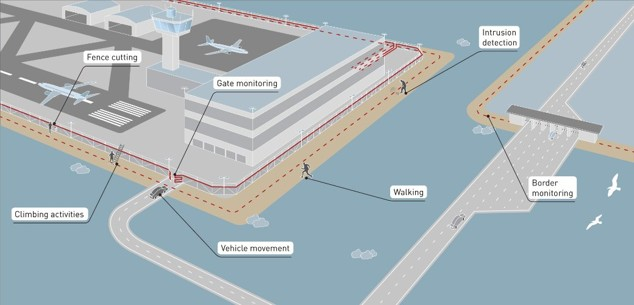
\includegraphics[width=\linewidth]{Bilder/jpg/Airport.jpg}
    \caption{A theoretical perimeter monitoring setup at an airport~\cite{Airport_Image}.}
    \label{Airport}
\end{figure}

While DAS provides a wealth of raw data, interpreting this data to reliably identify specific events is a significant challenge. To address this, this thesis presents the spectrogram classifier framework, a complete pipeline designed to detect and classify human footsteps from raw DAS phase data. The research presented was conducted in collaboration with AP Sensing, who provided the DAS system (Figure~\ref{System}) and associated software used for data acquisition.

The core of the framework first transforms raw, one-dimensional DAS phase data into two-dimensional time-frequency representations called spectrograms. These spectrograms, which visually resemble images, are then fed into modern deep learning vision networks for classification. This approach leverages the advanced pattern-recognition capabilities of convolutional neural networks (CNNs) to distinguish between ambient noise and the unique signatures of footsteps.

\begin{figure}[h]
    \centering
    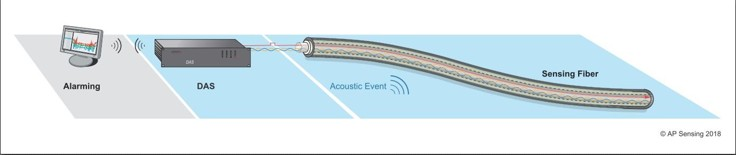
\includegraphics[width=\linewidth]{Bilder/jpg/System.jpg}
    \caption{DAS setup~\cite{DAS_PPT}.}
    \label{System}
\end{figure}

To validate the framework and determine the most effective configuration, this thesis evaluates two state-of-the-art vision models: ConvNeXt V2~\cite{liu2023convnextv2} and EfficientNet~\cite{tan2019efficientnet}. The performance of these models is rigorously tested by training and evaluating them on a custom dataset of walking patterns. By comparing their accuracy, false alarm rates, and real-time performance, this work identifies the optimal model and data configuration for a field-ready perimeter monitoring tool. Ultimately, this thesis demonstrates the efficacy of the Spectrogram Classifier Framework as a robust and reliable solution for security surveillance applications.
%
% Kapitel2.tex
%
%
\chapter{Background}
This chapter details the principles of Distributed Acoustic Sensing (DAS), including the C-OTDR measurement principle, the components of the AP Sensing DAS hardware, and the functionality of the DAS Configurator application used for data acquisition and visualization. Then, it introduces the fundamentals of Machine Learning for image recognition, explaining key evaluation metrics derived from the confusion matrix, data augmentation techniques, and the basics of the PyTorch and Kornia libraries. The chapter concludes with a literature review that situates this work within the context of previous research on DAS-based activity detection.

\section{Distributed Acoustic Sensing}

Distributed Acoustic Sensing (DAS) transforms a standard fiber-optic cable into a dense array of thousands of virtual microphones. By sending pulses of laser light down the fiber and analyzing the coherent Rayleigh backscatter, a DAS system can detect minute physical disturbances acoustic vibrations or strain at any point along the cable's length. This enables precise localization and real-time monitoring of events over distances of several kilometers. Common applications include power-cable integrity checks, pipeline leak detection, train tracking, and perimeter security, where the system can continuously surveil and trigger alarms for anomalous activity. 

\subsection{Measurement Principle}

The current measuring principle behind the DAS is measurement of acoustic vibrations based on the Coherent Optical Time Domain Refractometry (C-OTDR). It measures the change in length and index of refraction of the fiber induced by the temperature changes and acoustic or seismic waves interacting with the cable~\cite{duckworth}. Laser is sent into the fiber and the backscattered light is detected and analyzed. 

\begin{figure}[h]
    \centering
    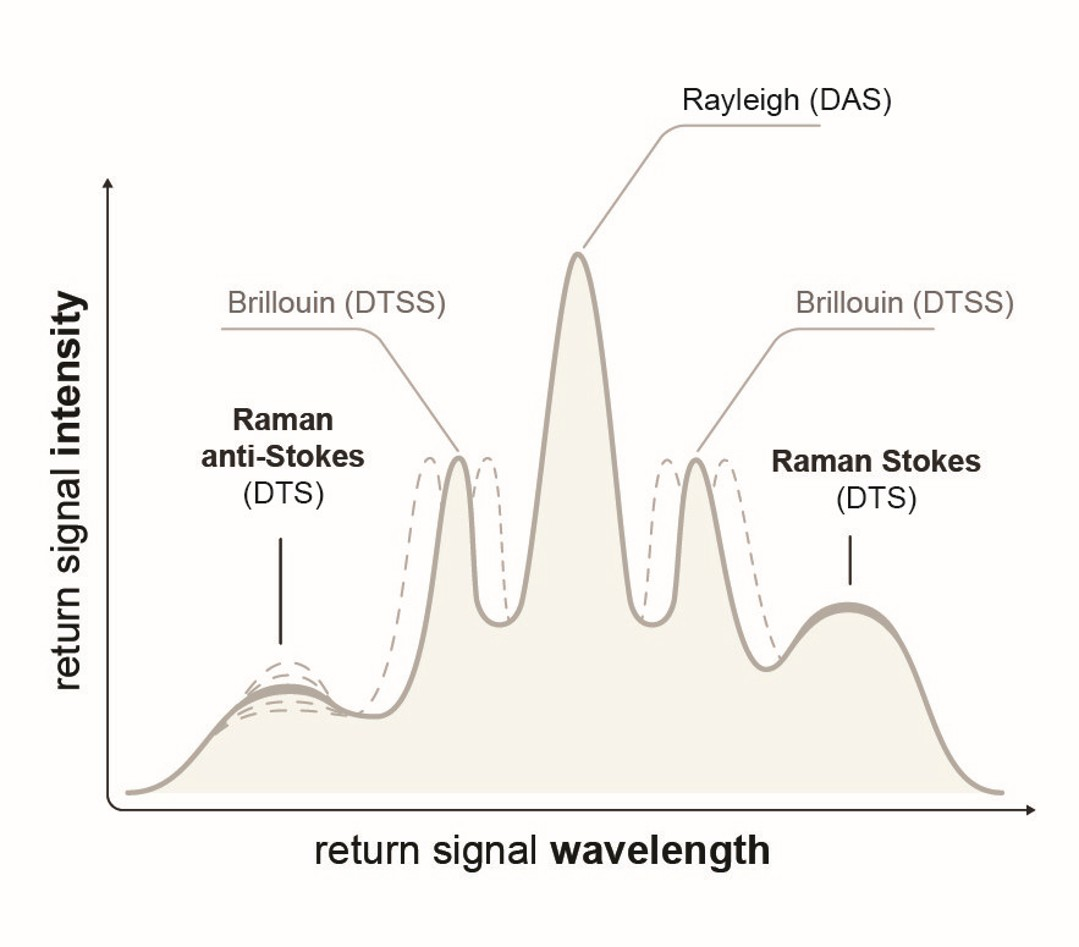
\includegraphics[width=0.7\linewidth]{Bilder/jpg/COTDR.jpg}
    \caption{Spectral signal intensity distribution of the backscattered light~\cite{DAS_Manual}}
    \label{COTDR}
\end{figure}
 
Spectral signal intensity distribution of the backscattered light from the fiber is shown in Figure~\ref{COTDR}. DAS systems work on the Rayleigh Backscattering which is the highest peak in the Figure. It is a small fraction of light scattered by microscopic variations in fibre's refractive index. By sending the short pulses of laser and measuring the backscattering Rayleigh signal as a function of time, signals are localized along the fiber~\cite{masoudi}.  

\begin{figure}[h]
    \centering
    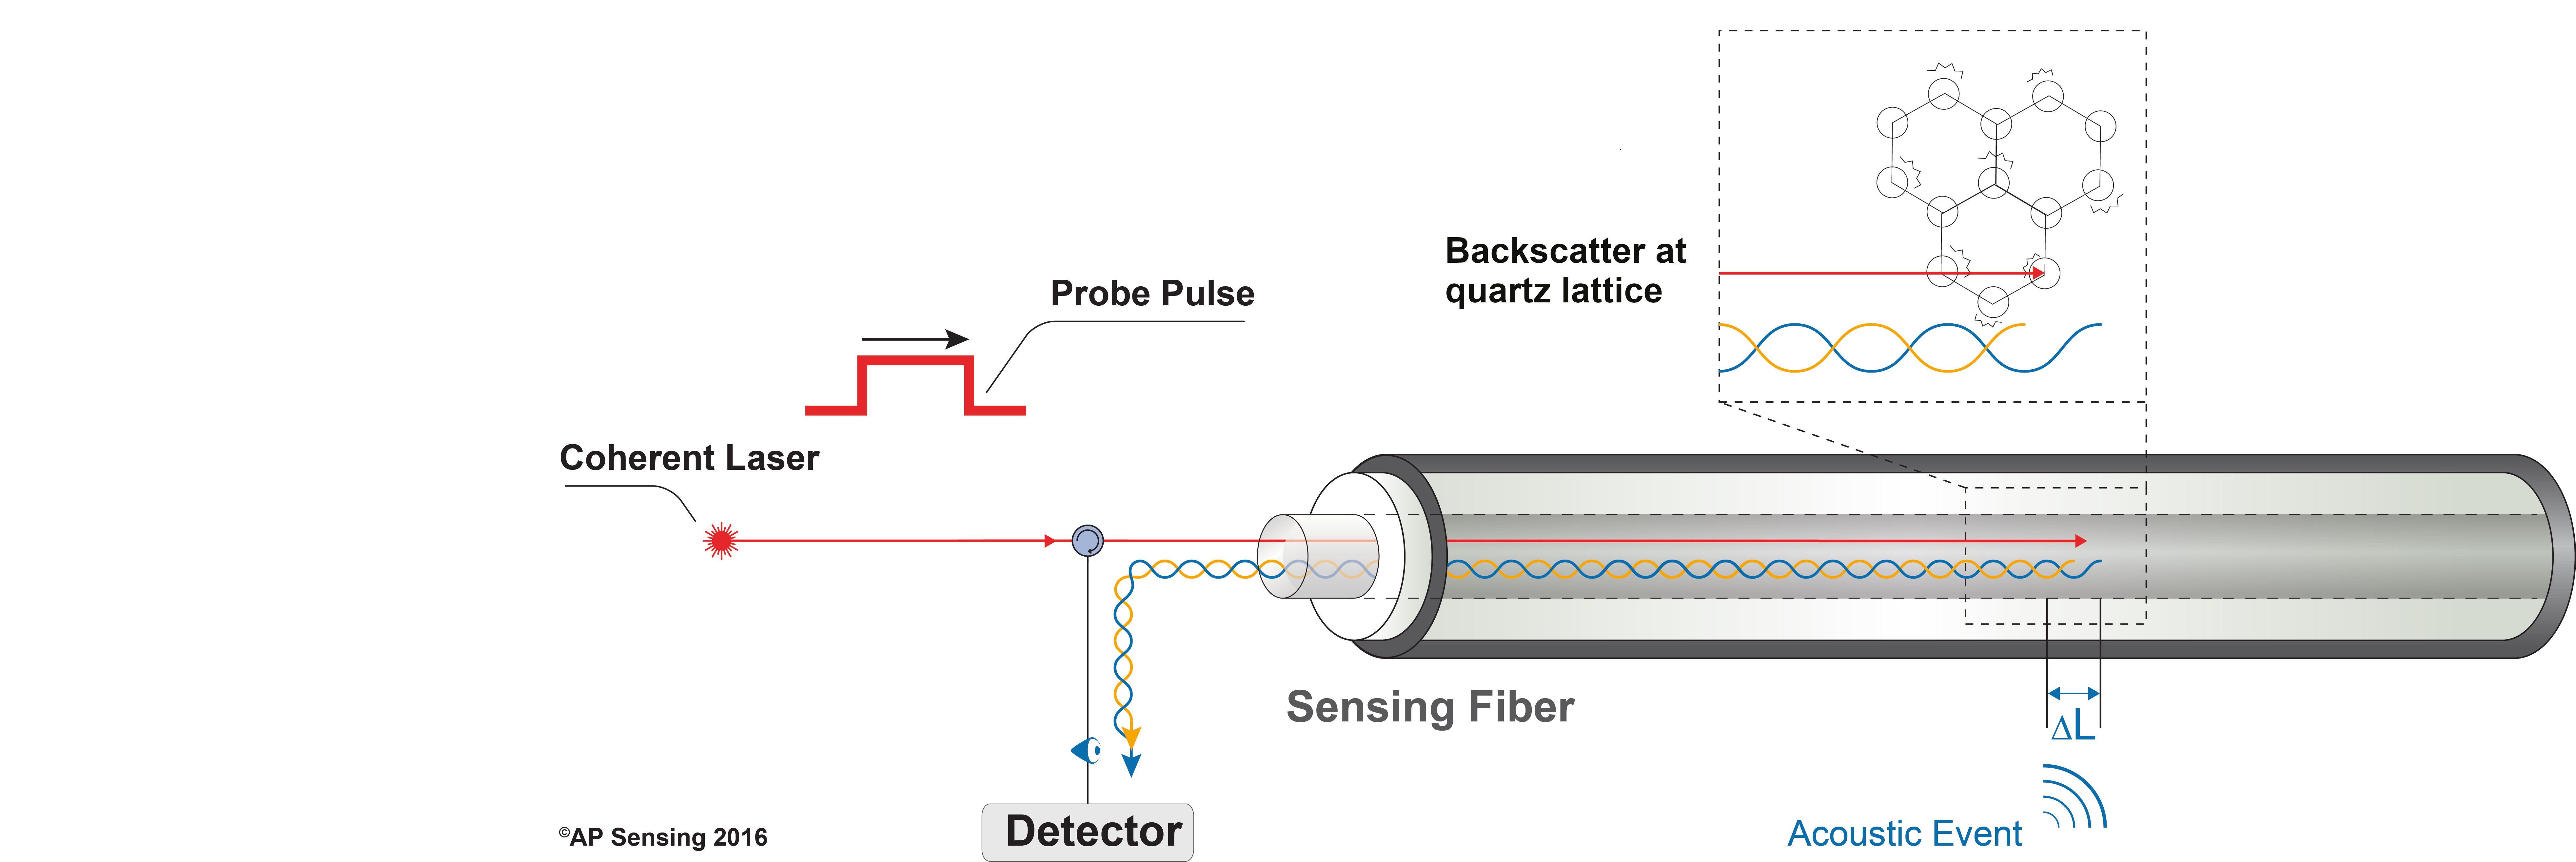
\includegraphics[width=0.7\linewidth]{Bilder/jpg/DAS_Acoustic_Event.jpg}
    \caption{Working principle of DAS system~\cite{DAS_Manual}}
    \label{DAS_working}
\end{figure}

Figure~\ref{DAS_working} shows how the laser is sent through the fiber optic cable and detected back after back scattering. When the acoustic event takes place, a tiny elongation or compression($\Delta L$) alters the phase relationship of the backscattered light signals. These signals are analyzed to show the frequency and amplitude disturbances. An Exact location of the acoustic event can be identified by measuring the time-dependent return of the light,  the same principle used in radar echos. 

\begin{figure}[h]
  \centering
  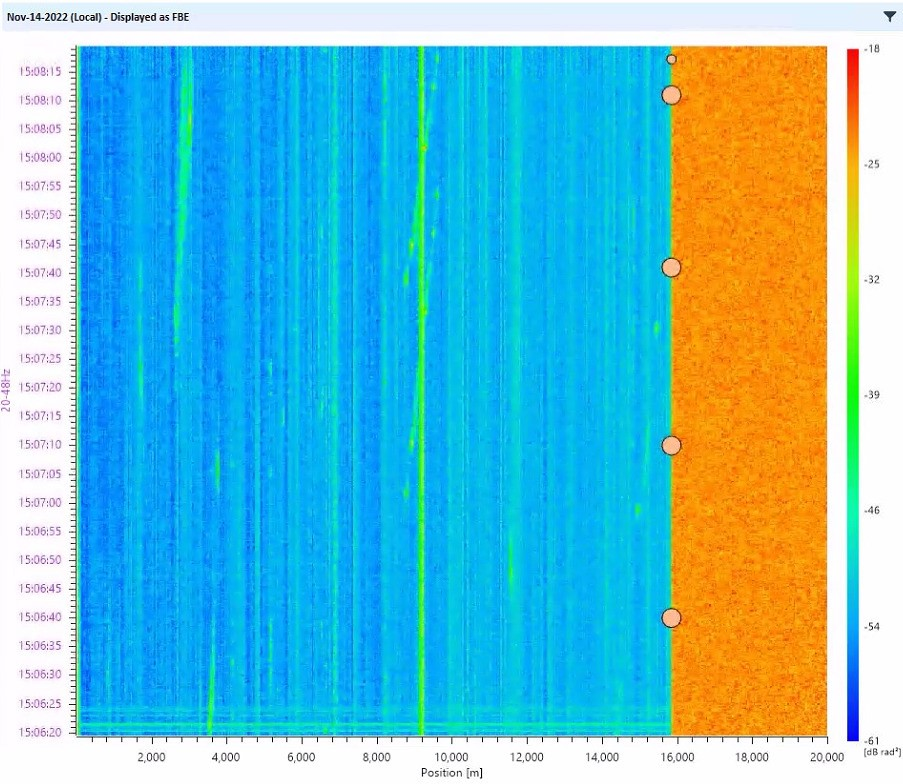
\includegraphics[width=0.7\linewidth]{Bilder/jpg/DAS Waterfall.jpg}
  \caption{Waterfall Diagram~\cite{Waterfall}}
  \label{DAS_waterfall}
\end{figure}

After digitizing and filtering the analog signals, the data can be processed and analyzed over distance and time and displayed in the form of a waterfall diagram as shown in the Figure~\ref{DAS_waterfall} where X-axis is the position on fiber and Y-axis is timestamp of recording. The data is recorded in the files in the HDF5 file format. The data from the HDF5 file is used to develop an algorithm which is used for the footsteps detection. Transforming the signal amplitude over time and in the frequency domain retrieves the acoustic event's frequency content. Using the acoustic event's location, amplitude, and frequency response, the system sets up an alarm for a potential threat-related activity. 

\subsection{AP Sensing DAS System}
There are two main components of the AP Sensing DAS system - the Interrogator Unit(IU) and the Digital Processing Unit(DPU). Figure~\ref{DAS} shows the IU(top) and DPU(bottom) which are the part of the DAS system.

\begin{figure}[h]
    \centering
    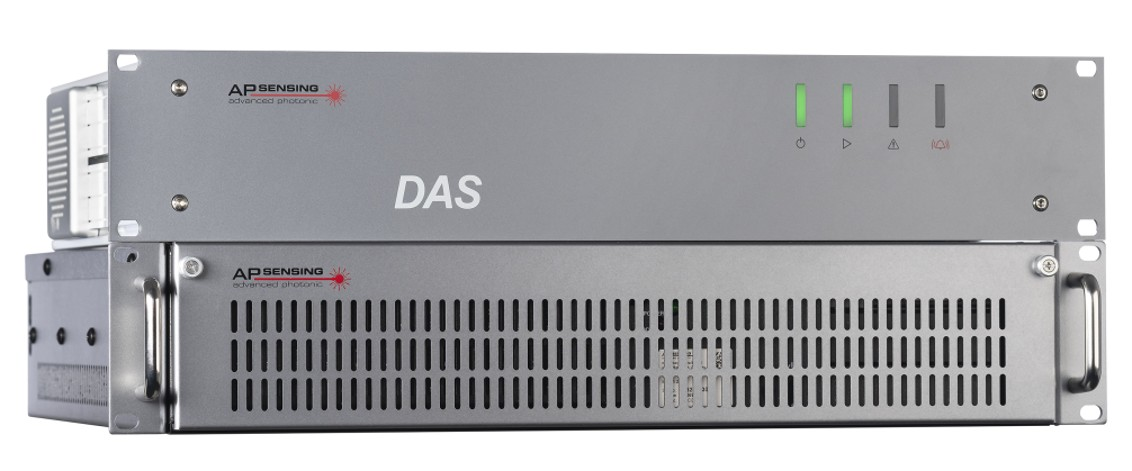
\includegraphics[width=\linewidth]{Bilder/jpg/DAS.jpg}
    \caption{AP Sensing DAS device~\cite{DAS_Manual}}
    \label{DAS}
\end{figure}

The IU(top) has the task of sending out highly coherent laser pulses into the fiber and thereby detecting the change in phase which is caused by Rayleigh backscattering. Analog signals containing the information in the form of frequency and amplitude are then sent to the DPU(bottom) for further processing. Figure~\ref{IU} shows the rear panel of the IU and all the ports present.

\begin{figure}[h]
    \centering
    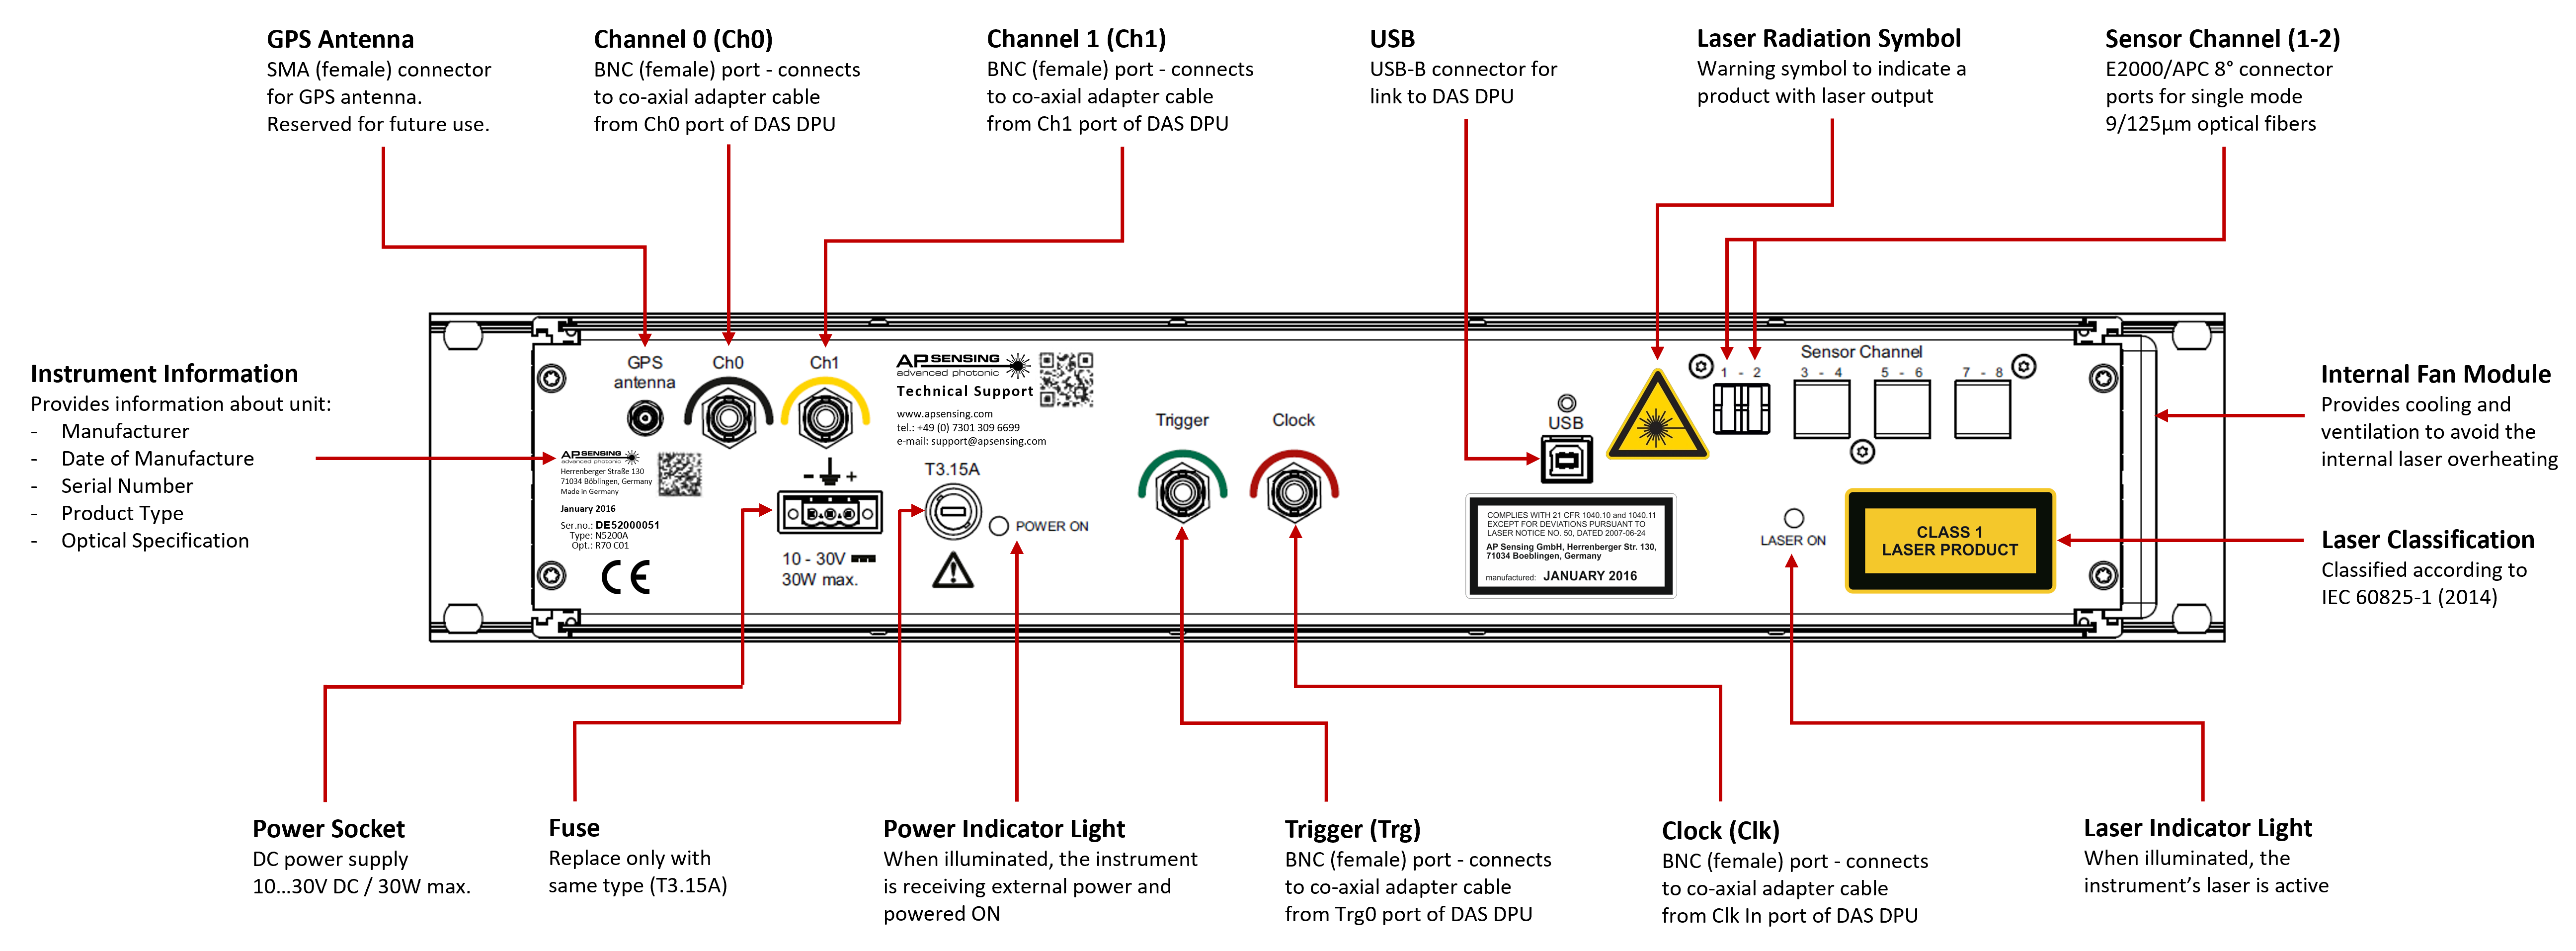
\includegraphics[width=\linewidth]{Bilder/jpg/DAS IU Technical Description.png}
    \caption{DAS IU rear panel view~\cite{DAS_Manual}}
    \label{IU}
\end{figure}

The IU(top) has two channels (horizontal and vertical polarization) which are connected to the DPU(bottom). A USB connector is also connected to the DPU(bottom). A Power socket is needed to power the IU. The trigger which is used to trigger sending of laser pulse is also connected to the DPU. A Digitizer inside the DPU(bottom) is used for synchronization between the IU(top) and DPU(bottom). The IU(top) contains a reference coil of 120m optical fiber inside the case unit. The primary function of this reference coil is to monitor system noise and to checkw whether equipment is measuring accurately. 

\begin{figure}[h]
    \centering
    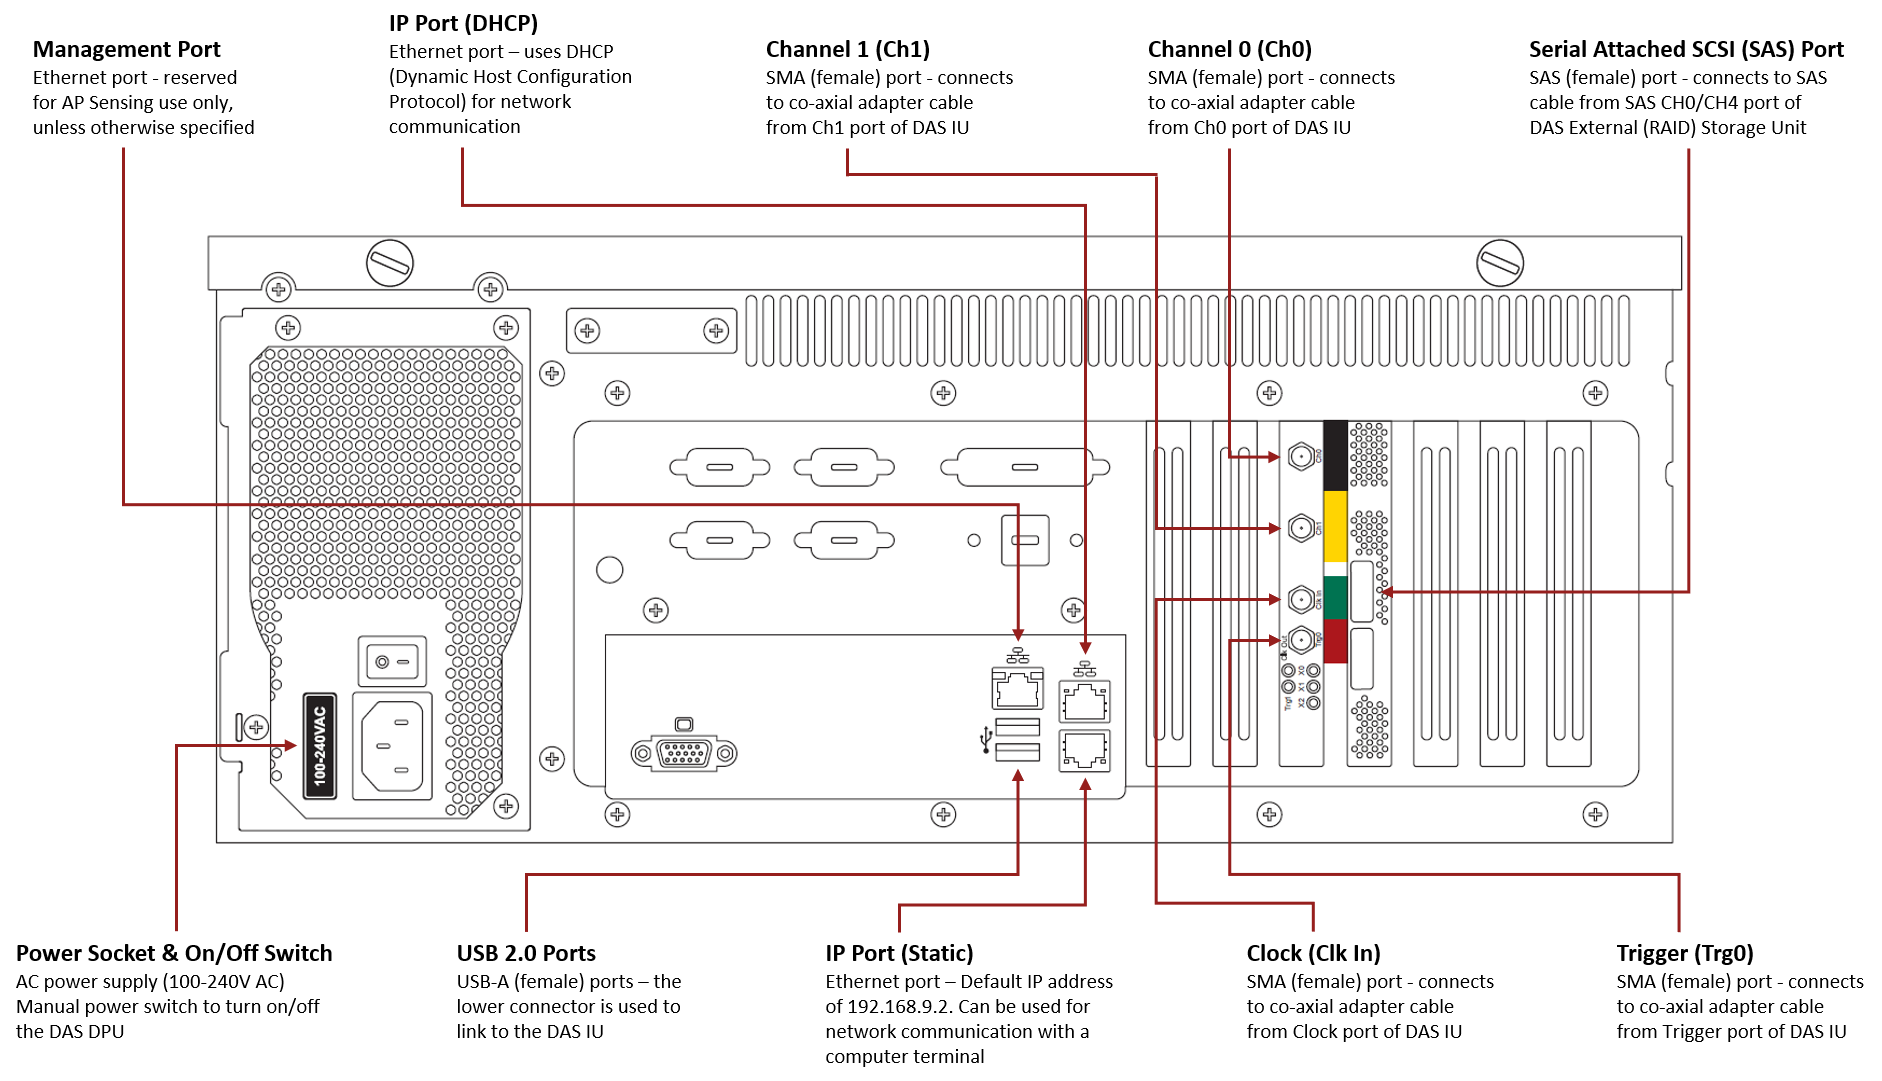
\includegraphics[width=\linewidth]{Bilder/jpg/DAS DPU Rear.png}
    \caption{DAS DPU rear panel view~\cite{DAS_Manual}}
    \label{DPU}
\end{figure}

Figure~\ref{DPU} show the rear view of the DPU of the DAS system. All the connections like the channels, USB, trigger and clock coming from the IU needs to be connected to the DPU. The DPU needs a separate power connection to power it up. There is also an Ethernet port which is used to connect the DAS system to network. The DAS system is connected to a computer via DAS Configurator application if the IP address of the system is known. All the calculations are started through this app. The data is stored in the form of HDF5 file. There are two SSDs available inside the DPU which can be used to store data. The stored data is automatically overwritten once when the capacity limit is reached, following the first-in, first-out (FIFO) approach. There is also other functionality that the data will be erased 30 days after the data is being stored. 

The data outputted from the DPU is made available in the three different formats. 

\begin{itemize} 
    \item{Phase (Dynamic Strain):} 
    This data type provides the raw signal of dynamic strain along the fiber, making it the most data-intensive of the three.

    \item{FBE (Frequency Band Energy):} 
    This data type aggregates the energy within each defined frequency band. After the backscattered signals are captured at each distance channel, they are divided into separate frequency ranges (e.g., 8-20 Hz). The total energy in each band is then displayed in the waterfall plot in Figure~\ref{DAS_waterfall} of the DAS Configurator Client. Its primary purpose is to differentiate between various acoustic events.

    \item{DTGS (Distributed Temperature Gradient Sensing):} 
    This data type highlights gradual variations in the signal arising from bulk temperature or strain effects. Conceptually, it functions like an additional low-frequency band, as the phase signal is analyzed at frequencies below 0.5 Hz.
\end{itemize}


\subsection{DAS Configurator Client}\label{sec:config_app}
DAS Configurator Application is an easy-to-use graphical interface for AP Sensing DAS systems. It allows users to configure and run measurements on the DAS system. The recording and saving of the measured data is also be done which can be useful for analysis and testing of trained models like ConvNext V2 and EfficientNet. It also helps in analyzing and visualization of the data. The data is collected from the DPU which acts as a server. It is designed to continuously run to record the data. The DAS client configurator application is installed on a separate computer which is connected to the DAS DPU via Ethernet. 

\begin{figure}[h]
    \centering
    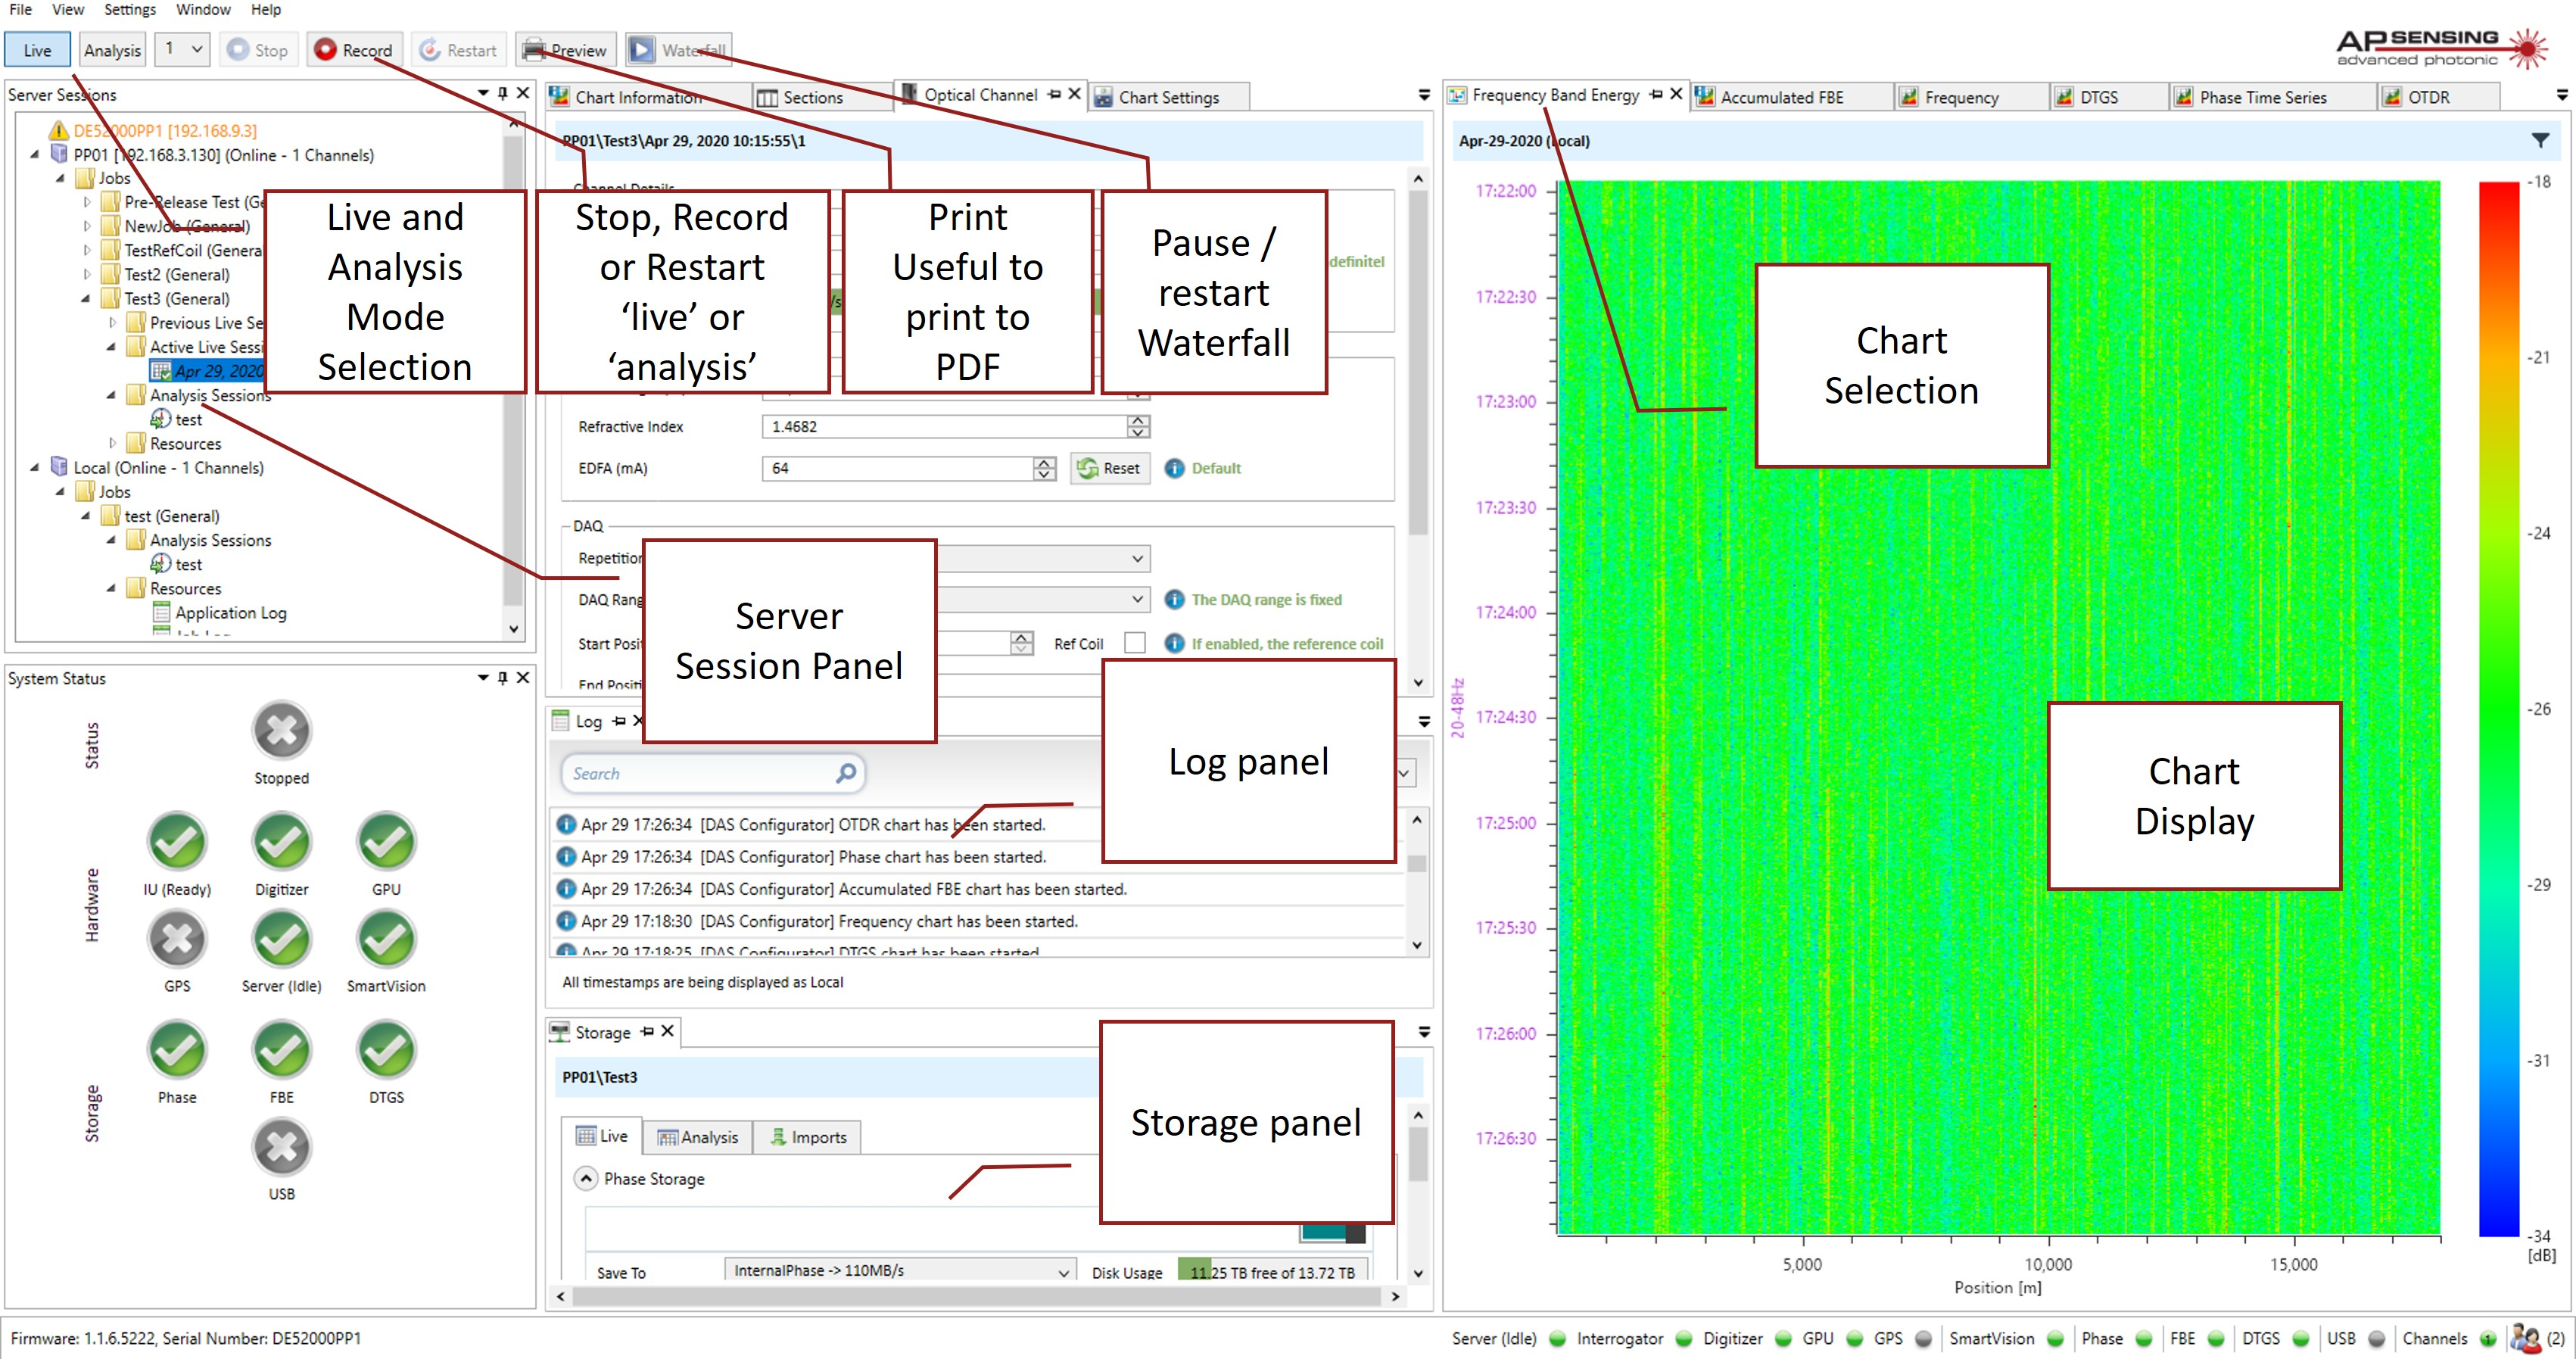
\includegraphics[width=\linewidth]{Bilder/jpg/DAS_config.jpg}
    \caption{Graphical Interface of DAS Configurator Application~\cite{DAS_Configurator_Manual}}
    \label{config}
\end{figure}

Figure~\ref{config} shows the graphical interface of the DAS Configurator Application. The top and bottom bars are fixed while all other charts and panels are easily configurable. They can be freely enabled or disabled. There is a live and analysis mode selection button which can be used to select the respective modes. Then the stop, record or restart button which can be used to the respective tasks with the session. The print button is used to print the screen to a pdf file. The pause/restart button is used to perform the respective operations on the waterfall diagram. Different charts like Phase, FBE and DTGS which can be selected for the layout. The server session panel where different recording session are stored in which all the data related to recording like the time of start and stop of the session, HDF5 files stored can be accessed. The storage panel  shows the available disk space on the drive. The log panel is used to keep the log of the events which happen during the entire session. 

\begin{figure}[h]
    \centering
    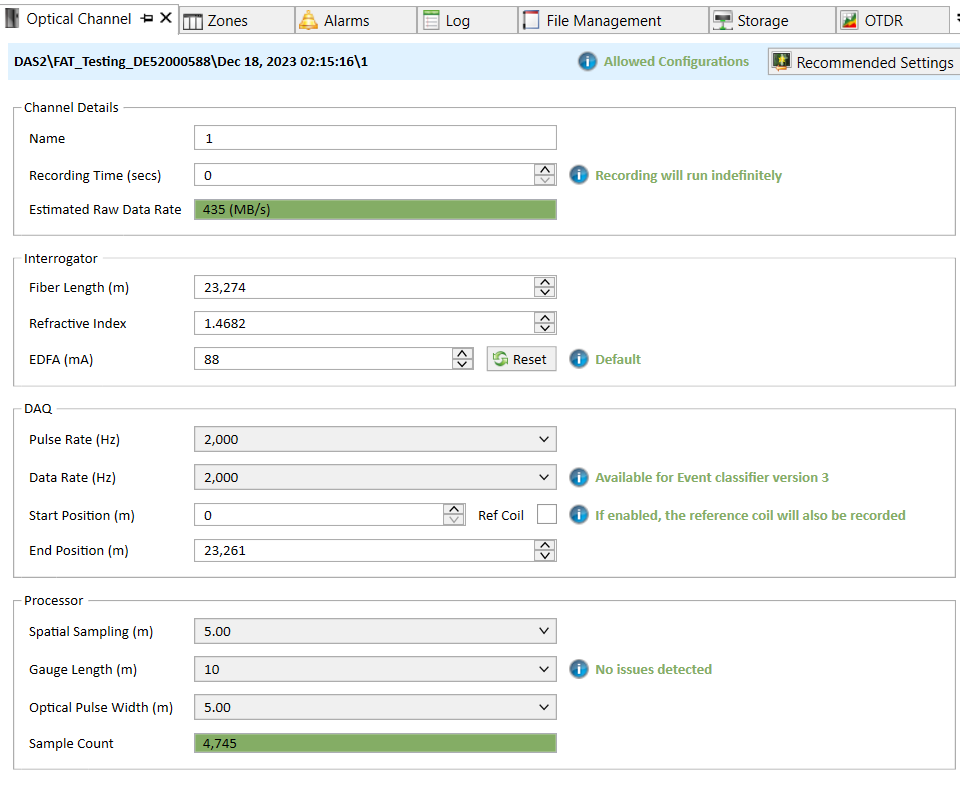
\includegraphics[width=0.8\linewidth]{Bilder/jpg/optical_channel.png}
    \caption{Optical Channel Window in DAS Configurator Application}
    \label{optical}
\end{figure}

Figure~\ref{optical} gives an overview of the optical channel settings that needs to be done on the DAS system. All the configuration settings for the session are done here. The system specifies the channel's name using the "name" field, and it defines the recording time as the duration (in seconds) for which the recording is performed. The maximum data is 960MB/s and if the date rate is exceeded the field turns orange and a warning message is displayed or else its green. Fiber length is actual length of the cable. Refractive index is 1.4682 which is the default value for the single mode fiber. The value can be changed if the manufacturers value of the fiber is different. EDFA value is to be kept unchanged and is adjusted by the production team at AP Sensing. Pulse rate is the laser pulse rate of the DAS interrogator and maximum rate can be given by (math equation). Data rate is the rate of output traces per second, which can be lower than Pulse Rate to allow oversampling. The start and end position are the positions of start and end point of the recording respectively. The spatial sampling is sampling rate along the fiber length and can be adjusted from 1.25m to 40m. Gauge length is the distance between two phase measurements, determining spatial resolution and can be in the range 3.75m to 80m. Optical pulse width is the actual physical width of the pulse, adjustable by trained user which affects the DAS performance. The sample count are the number of samples to be processed. These are the total points in the fiber that are responsible for collecting the data which then further used for plotting the waterfall diagram or stored in HDF5 format. User can select which data can select the format of data (Phase, FBE or DTGS) as explained in previous section. The data from HDF5 files can be retrieved using any programming language as there are already packages or libraries available which can be used to access them. 

\section{Image Recognition using Machine Learning}
Image Recognition is a process of detecting different patterns in the images and detecting similar images. Image Recognition is useful in crucial applications like autonomous vehicles, medical diagnosis and visual search. It has been revolutionized by deep learning techniques such as convolutional neural networks (CNNs) and recurrent neural networks (RNNs) as it has better performance for image recognition. Machine learning methods for image recognition rely on algorithms trained on extensive collection of images. These systems automatically detect patterns and visual elements(edges, textures and colors) critical for categorization. After the training phase where the model is trained on a particular set of images, the model can automatically detect similar sort of patterns and images thus enabling accurate and scalable image analysis~\cite{chandni}. 

For a model to detect the similar sort of patterns, it needs to be trained and evaluated on a dataset. The dataset needs to be collected where the different kind of images need to be labelled and based on these labels the model is trained. Different augmentation techniques are also applied to the training dataset such as flipping images or rotation. The model training is thus generalized and is able to detect the images correctly irrespective of what new images the model comes across. The model should be trained in such a way that it doesn't memorize the patterns in images but actually learns the patterns and generalize them properly. Evaluation of the model needs to be done on the entirely different dataset which is not used in training phase. The performance of the model is determined by how well it performs on the evaluation dataset.

\begin{itemize} 
    \item \textbf{Data Preparation:} 
    Preparing training and testing data by gathering the different kind of images on which the model needs to be trained. The preprocessing steps need to be applied on the images in Figure~\ref{sec:preprocessing}. These help in consistency of the data and help in proper visualization of the images.

    \item \textbf{Finding a model:} 
    The pre-trained models are the models which are trained on the image dataset available online. These models are trained on large datasets and are available for use. The models can be used as a starting point for the training. The model can be trained on the dataset available and then fine-tuned to get the best performance. The models can be used as a black box where the model is trained on the dataset and then used for evaluation. 

    \item \textbf{Train the Model:} 
    Training a model requires to provide a model with training data. Training data can be any form of images which are given to the model. Images are passed through various layers of the model from which understands the patterns. Model goes through this training data several times, the model will automatically determine the most crucial aspects. Model will acquire the ability to detect more characteristics and distinguish between various classes of data.

    \item \textbf{Evaluation Data:}
    To check whether the model is trained properly or not, the model needs to be evaluated on a different dataset which is not used in training phase. Evaluation dataset should be similar to the training dataset but should not contain any of the images from the training dataset. Evaluation dataset is used to check how well the model is trained and how well it can detect the patterns in the images. The performance of the model is determined using the confusion matrix. Confusion matrix is a table which shows the actual and predicted values of the model. Confusion matrix is used to check how well the model is trained and how well it can detect the patterns in the images. 
\end{itemize}

\subsection{PyTorch}\label{sec:PyTorch}
PyTorch~\cite{PyTorch_website} is a machine learning library that provides an imperative and Pythonic coding style, emphasizing ease of use, seamless debugging, and alignment with other scientific computing libraries, while maintaining efficiency and supporting hardware accelerators like GPUs. The trend started in domain specific languages such as APL, MATLAB, R which turned multidimensional arrays (also known as tensors) into objects supported by mathematical primitives to manipulate them. Other libraries such as NumPy, Torch, Eigen and Lush made array-based(tensor) programming productive in general purpose languages such as Python and C++~\cite{pytorch}. 

Deep learning is computations on tensors, which are generalizations of a matrix that can be indexed in more than 2D. Data required is extracted in the form of NumPy arrays. Arrays are preprocessed according to the requirement in such a way that patterns in the images are clearly visible. Then NumPy data is converted into a tensor which then feed to a model for training. The model trains based on this tensor. There are various metrics which need to be monitored while training the model to see if the model is learning efficiently and not memorizing the patterns. 

The efficacy of the model is the ability of a model to make the correct predictions. There are various metrics like Accuracy, Precision and Recall which need to be considered and are important to understand how well the model is trained. It revolves around categorizing the data points into predefined classes which is also known as classification problems. For instance, determining whether an email is a spam or not can be treated as an example of a binary classification. As the complexity of the model increases and the number of classes increase the intricacy of model increases. These metrics need to be monitored not only for the overall model but also over each class to see how well the model is classifying~\cite{Efficacy}. 

\subsubsection{Confusion Matrix}
The confusion matrix is a very important element in evaluating how well the model is trained. Model is improved by monitoring these metrics. The table~\ref{tab:confusion_matrix} shows the different metrics. The comparison of actual outcomes with predicted outcomes is done. The class imbalance is understood here and based on that it is determined whether the problem is with a specific class or the whole model. 

\begin{table}[ht]
    \centering
    \begin{tabular}{l|c|c|c}
      \toprule
      & \multicolumn{2}{c}{\textbf{Predicted}} & \\
      \cmidrule(lr){2-3}
      & \textbf{Positive} & \textbf{Negative} & \textbf{Total} \\
      \midrule
      \textbf{Actual} \tabularnewline
      \textbf{Positive} & True Positive (TP) & False Negative (FN) & Total Positive \\
      \midrule
      \textbf{Negative} & False Positive (FP) & True Negative (TN) & Total Negative \\
      \midrule
      \textbf{Total} & Total Predicted Positive & Total Predicted Negative & Total Samples \\
      \bottomrule
    \end{tabular}
    \caption{Confusion Matrix Example}
    \label{tab:confusion_matrix}
  \end{table}

  The four main elements can be explained as follows which will give an overview of the models expected and actual outputs.
  \begin{itemize}
    \item \textbf{True Positive (TP)}:  The model correctly identifies instances belonging to the positive class. \\
      \textit{Example}: Spam emails automatically routed to the spam folder.

      \item \textbf{True Negative (TN)}: The model accurately identifies instances belonging to the negative class \\
      \textit{Example}: Important emails delivered directly to the inbox.
  
        \item \textbf{False Positive (FP)}: The model incorrectly classifies negative instances as positive (Type I error).
      \textit{Example}: Important emails mistakenly sent to the spam folder.
  
    \item \textbf{False Negative (FN)}:The model fails to identify positive instances, classifying them as negative (Type II error). \\
      \textit{Example}: Spam emails slipping through the filter and appearing in the inbox.
  
  \end{itemize}

  There are different metrics like accuracy, precision and recall which can be calculated using the elements from the table~\ref{tab:confusion_matrix}. Ideally all the values should be high but depending on the use case the values are traded off to give the best performance for the case. Accuracy can be misleading as it fails to measure overall correctness when classes are imbalanced. So precision or recall need to be used to identify the performance of the minority class. The spam email detection example will give the better understanding for the same. The model labels all email not spam would get 95\% accuracy but fails to detect any spam. If the model detects 80\% of spam emails(high recall) but mislabels 20\% of the legitimate emails(low precision) user can get annoyed by false alarms. 

  \subsubsection{Accuracy}
  Accuracy is a metric that quantifies the overall performance of a classification model by measuring the proportion of correctly predicted instances (both true positives and true negatives) relative to the total number of instances. It is calculated using the formula:

  \begin{equation}
    \text{Accuracy} = \frac{TP + TN}{TP + TN + FP + FN} \times 100\%
    \label{eq:accuracy}
  \end{equation}
  where:
  \begin{itemize}
    \item $TP$ = True Positives
    \item $TN$ = True Negatives
    \item $FP$ = False Positives
    \item $FN$ = False Negatives
  \end{itemize}

  Accuracy is often the first metric evaluated for classification tasks due to its simplicity and intuitive interpretation as a percentage of correct predictions. It works well when the dataset has balanced class distributions. However in imbalanced scenarios other metrics also need to be considered. In real life scenarios the cost of false negative (failing to identify a disease) might be more severe than a false positive in a medical diagnosis.

  \subsubsection{Precision}
  Precision is a metric providing how well the model predicts positive instances while minimizing the risk of false alarms. Precision is an important metric in classification problems where the cost is high for false positives. Precision is true positives from all positives detected by the model. The precision of a classification model is calculated as:

  \begin{equation}
    \text{Precision} = \frac{TP}{TP + FP} \times 100\%
    \label{eq:precision}
  \end{equation}
  where:
  \begin{itemize}
    \item $TP$ = True Positives
    \item $FP$ = False Positives
  \end{itemize}

  Precision is very important when false positives are costly. False positives are very costly in instances like fraud detection systems, where flagging legitimate transactions leads to unnecessary investigation and customer dissatisfaction, potentially causing business loss. Precision only focuses on positive cases, neglecting all negative cases. A model achieves high precision by making fewer positive predictions, resulting in missing many positive cases.

\subsubsection{Recall}
Recall is a metric representing the proportion of actual positive cases identified by the model. Recall is also known as sensitivity or the true positive rate. The recall of a classification model is calculated as:

\begin{equation}
  \text{Recall} = \frac{TP}{TP + FN} \times 100\%
  \label{eq:recall}
\end{equation}
where:
\begin{itemize}
  \item $TP$ = True Positives
  \item $FN$ = False Negatives
\end{itemize}

Recall is important where false negatives are costly. Recall focuses on finding all positive cases even with more false positives. A model may predict most instances as positive to achieve high recall. This leads to many incorrect positive predictions. Using these metrics and making adjustments as needed, the model is trained according to requirements. 

\subsection{Data Augmentations}\label{sec:augmentation}
Data augmentation implies a collection of different techniques  to enhance the diversity and volume of training datasets to improve the model performance. The techniques include geometric transformations, color space adjustments, filter-based adjustments, filter-based methods, image mixing, random erasing. This helps in improving model generalization and diversifying the dataset thus helping in dealing with overfitting problem~\cite{Augmentation}. 

The data augmentation helps in generalizing the data better which will help in training the model with the patterns instead of model memorizing the images. Model will perform better on the unseen data when augmentation techniques are used. 

\subsubsection{Horizontal Flipping}
Horizontal flipping mirrors the image along the vertical axis, thus creating a horizontally reversed image. This helps model to generalize better thus reducing the overfitting. Figure~\ref{hflip} shows the horizontal flip of cat image.

\begin{figure}[h]
    \centering
    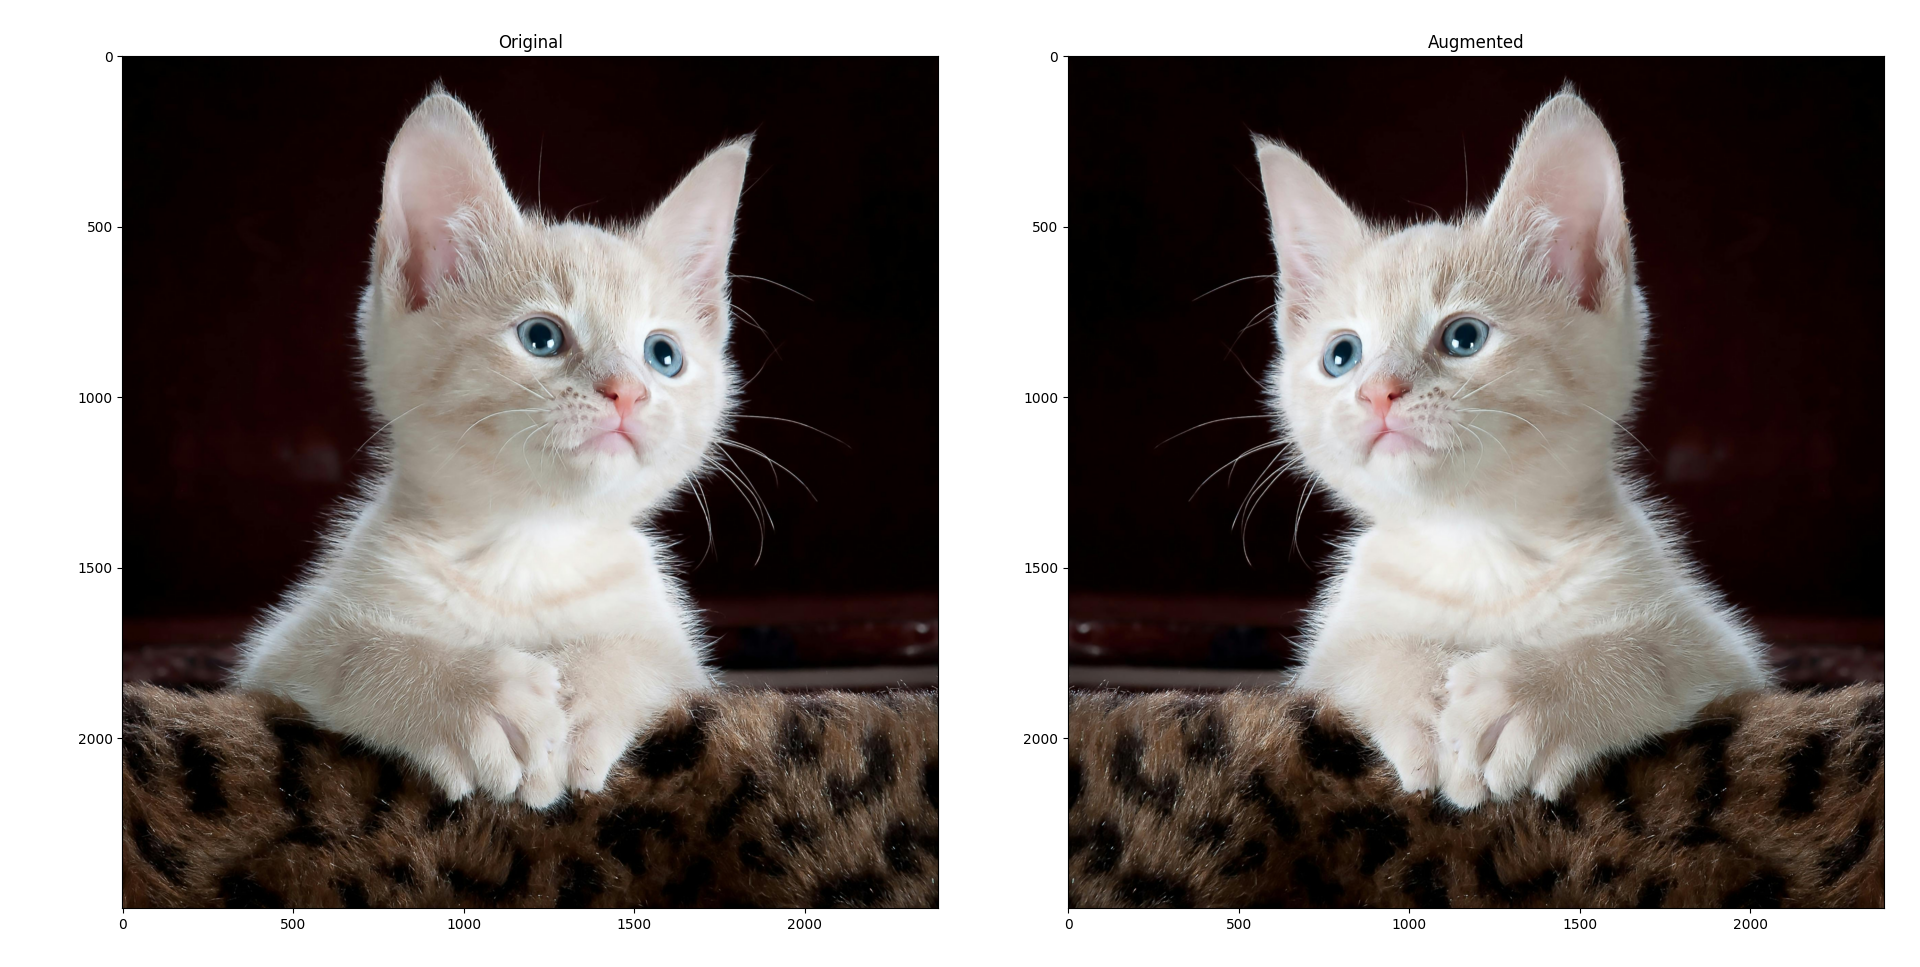
\includegraphics[width=0.6\linewidth]{Bilder/jpg/Horizontal flip.png}
    \caption{Horizontal Flip~\cite{kitten}}
    \label{hflip}
\end{figure}

\subsubsection{Vertical Scaling}
Vertical scaling or amplitude scales the image on the vertical or amplitude scale, thus creating image which is stretched along the vertical or amplitude axis. This also helps in generalization and detects images which are stretched on the vertical scale. Figure~\ref{amp} shows it with cat image how the image is stretched along the vertical scale or amplitude scale .

\begin{figure}[h]
    \centering
    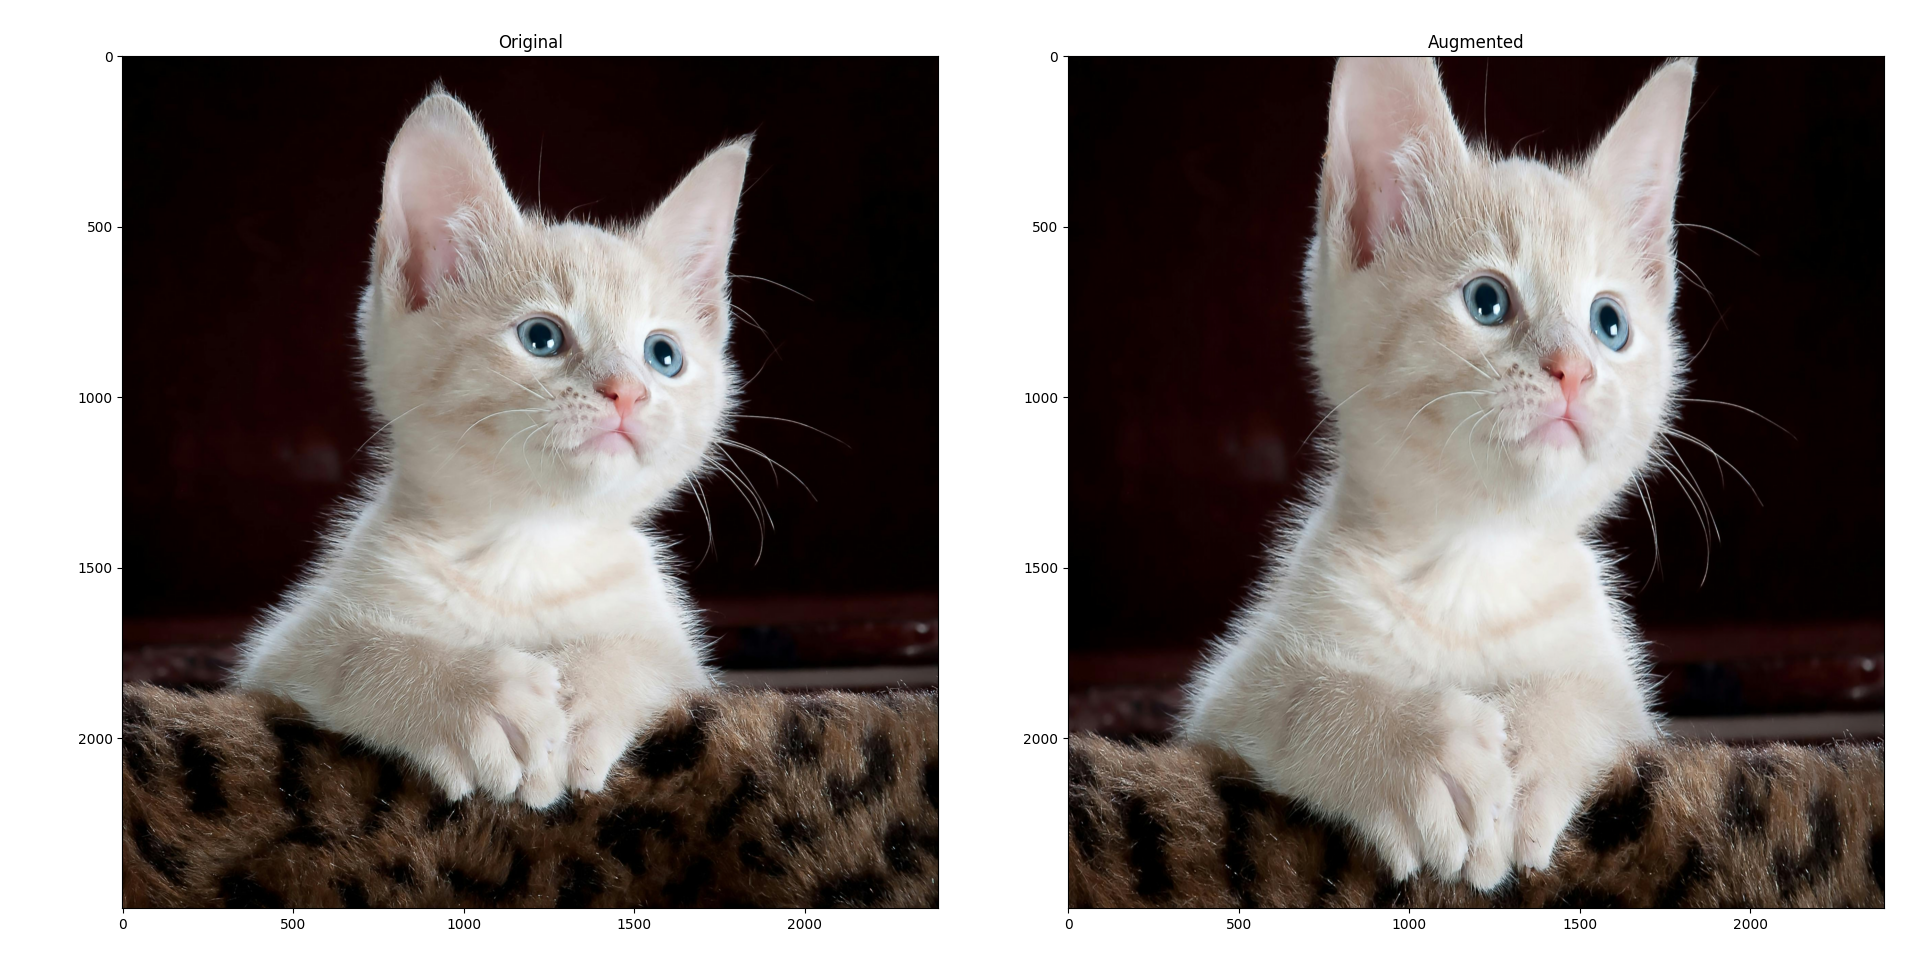
\includegraphics[width=0.6\linewidth]{Bilder/jpg/amp.png}
    \caption{Vertical Scaling~\cite{kitten}}
    \label{amp}
\end{figure}

\subsubsection{Horizontal Scaling}
Horizontal scaling or time scaling is amplifying the image across the time scale or horizontal scale , thus creating image which is stretched across the time or horizontal axis. This also helps in generalization and even if the images which are stretched on horizontal scale. Figure~\ref{time} shows this with a cat image where it is stretched along the time scale or horizontal scale for. 

\begin{figure}[h]
    \centering
    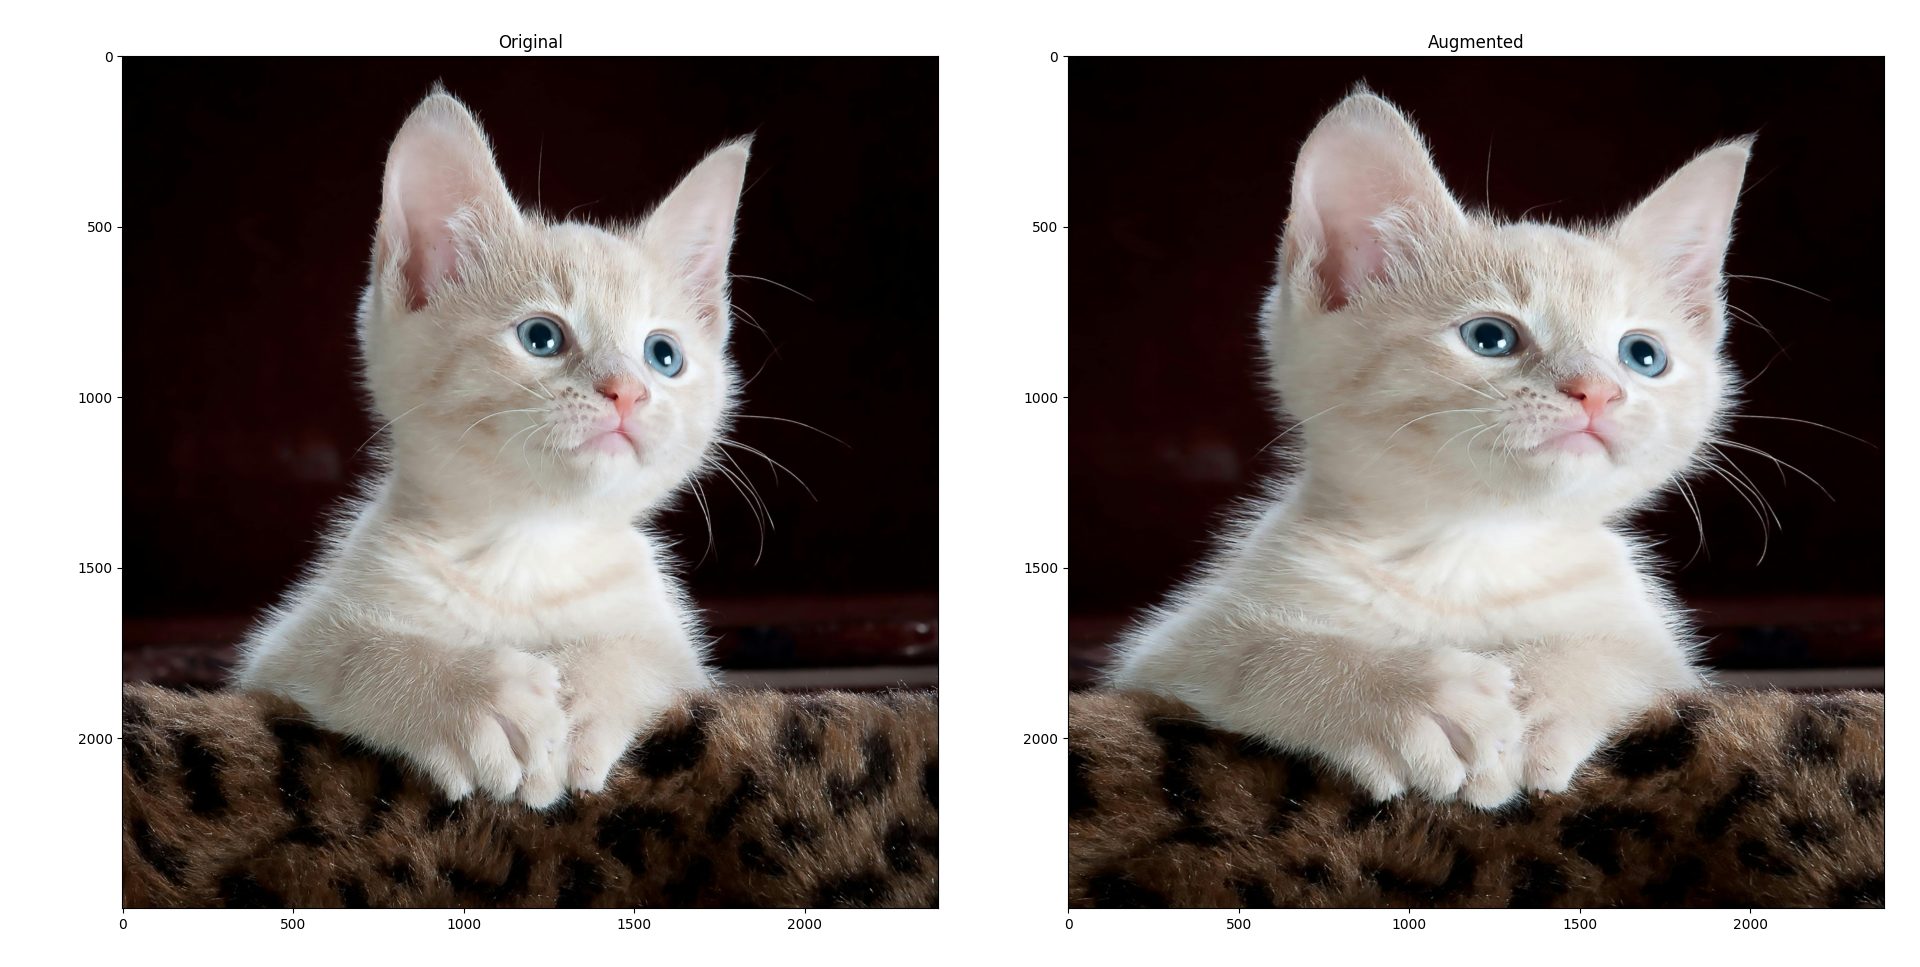
\includegraphics[width=0.6\linewidth]{Bilder/jpg/affine.png}
    \caption{Horizontal Scaling~\cite{kitten}}
    \label{time}
\end{figure}

\subsubsection{Gaussian Noise Injection}
In this augmentation, gaussian noise is injected into the image to increase the robustness and generalization of the model. The noise is added to the image by controlling the mean and standard deviation. Figure~\ref{noise} demonstrates injecting the noise to a cat image with standard deviation set to 0.6 for demonstration purposes so that injection is visible.

\begin{figure}[h]
  \centering
  \includegraphics[width=0.6\linewidth]{Bilder/jpg/Noise.png}
  \caption{Gaussian Noise Injection~\cite{kitten}}
  \label{noise}
\end{figure}

\subsection{Kornia}

Kornia is an open-source computer vision library built on top of PyTorch\ref{sec:PyTorch} that provides a familiar, NumPy-like API for classical vision operations (e.g.\ geometric transforms, filtering, feature detection) in a fully differentiable and GPU-accelerated form. Unlike the traditional 'torchvision.transforms'~\cite{torchvision2024}, which execute many augmentations on the CPU and then copy results to the GPU, Kornia implements each operation as a native PyTorch module or function that runs directly on CUDA. This tight integration allows to include data augmentations as part of the model's computation graph-making them differentiable, reducing host-device synchronization overhead, and enabling end-to-end optimization when desired.

In our spectrogram-based footstep classification pipeline, we use several Kornia augmentations (Horizontal Flip, Normalize) alongside custom PyTorch modules.  By leveraging Kornia, we gain:

\begin{itemize}
  \item \textbf{Performance}: All transformations (flips, normalizations, warps) execute directly on the GPU, avoiding costly host-device transfers (i.e., data is not sent back to the CPU for processing) and achieving higher throughput during training.
  \item \textbf{Differentiability}: Since each augmentation is a PyTorch module, gradients can flow through the transform when performing adversarial or meta-learning experiments that require backpropagation through data augmentation.
  \item \textbf{Composability}: Kornia's ops follow the same 'torch.nn.Module' and functional API conventions as PyTorch, allowing seamless integration into 'torchvision.transforms.Compose', 'torch.nn.Sequential', or custom training loops.
\end{itemize}

Together, these features make Kornia an ideal choice for high-performance, flexible data augmentation in end-to-end deep-learning pipelines~\cite{kornia}. 

\section{Literature Review}
DAS has emerged as a versatile tool in detection of various human activities, including footsteps by sensing the ground vibrations. Over the past decade, researchers have explored signal processing, Machine learning (ML), and environmental adaptions to enhance the detection accuracy. This section gives an overview of different studies which shows key advancements and challenges.

\paragraph{Time-frequency preprocessing.}
A crucial first step is turning raw DAS phase traces into a time-frequency representation that makes footsteps stand out. Ekimov and Sabatier~\cite{ekimov2007ultrasonic} showed that human footsteps produce strong components in the 1-4~Hz band (with measurable energy up to 600~Hz outdoors) and used short-time Fourier transforms (STFTs) and spectrograms to isolate these bands. Likewise, K \textit{et al.}~\cite{ks2021acoustic} created synthetic datasets by slicing DAS recordings into 2~s windows and converting them into spectrograms-an approach we adopt directly, since it balances temporal resolution with computational cost.

\paragraph{Deep-learning classification.}
Once a spectrogram is in hand, convolutional neural networks (CNNs) have become the workhorse. Jakkampudi \textit{et al.}~\cite{footstep} applied a CNN to 5~km of outdoor DAS data (2~m channel spacing) and reported 84\% footstep vs background accuracy. To handle overlapping footsteps and changing directions, hybrid ConvLSTM architectures~\cite{zhou2024large} have been proposed improving indoor tracking accuracy to about 81.5\%. In our thesis, we build on these successes by comparing two state of the art backbones (ConvNeXt V2 and EfficientNet) and by introducing a targeted augmentation strategy to further reduce false negatives in challenging overlap scenarios.

\paragraph{Environment and noise adaptation.}
Outdoor DAS must contend with wind and distant traffic noise, while indoor signals suffer multipath reflections. Ekimov~\cite{ekimov2007ultrasonic} emphasized that vibration energy above 600~Hz decays rapidly outdoors, which motivates our choice of filter bank design. Bublin~\cite{bublin2021event} showed that combining DAS with auxiliary sensors (e.g.\ accelerometers) can improve robustness to transient events like excavator digging. Although we focus on single-sensor DAS here, our evaluation framework logs false-positive cases for future data-driven noise modeling or multimodal fusion.

\paragraph{Open challenges.}
Most prior work handles a single pedestrian or controlled corridor; detecting multiple simultaneous footsteps remains hard~\cite{footstep}. We likewise observe increasing false positives when multiple subjects share the same fiber segment. To address this, our model training pipeline incorporates random spatial and amplitude perturbations (Section~\ref{sec:augmentation}) to encourage separation of overlapping patterns laying groundwork for multi-person DAS detection in future extensions.

\paragraph{Benchmarking ML on DAS.}
Shi and Zong~\cite{Shi2025Benchmark} present one of the first end-to-end benchmarks comparing classical ML methods (SVM, Random Forest) against modern deep nets (CNNs, Transformers) on real DAS footstep data. They systematically evaluate different spectrogram parameters, data-augmentation recipes, and backbone architectures, and find that a lightweight vision-transformer slightly outperforms CNNs once trained with sufficient augmentation. Their results both validate our choice of ConvNeXt V2 and EfficientNet and underscore the importance of tuning augmentation hyperparameters.

\paragraph{Multimodal contrastive learning.}
Yadav \textit{et al.}~\cite{Yadav2021Contrastive} fuse DAS spectrograms with co-recorded geophone signals in a metric-learning framework. By pulling together matching footstep pairs across sensors and pushing apart non-footstep pairs, they learn a joint embedding that boosts classification accuracy by 15-20 pp over single-sensor baselines. Although our current work is purely DAS-based, their fusion approach offers a clear path to tackle the false-positive challenges we observe when multiple subjects overlap (Section~\ref{sec:augmentation}).

\medskip
By combining the spectrogram windowing strategy of~\cite{ks2021acoustic}, the CNN-based classifiers of~\cite{footstep} and~\cite{zhou2024large}, the rigorous benchmarking from~\cite{Shi2025Benchmark}, and the multimodal fusion ideas of~\cite{Yadav2021Contrastive}, this thesis delivers a robust, end-to-end footstep detector on both single- and ten-channel DAS data.

%
% Kapitel2.tex
%
\chapter{System Design}
\label{sec:system_design}
In this chapter, the end-to-end system design for capturing, processing, and leveraging phase data for training deep learning model training is presented. The experimental setup used describes the DAS deployment at the Energy Center in Hulb(B\"oblingen), the fiber-optic cable layout, and the HDF5 format~\cite{hdf5} used to archive raw phase measurements. Introduction to a modular data processing pipeline from ingestion and HDF5 file handling, through STFT-based spectrogram generation and logarithmic scaling, to final data serialization illustrated via a block diagram that highlights each stage inputs, outputs, and dependencies. Finally, the model training and testing framework, specifying how ConvNext V2 and EfficientNet will consume these preprocessed spectrograms is outlined.

\section{Experimental Setup for data acquisition}\label{sec:experimental_setup}
Data acquisition represents a fundamental component of this work, and every effort has been made to ensure that the collection process is robust and methodologically sound. The data is gathered using the DAS configurator application, as discussed and elaborated upon in section~\ref{sec:config_app}, it is then downloaded in HDF5 format. The data source is the Energy Building near the AP Sensing main office, where the DAS (Distributed Acoustic Sensing) system is installed. The DAS system, which operates using a state-of-the-art fiber optic cable deployed along a well-defined spatial route, captures walking patterns and other relevant phenomena. Figure~\ref{energiezentrale} illustrates the complete fiber optic cable layout deployed at the Energy Building. This visualization is essential, as it provides context for the subsequent analysis and aids in understanding the spatial distribution of the data.

\begin{figure}[ht]
    \centering
    \includegraphics[width=\linewidth]{Bilder/jpg/energiezentrale.png}
    \caption{Fiber optic layout at the Energy Center \cite{energy_ppt}}
    \label{energiezentrale}
\end{figure}

The fiber-optic cable begins at the AP Sensing office (yellow) and then traverses four segments before reaching Herrenberger Street:

\begin{itemize}
    \item \textbf{Trench near the fence (red, underground):}  
          The cable runs below ground alongside the perimeter fence.
    \item \textbf{Fence line (green, above ground):}  
          The cable is mounted directly onto the fence structure.
    \item \textbf{Distant trench (blue, underground):}  
          The cable returns underground in a trench set back from the fence.
    \item \textbf{Final approach (purple, underground):}  
          The cable continues beneath the ground toward Herrenberger Street.
\end{itemize}

Four numbered junctions mark critical splice and access points (Figure~\ref{energiezentrale}):

\begin{itemize}
    \item \textbf{Junction 1:} Splice box receiving input from the AP Sensing office and feeding out to the building perimeter.
    \item \textbf{Junction 2:} Splice box receiving the perimeter feed and directing it onward toward Herrenberger Street.
    \item \textbf{Junction 3:} Main manhole outside the fence for underground routing.
    \item \textbf{Junction 4:} Smaller pit adjacent to the fence, also used for underground transitions.
\end{itemize}

This layout enables precise spatial localization of acoustic events along the cable route. The footstep data is recorded from the setup by walking around the cable route and logging it properly. DAS system records phase data that reflects variations corresponding to walking patterns. Phase data is stored in an in the HDF5 file in the form of \texttt{xarray} format a multi-dimensional data structure well-suited for handling large, complex datasets. Attributes such as data rate, gauge length, spatial channels  which are set at the time of recording are stored in the HDF5 file in the form of metadata. 

\section{General structure of the system}
\begin{figure}[ht]
    \centering
    % Scale to fit page width
    \resizebox{\textwidth}{!}{%
      \begin{tikzpicture}[
        node distance=0.4cm and 0.6cm,
        >=Stealth,
        block/.style={
          rectangle,
          draw,
          rounded corners,
          text centered,
          minimum width=1.4cm,
          minimum height=0.9cm,
          font=\small,
          fill=gray!10
        }
      ]
      % Define nodes in a single row
      \node[block] (acq) {DAS Acquisition};
      \node[block, right=of acq] (extract) {Extraction};
      \node[block, right=of extract] (preproc) {Preprocessing};
      \node[block, right=of preproc] (dataset) {Dataset Creation};
      \node[block, right=of dataset] (train) {Training};
  
      % Draw arrows
      \draw[->] (acq) -- (extract);
      \draw[->] (extract) -- (preproc);
      \draw[->] (preproc) -- (dataset);
      \draw[->] (dataset) -- (train);
      \draw[->, dotted] (train.north) -- ++(0,1) -| (acq.north);
    \end{tikzpicture}%
    }
    \caption{Block diagram of the general structure of the system}
    \label{fig:footstep-pipeline}
  \end{figure}
  
  Figure~\ref{fig:footstep-pipeline} illustrates the general structure of the system what the thesis is trying to achieve. The system captures the data using the DAS system from the Energy building as explained in section~\ref{sec:experimental_setup}. The walking data is recorded by taking into the consideration the layout of the cable and logging needs to be done properly to determine the exact time and spatial location along the cable where the footsteps are recorded. 

  The data is stored in the HDF5 format which stores the phase data with timestamps and the spatial locations. The footstep data is extracted from the HDF5 file and needs to be stored separately which is needed for training the model. Also, different types of background noise needs to be extracted from the HDF5 file which is needs for the model training. For clear distinction between the footsteps ans background data the data is preprocessed (section~\ref{sec:preprocessing}) and converted into spectrograms. The spectrograms are then used to create the dataset which is used for training the model. The spectrograms are used as the clear distinction between footsteps and background noise can be seen in the spectrograms. Using these spectrograms the model is trained and evaluation is done based on the accuracy of the model. 
  
\section{Internal Structure}
Internally the structure of the system is split into various blocks as shown in Figure~\ref{fig:footstep-pipeline}. The blocks are explained in detail in the following sections. The blocks are designed in such a way that they can be used independently and can be reused for other applications as well. Each block from Figure~\ref{fig:footstep-pipeline} has further smaller blocks which are explained in the following sections. 

\subsection{Data Acquisition}\label{sec:data_acquisition}
In the section~\ref{sec:experimental_setup} it is explained how the fiber optic cable is laid and using the DAS configurator application the data is recorded. The data is stored in the HDF5 format which is a file format used to store large amounts of data. Figure~\ref{fig:daq-simple} gives the overview of data acquisition process. The data acquisition block is the main block from Figure~\ref{fig:footstep-pipeline} which records the data from the DAS setup using the DAS configurator application and stores it in the HDF5 file format. The phase data from this HDF5 file further visualized using the RGB array.

\begin{figure}[ht]
  \centering
  \resizebox{\textwidth}{!}{%%
    \begin{tikzpicture}[
      node distance=1cm,
      >=Stealth,
      subblock/.style={
        rectangle,
        draw,
        rounded corners,
        text centered,
        minimum width=2.5cm,
        minimum height=0.8cm,
        font=\scriptsize,
        fill=blue!10,
      },
      container/.style={
        rectangle,
        draw,
        thick,
        rounded corners,
        fill=gray!20,
      }
    ]
    % Layers
    \pgfdeclarelayer{background}
    \pgfsetlayers{background,main}

    % Sub-blocks
    \node[subblock] (rec) {Recording};
    \node[subblock, right=of rec] (hdf) {HDF5 Storage};
    \node[subblock, right=of hdf] (viz) {Visualization};

    % Draw arrows
    \draw[->] (rec) -- (hdf);
    \draw[->] (hdf) -- (viz);

    % Container in background
    \begin{pgfonlayer}{background}
      \node[container, fit=(rec) (hdf) (viz), inner sep=10pt] (daq) {};
      \node[anchor=north west, font=\scriptsize] at (daq.north west) {Data Acquisition};
    \end{pgfonlayer}
  \end{tikzpicture}%%
  }
  \caption{Data acquisition block: Recording phase data, storing in HDF5 format, and visualizing the data.}
  \label{fig:daq-simple}
\end{figure}
The data in HDF5 file is stored in the form of xarray format. The xarray format is a multi-dimensional data structure that allows for easy manipulation and analysis of large datasets. The phase data is stored in the HDF5 file with timestamps and the distance along the cable route at which the data is recorded. For better viewing the data is converted into a DataFrame which is a tabular format~\cite{mckinney2010data}. DataFrame contains the phase data with timestamps and the distance along the cable route at which the data is recorded. Table~\ref{tab:phase_data} shows the phase data in the form of a matrix with the distance along the cable route on the x-axis and time on the y-axis. Each cell in the table represents the phase data at a specific distance and time. 

\begin{table}[ht]
  \centering
  \resizebox{\textwidth}{!}{%
    \begin{tabular}{l r c r c r}
      \toprule
      & \multicolumn{5}{c}{\textbf{Distance (m)}} \\
      \cmidrule(lr){2-6}
      \textbf{Timestamps (UTC)} 
        & 53638.285156 & \dots & 53701.992188 & \dots & 53726.496094 \\
      \midrule
      2024-10-21 10:27:40.000183+00:00 
        &   243.9019   & \dots & 1105.7420    & \dots &   854.9858    \\
      2024-10-21 10:27:40.001183+00:00
        &  -908.2096   & \dots & -3462.1868   & \dots &  2459.3839    \\
      \vdots 
        &   \vdots     &       &  \vdots      &       &   \vdots      \\
      2024-10-21 10:28:44.998183+00:00 
        & -4907.9542   & \dots & 2141.9939    & \dots &   694.5940    \\
      2024-10-21 10:28:44.999183+00:00 
        & -2337.2606   & \dots & 6081.5675    & \dots &  1535.1387    \\
      \bottomrule
    \end{tabular}%
  }
  \caption{Phase data from the HDF5 file in the DataFrame format}
  \label{tab:phase_data}
\end{table}

Phase data from the HDF5 file contains the numbers where the footsteps are not visible. To picturize the phase data, to view the footsteps clearly the phase data is plotted using matplotlib~\cite{hunter2007matplotlib}. Data is converted into an RGB array using a Short-Time Fourier Transform (STFT) and a custom-designed filter bank. Filter banks are used to extract specific frequency bands from the phase data, allowing for a more focused analysis of the signal. The RGB array is then visualized using matplotlib, where each color channel corresponds to a different frequency band. The red channel represents low frequencies, the green channel represents mid frequencies, and the blue channel represents high frequencies. This RGB representation allows for a more intuitive understanding of the phase data and helps to identify patterns and anomalies in the signal. The application of a logarithmic transformation further enhances the visualization, making subtle patterns more evident. Figure~\ref{phase_plot} provides an illustrative RGB image of the raw phase data where the horizontal axis corresponds to the distance along the cable route and the vertical axis represents time, with time progressing from the top (earliest) to the bottom (latest). Notably, walking patterns can be observed in the red circle and blue circle in the Figure~\ref{phase_plot}.

  \begin{figure}[h]
    \centering
    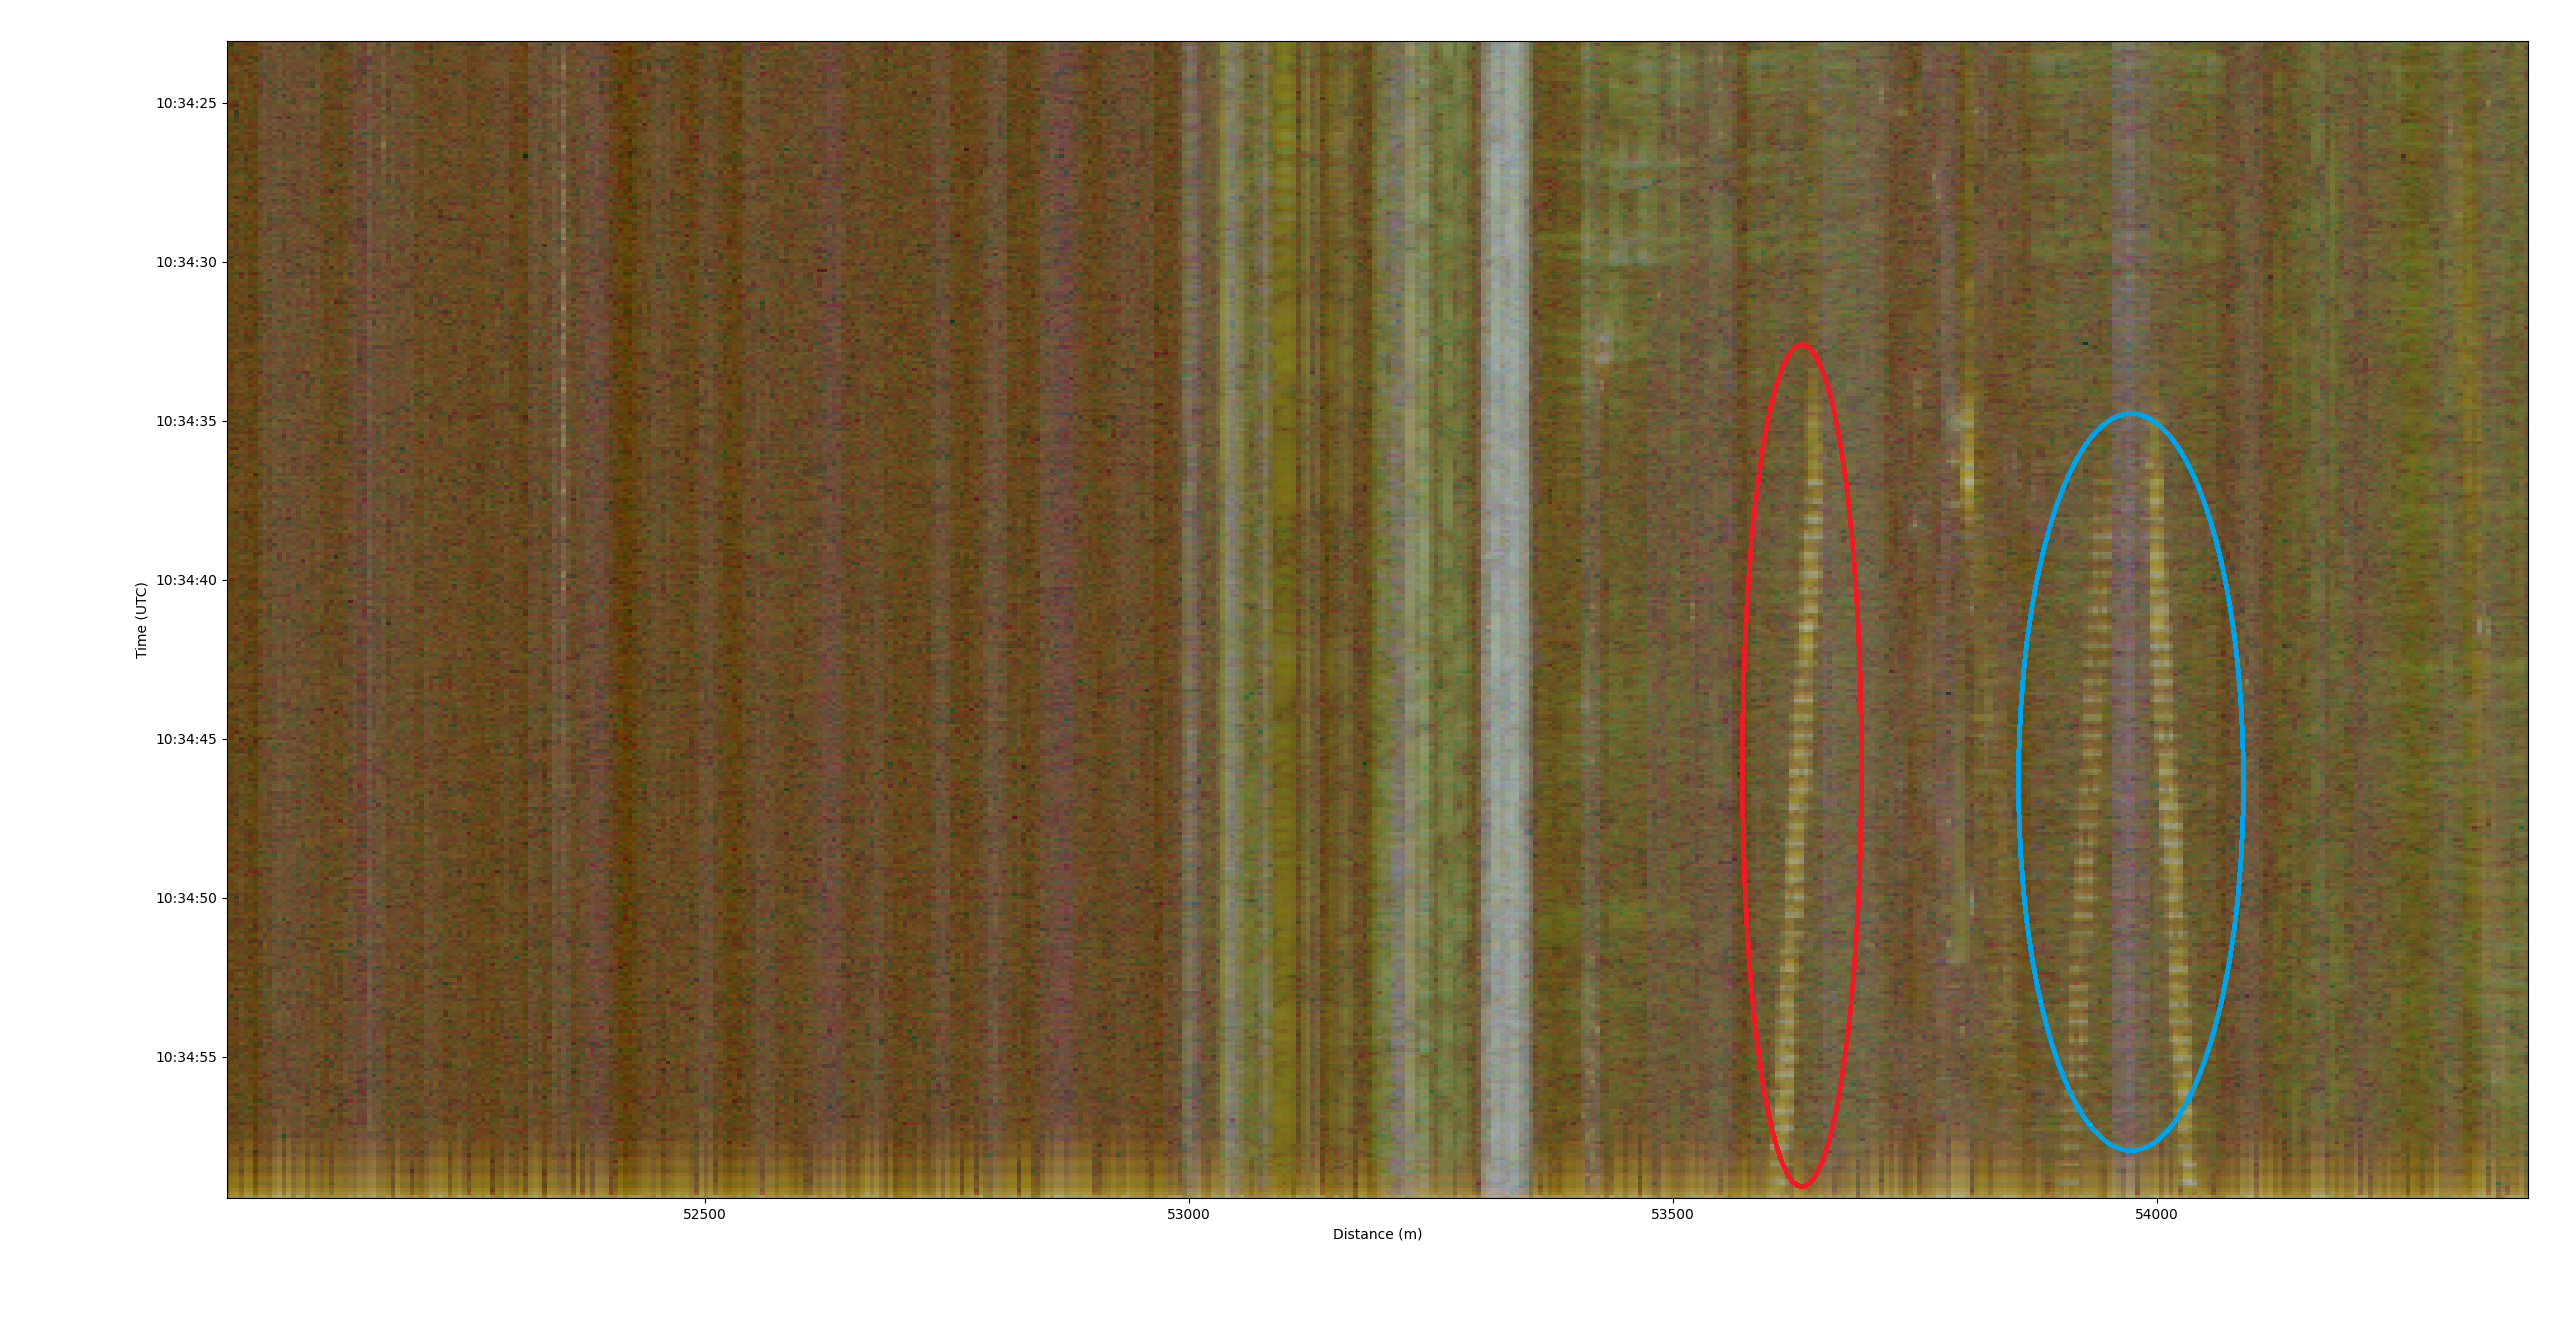
\includegraphics[width=\linewidth]{Bilder/jpg/plot_rgb.png}
    \caption{RGB plot for the phase data}
    \label{phase_plot}
\end{figure}

\subsection{Extraction}
\begin{figure}[ht]
  \centering
  \resizebox{\textwidth}{!}{%%
    \begin{tikzpicture}[
      node distance=1cm and 2cm,
      >=Stealth,
      subblock/.style={
        rectangle,
        draw,
        rounded corners,
        text centered,
        minimum width=2.5cm,
        minimum height=0.8cm,
        font=\scriptsize,
        fill=blue!10,
      },
      container/.style={
        rectangle,
        draw,
        thick,
        rounded corners,
        fill=gray!20,
      }
    ]
      % declare background layer
      \pgfdeclarelayer{background}
      \pgfsetlayers{background,main}

      % internal sub-blocks stacked
      \node[subblock] (hdf5) {HDF5 File};
      \node[subblock, below=of hdf5] (masks) {Region Masks};
      % output block
      \node[subblock, right=of masks] (steps) {Footstep and Background Files};

      % arrows from inputs to output
      \draw[->] (hdf5.east) -- ++(0.5,0) |- (steps.west);
      \draw[->] (masks.east) -- ++(0.5,0) -- (steps.west);

      % container in background
      \begin{pgfonlayer}{background}
        \node[container, fit=(hdf5) (masks) (steps), inner sep=10pt] (extract) {};
        \node[anchor=north west, font=\scriptsize] at (extract.north west) {Extraction};
      \end{pgfonlayer}
    \end{tikzpicture}%%
  }
  \caption{Extraction block: HDF5 file and Region masks are used to extract footstep and background data.}
  \label{fig:extraction_block}
\end{figure}

Figure~\ref{fig:extraction_block} shows the internal structure of extraction block which serves to isolate and package all footstep and background segments for downstream processing. It takes two simple inputs the raw phase data stored in the HDF5 file and the corresponding region masks and produces a set of cleaned, per event files. This abstract view hides the internal annotation details, focusing on the high-level data flow from stored measurements to ready to use footstep files.

\begin{figure}[ht]
  \centering
  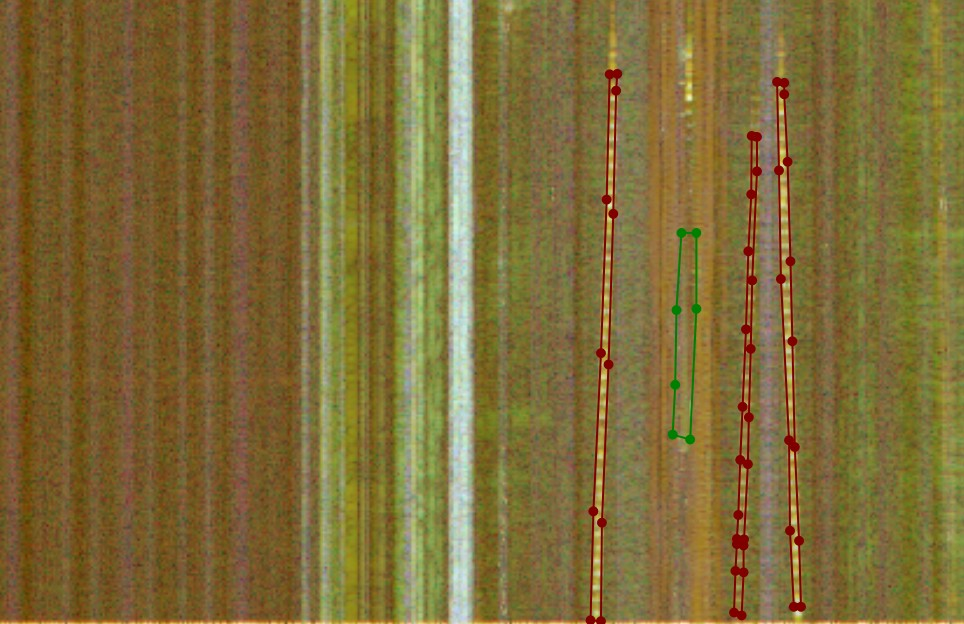
\includegraphics[width=\linewidth]{Bilder/jpg/labelme.jpg}
  \caption{Region annotation of background and footstep data}
  \label{labelme}
\end{figure}
 
Figure~\ref{labelme} shows the region masks for the annotation of the background and footstep data. The green annotation shows the background data and the red annotation shows the footsteps data. These annotations are used to store files in different folders such as background and walking. The annotation is done on the same HDF5 file shown in the Figure~\ref{phase_plot}.   

\subsection{Preprocessing}\label{sec:preprocessing}
The files generated from the extraction block need to be preprocessed in such a way that the footsteps are clearly visible. To help this cause, the preprocessing block converts the extracted files into spectrograms. The spectrograms are generated using the Short-Time Fourier Transform (STFT). Figure~\ref{fig:Preprocessing_block} shows the block diagram of the preprocessing block with all the operations done on the data files to get the spectrograms.

\begin{figure}[ht]
  \centering
  \resizebox{\textwidth}{!}{%%
    \begin{tikzpicture}[
      node distance=1cm,
      >=Stealth,
      subblock/.style={
        rectangle, draw, rounded corners, text centered,
        minimum width=2.5cm, minimum height=0.8cm,
        font=\scriptsize, fill=blue!10,
      },
      container/.style={
        rectangle, draw, thick, rounded corners, fill=gray!20,
      }
    ]
      % layers
      \pgfdeclarelayer{background}
      \pgfsetlayers{background,main}

      % sub-blocks inside
      \node[subblock] (acc) {Accumulator};
      \node[subblock, right=of acc] (stft) {STFT};
      \node[subblock, right=of stft] (spec) {Spectrogram};

        % Draw arrows
      \draw[->] (acc) -- (stft);
      \draw[->] (stft) -- (spec);

      % container background
      \begin{pgfonlayer}{background}
        \node[container, fit=(acc) (stft) (spec), inner sep=10pt] (prep) {};
        \node[anchor=north west, font=\scriptsize] at (prep.north west) {Preprocessing};
      \end{pgfonlayer}
    \end{tikzpicture}%%
  }
  \caption{Preprocessing block: Footstep/Background files are processed through an Accumulator and STFT to produce Spectrograms.}
  \label{fig:Preprocessing_block}
\end{figure}

Extracted data files from the extraction block are passed to the preprocessing block. Accumulator block takes the data files and integrates the phase-difference stream into a continuos phase signal and then the high-pass filters out slow drifts in such a way that only dynamic events like footsteps are visible. The STFT block takes this accumulated phase and converts it into a spectrogram. STFT is a mathematical technique that transforms the time-domain signal into the frequency domain, allowing for the analysis of the signal's frequency content over time. The output of the STFT is a spectrogram which is a visual representation of the signal's frequency content over time. Figure~\ref{walking_1d} shows such spectrogram which is generated from the footsteps data. The spikes seen in the spectrogram are the footsteps which are clearly visible. 

\begin{figure}[h]
  \centering
  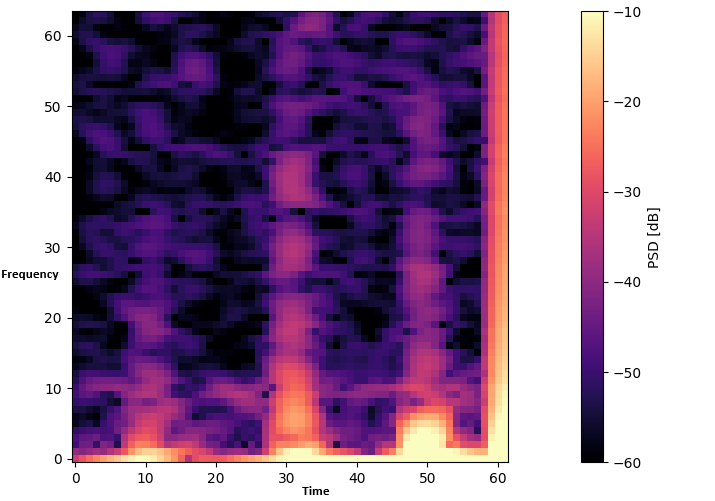
\includegraphics[width=0.7\linewidth]{Bilder/jpg/walking_1d.png}
  \caption{Spectrogram for walking data}
  \label{walking_1d}
\end{figure}

Background noise is also be visualized in the spectrograms in a similar manner. Figure~\ref{bg_1d} shows the spectrogram for background noise data. The spectrograms has no pattern of footsteps here. The pattern of footsteps has spikes but background noise will have a constant pattern which doesn't have distortions. The footsteps will have a significant spikes in the spectrograms unlike the background noise. This is a clear distinction between the footsteps and background noise spectrograms. 

\begin{figure}[h]
  \centering
  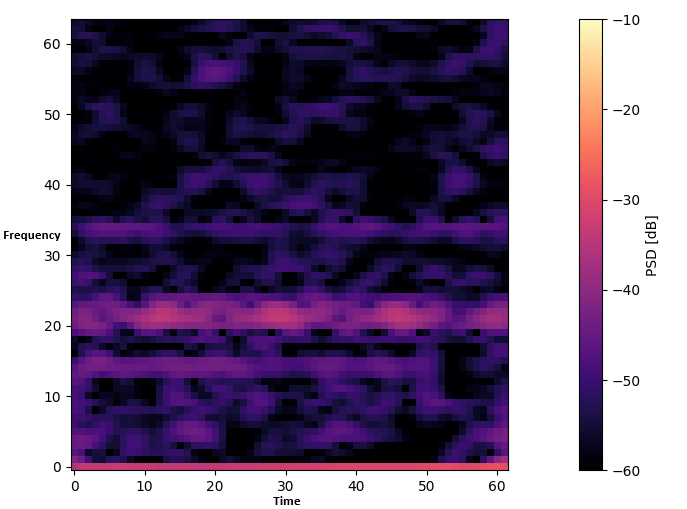
\includegraphics[width=0.7\linewidth]{Bilder/jpg/background_1d.png}
  \caption{Spectrogram for background noise data}
  \label{bg_1d}
\end{figure}

\subsection{Training the model}
Dataset created from the preprocessing block contains the footstep data and background data. Training block takes the dataset and trains the model using the ConvNext V2 and EfficientNet models. Figure~\ref{fig:training_block} shows the block diagram of the training pipeline.
\begin{figure}[ht]
  \centering
  \resizebox{\textwidth}{!}{%%
    \begin{tikzpicture}[
      node distance=1cm and 1.5cm,
      >=Stealth,
      subblock/.style={
        rectangle, draw, rounded corners, text centered,
        minimum width=3cm, minimum height=1cm,
        font=\scriptsize, fill=blue!10,
      },
      container/.style={
        rectangle, draw, thick, rounded corners, fill=gray!20,
      }
    ]
      % layers
      \pgfdeclarelayer{background}
      \pgfsetlayers{background,main}

      % Sub-blocks: first row
      \node[subblock] (dataset) {Dataset};
      \node[subblock, right=of dataset] (split) {Train/Val Split};
      \node[subblock, right=of split] (aug)   {Augmentation};
      % second row
      \node[subblock, below=of aug] (train) {Training};
      \node[subblock, left=of train] (val)   {Validation};
      \node[subblock, left=of val] (ckpt)   {Checkpoint};

      % Arrows
      \draw[->] (dataset) -- (split);
      \draw[->] (split) -- (aug);
      \draw[->] (aug.south) -- (train.north);
      \draw[->] (train) -- (val);
      \draw[->] (val) -- (ckpt);

      % Container background
      \begin{pgfonlayer}{background}
        \node[container, fit=(dataset) (split) (aug) (train) (val) (ckpt), inner sep=10pt] (trainC) {};
        \node[anchor=north west, font=\scriptsize] at (trainC.north west) {Training};
      \end{pgfonlayer}
    \end{tikzpicture}%%
  }
  \caption{Model training block: Footstep/Background dataset is split into training and validation sets, augmented, and then trained and validated.}
  \label{fig:training_block}
\end{figure}

The dataset consists of the spectrograms of footstep and background data. The dataset is split into training and validation sets in the ratio of 80:20. Training set is being applied augmentations to generalize the dataset so the model learns the features of the dataset and not memorize the dataset. The augmentations are explained in the section~\ref{sec:augmentation}. Training set is then passed to the model for training. Model is validated by just passing the validation set to the model. Model is trained and the checkpoint is saved. Checkpoint is the model weights which are saved after every epoch The model is then tested using the test set which is not used for training or validation. Test set is used to evaluate the performance of the model. Test set is passed to the model and the accuracy of the model is calculated using the checkpoint saved during the training. Testing follows the same process as validation, but done on the test set.  

% ==================================
% ==================================
%  Kapitel 4 - Mathematische Formeln
% ==================================
% ==================================


\chapter{Implementation}
\label{ch:implementation}

In this chapter, we move from system design (Chapter~\ref{sec:system_design}) to the concrete realization of our pipeline.  We detail how each component was implemented in practice from data extraction from the HDF5 files using region masks and custom scripts to signal preprocessing for spectrogram generation culminating in model training with various data augmentation techniques and checkpointing. Discussion on how the specific libraries and frameworks adopted, the structure of key code modules, configuration parameters, and the strategies employed to validate and manage intermediate outputs, providing a clear, end-to-end account of how the system was built, tuned, and prepared for deployment.  


\section{Extraction of Footstep and Background Data}
Data collected from the setup explained in section~\ref{sec:experimental_setup} is stored in the HDF5 file. HDF5 file is visualized as explained in section~\ref{sec:data_acquisition} and shown in Figure~\ref{phase_plot}. Region masks are used to extract the footstep and background with the help of annotations on RGB plot of the HDF5 file. RGB plot is used to enhance the visual interoperability, for which a Short-Time Fourier Transform (STFT) in tandem with a custom-designed filter bank. The application of a logarithmic transformation further enhances the visualization, making subtle patterns more evident. Figure~\ref{labelme} provides an illustrative RGB image of the raw phase data where the horizontal axis corresponds to the distance along the cable route and the vertical axis represents time, with time progressing from the top (earliest) to the bottom (latest). The RGB plot is opened using the LabelMe tool. 

\begin{figure}[h]
    \centering
    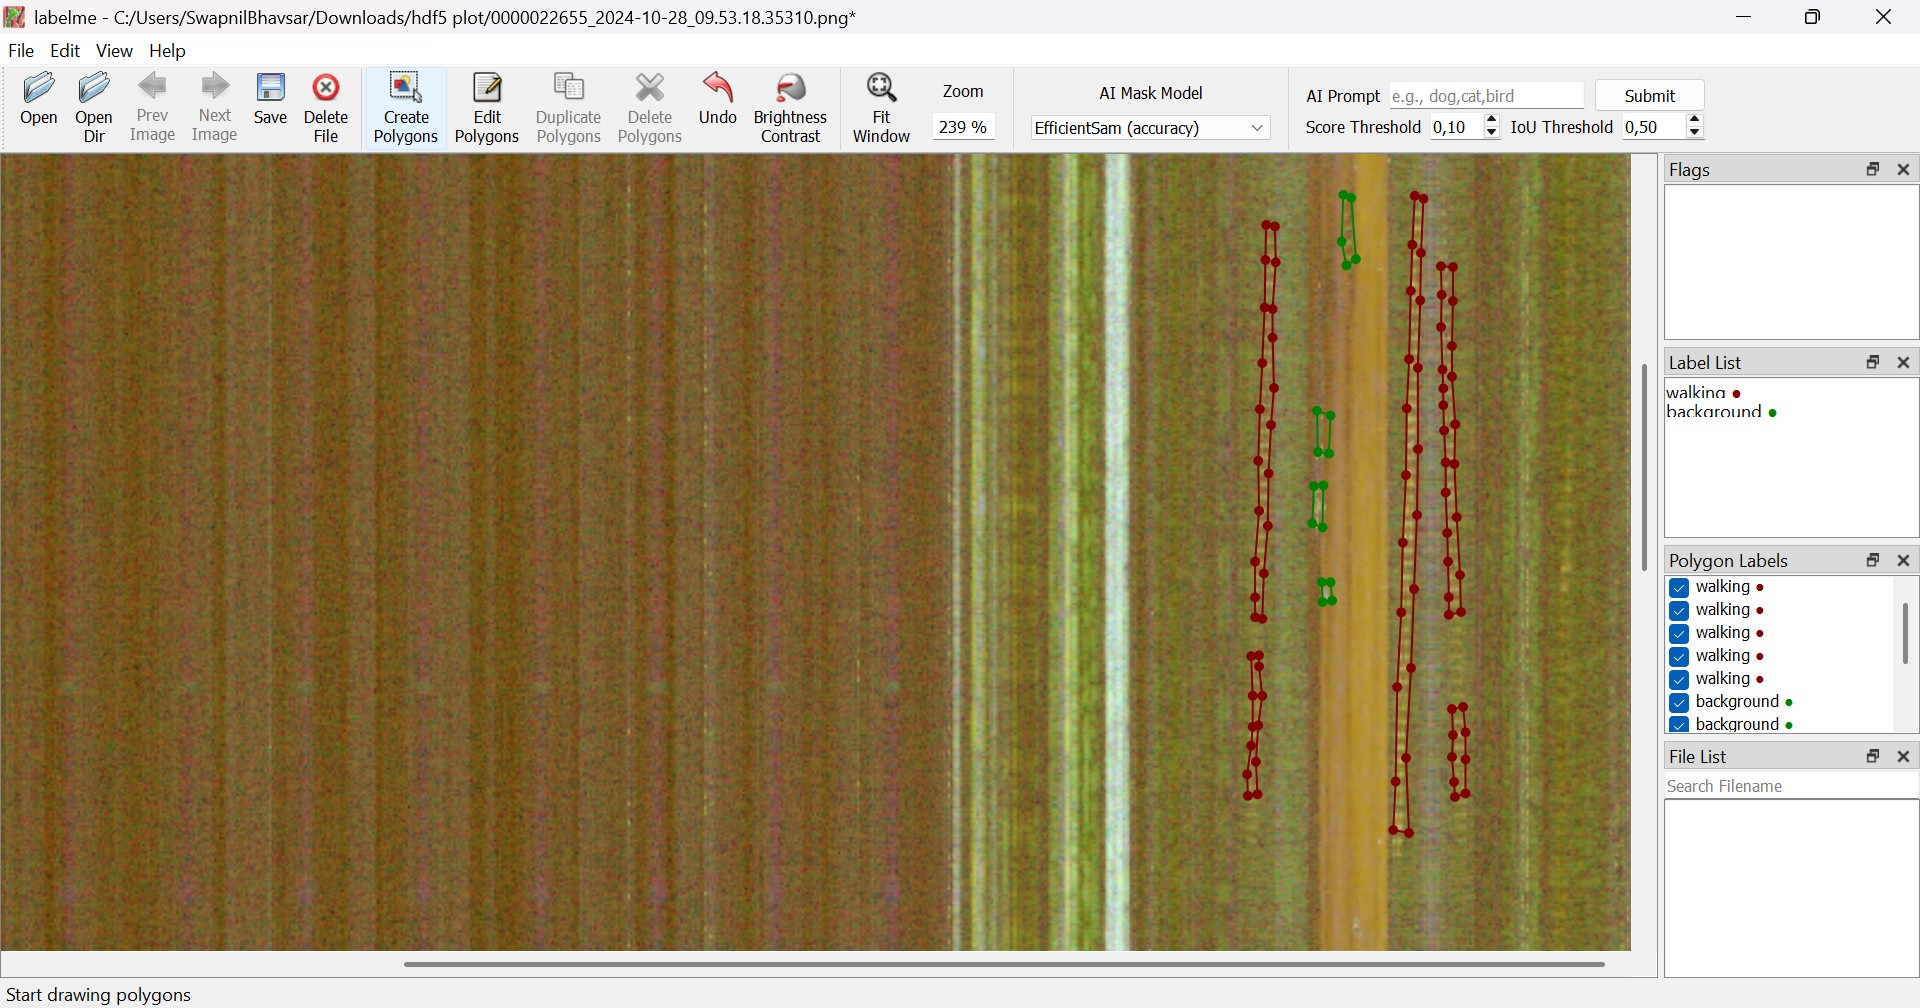
\includegraphics[width=\linewidth]{Bilder/jpg/label.jpg}
    \caption{LabelMe tool for annotation}
    \label{labelme}
\end{figure}

RGB plot has footsteps trails in it and we need to annotate it and extract the footsteps data using the RGB plot and HDF5 files. LabelMe tool is used to annotate the footsteps trail in RGB plot. LabelMe tool is a open-source image annotation tool that allows users to draw polygons on images and generate JSON files containing the binary masks corresponding to the annotated regions. The class labels are also added to the annotated regions. The extraction blocks takes the JSON masks and the HDF5 file which is used to extract the footstep data from the HDF5 file and store it in .npy or .bin file~\cite{Labelme}. Figure~\ref{labelme} shows the window for the LabelMe tool. It contains a RGB plot for HDF5 file. It contains option to draw the polygons for the exact part which is needed for the dataset. Figure~\ref{labelme} has two different colors of polygons where red polygon is used to annotate footstep data and the green polygon is used to annotate the background data.

The output from Labelme includes JSON files, which contain binary masks corresponding to the annotated regions. A custom script is then used to extract the appropriate raw phase data segments from the HDF5 files by applying the binary masks. Listing~\ref{lst:core_extraction} presents the core function that embodies the sample extraction process.

\begin{lstlisting}[style=pythonstyle, caption={Core logic for extracting samples from a mask}, label=lst:core_extraction]
def extract_samples_from_mask(mask, data_array, data_rate_hz, 
                    window_len_sec, window_width_channels):
    window_length_traces = int(data_rate_hz * window_len_sec)
    hop_size_time = int(window_length_traces * 0.5)
    hop_size_space = max(1, int(window_width_channels * 0.5))
    
    actual_mask = mask[::-1]
    col_has_label = np.any(mask, axis=0)
    row_has_label = np.any(mask, axis=1)
    left_start = np.argmax(col_has_label)
    right_end = len(col_has_label) - np.argmax(col_has_label[::-1])
    top_start = _DOWNSAMPLE_FACTOR * np.argmax(row_has_label)
    bottom_end = _DOWNSAMPLE_FACTOR * (len(row_has_label) - np.argmax(row_has_label[::-1]))
    
    for start_x in range(max(0, left_start - hop_size_space), 
                            right_end - hop_size_space, hop_size_space):
        for start_y in range(max(0, top_start - hop_size_time), 
                             bottom_end - hop_size_time, hop_size_time):
            chunk = data_array[start_y : start_y + window_length_traces, 
                                start_x : start_x + window_width_channels]
            mask_chunk = actual_mask[start_y // _DOWNSAMPLE_FACTOR : 
                                    (start_y + window_length_traces) // _DOWNSAMPLE_FACTOR,
                                    start_x : start_x + window_width_channels]
            if chunk.shape != (window_length_traces, window_width_channels) or \
                np.mean(mask_chunk.astype(float)) < _REQUIRED_MASK_PROPORTION:
                continue
    \end{lstlisting}

In this function, several key computational steps are performed:
    \begin{itemize}
        \item The window length is calculated based on the data rate and the desired duration.
        \item A binary mask, generated from Labelme annotations, is processed to identify the columns and rows that contain labels.
        \item Nested loops are implemented to extract segments of the raw phase data along both spatial and temporal dimensions.
        \item The extracted segments, referred to as \texttt{chunk} and \texttt{mask\_chunk}, are then verified based on their shape and the proportion of the label mask present before being stored for further processing.
    \end{itemize}

The extracted files (.npy/.bin files) are stored in different directories based on the type of data (footstep or background) and the corresponding labels. Based on the labels, the data is divided into training and test sets. 
These sets are preprocessed before being used for training and testing the model. 

\section{Preprocessing of extracted Data}
\label{preproc}
Following extraction, the extracted files needs to be preprocessed so that the clear distinction between the footsteps and background data can be made. The distinction is seen in the form of spikes which is visible in footstep data in comparison to background data as seen in Figure~\ref{walking_1d} and Figure~\ref{bg_1d} from section~\ref{sec:preprocessing}.  The preprocessing is used to convert the raw phase data into a more interpretable format, specifically a spectrogram. This transformation is crucial for the subsequent training of the model, as it allows for the identification of patterns and features that are indicative of footstep events. The preprocessing pipeline is designed to handle the raw phase data efficiently, ensuring that the resulting spectrograms are both informative and suitable for machine learning applications. We use Scipy's signal tools~\cite{scipy2020} for filtering and STFT, torchaudio's Mel-scale filter banks~\cite{torchaudio2024}.

The preprocessing routine, as demonstrated in Listing~\ref{lst:mag_processing}, involves reading the extracted data files, executing the STFT, and finally converting the resulting power spectrum into decibel (dB) values. The transformation to a logarithmic scale is critical, as it optimizes the dynamic range of the visualized data and makes both prominent and subtle patterns more discernible. We employ the \texttt{Visualizer} class which is the custom created class for these operations in the listing~\ref{lst:mag_processing}. In its constructor we build a Mel-filter bank matrix via \texttt{melscale\_fbanks(...,~mel\_scale="htk",...)}, which yields finer resolution at low frequencies where footstep energy is concentrated and coarser resolution at high frequencies, improving both compactness and interpretability of the spectrogram. The method \texttt{\_accum} prepares raw data by taking a cumulative sum and then applying a high-pass filter to remove low-frequency drift. Finally, \texttt{preprocess} computes the STFT, squares the magnitude, and applies a $10\log_{10}(\cdot)$ transform to produce the final spectrogram. The logarithimic function make the spectrograms both visually clearer and more suitable to downstream classification. 

\begin{lstlisting}[style=pythonstyle, caption={Core processing for converting raw phase data to magnitude output}, label=lst:mag_processing]
class Visualizer:
   def __init__(self, data_rate_hz: int = 1000):
        self._data_rate_hz = data_rate_hz
        self._f_bank = (
            melscale_fbanks(
                n_freqs= 128 // 2 + 1,
                f_min=0,
                f_max=500,
                n_mels=64,
                sample_rate=data_rate_hz,
                mel_scale="htk",
                norm=None,
            )
            .cpu()
            .numpy()
        )

    def _accum(self, x: np.ndarray) -> np.ndarray:
        x = np.cumsum(x, axis=0, dtype=np.int64).astype(np.float32)*INT_TO_RADIANS
        sos = signal.butter(2, 5, "hp", fs=1000, output="sos")
        return signal.sosfiltfilt(sos, x, axis=0)

    def preprocess(self, data: np.ndarray) -> np.ndarray:
        data_accum = np.cumsum(data, axis=0)
        f, t, stft = signal.stft(
            data_accum, fs=self._data_rate_hz,
            nperseg=128, noverlap=114,
            padded=False, scaling="psd", axis=0
        )
        stft = np.abs(stft) ** 2
        stft = np.matmul(stft.T, self._f_bank).T
        mag = 10 * np.log10(stft)
        return mag
\end{lstlisting}

To facilitate the training of the deep learning models such as ConvNext V2 and EfficientNet. Two different models are trained so that a comparison can be made for their performances and accuracies, two separate datasets are generated through variations in the sample length and the number of spatial channels considered:
\begin{itemize}
    \item The first dataset employs a sample length of 1.728 seconds and uses only 1 spatial channel. Sample length of 1.728 seconds as it contains 3 to 4 steps and the dataset with same configuration as there are already recorded files available. Based on the models trained on these, it is useful to detect shorter as well as longer footstep trails. The processing pipeline for this dataset is executed using the extraction procedure from Listing~\ref{lst:core_extraction} and is subsequently converted into spectrograms following the process described in Listing~\ref{lst:mag_processing}. Figure~\ref{walking_1ch} illustrates the resulting spectrogram for walking data acquired through a single spatial channel. In this Figure, the upper plot corresponds to the phase plot which reveals the unwrapped phase variations over time, whereas the lower plot represents the corresponding STFT spectrogram. Noticeably, the distinct spikes present in the spectrogram mark the precise moments when a foot makes contact with the ground.
    
    \begin{figure}[h]
        \centering
        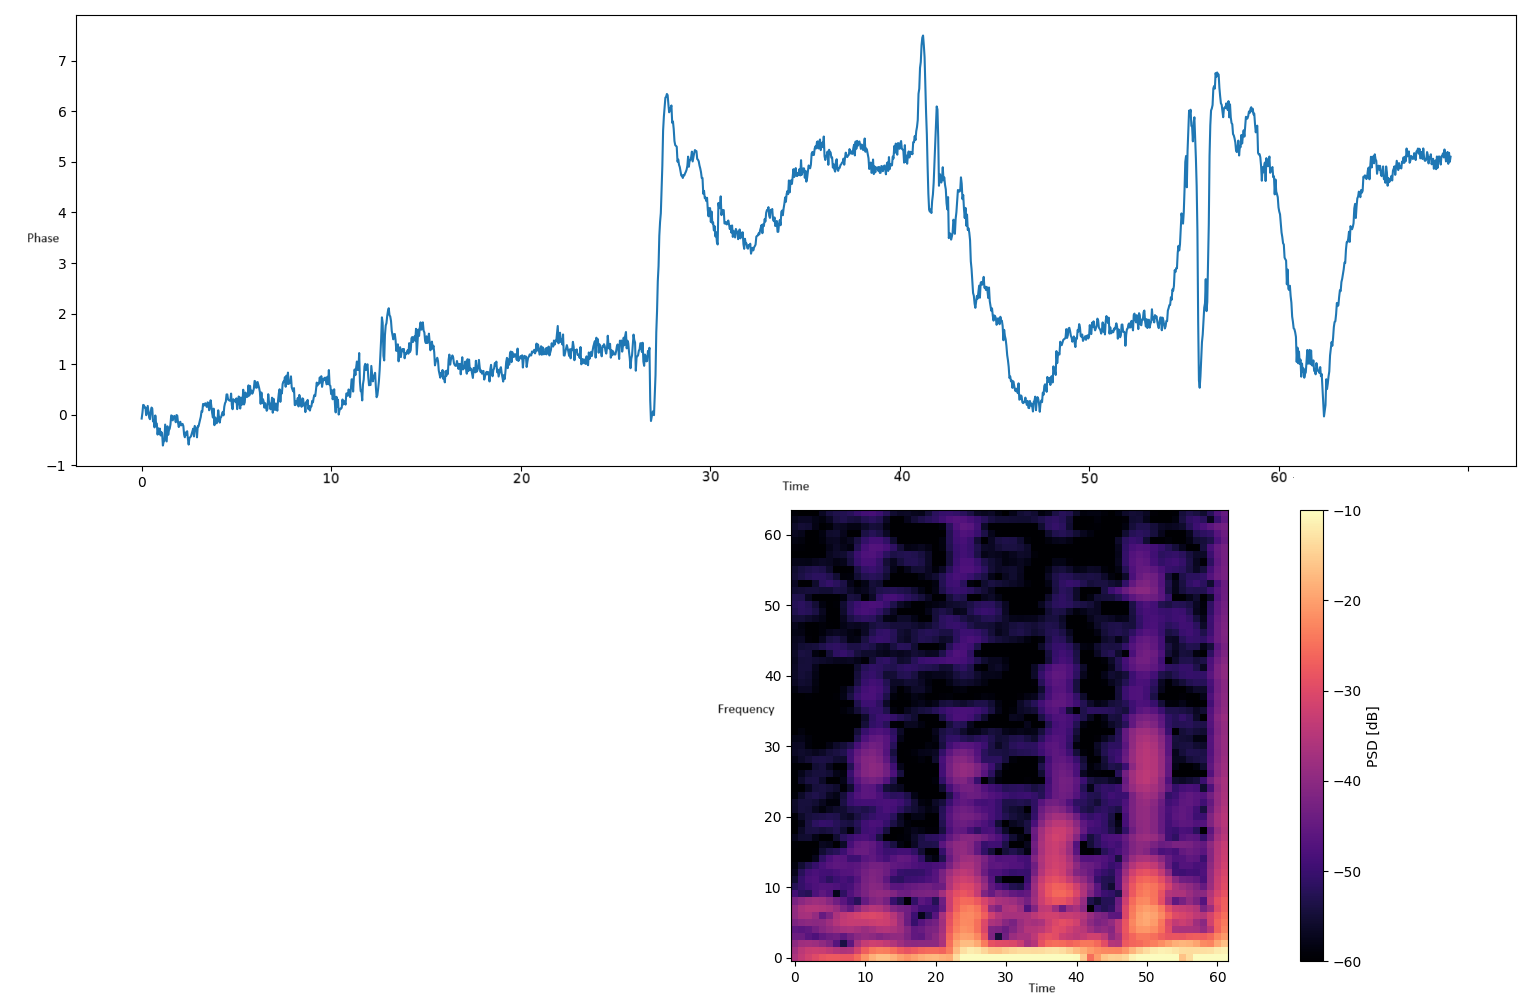
\includegraphics[width=0.8\linewidth]{Bilder/jpg/walking_1ch.png}
        \caption{Spectrogram for walking data with 1 spatial channel}
        \label{walking_1ch}
    \end{figure}

    \item The second dataset is designed for capturing more complex spatial and temporal interactions and uses a sample length of 2 seconds along with 10 spatial channels. The sample length of 2 seconds is taken which can be estimated as the time length in which a person can take 3 to 4 steps. The spatial channels record the data which are 5m apart. So the neighboring spatial channels record distortions based on the same footsteps and they can be detected many times by trained model. To avoid this 10 spatial channel are selected so model can exactly focus on footsteps and not the distortions in the neighboring spatial channels. The same extraction and preprocessing techniques are applied to this dataset. Figure~\ref{walking_10ch} shows that the top plot represents the distribution of the spatial channels over time, while the bottom plot highlights the frequency distribution. Importantly, files that lack clearly discernible footsteps are manually filtered out, ensuring that the final dataset is diverse and rich in footstep patterns. This deliberate filtering is paramount as it enhances the model's ability to generalize across various walking patterns and substantially reduces the occurrence of false detections.
\end{itemize}

\begin{figure}[h]
    \centering
    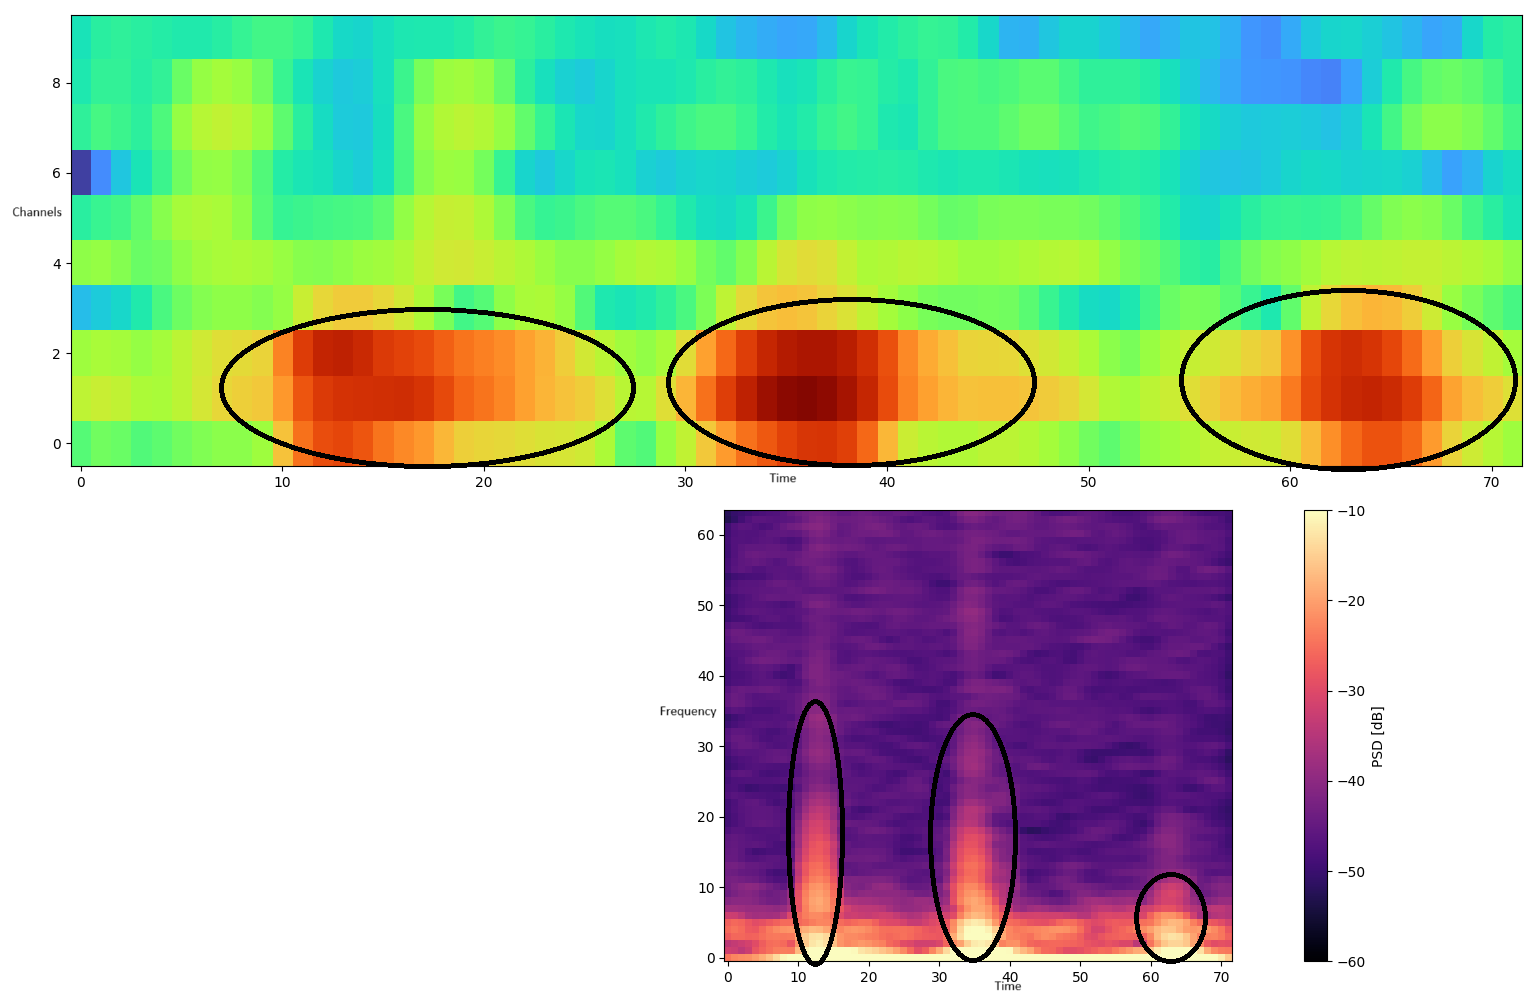
\includegraphics[width=0.8\linewidth]{Bilder/jpg/walking_10ch.png}
    \caption{Spectrogram for walking data with 10 spatial channels}
    \label{walking_10ch}
\end{figure}

\section{Dataset}
\label{sec:dataset}
The dataset is created with the help of preprocessing steps. The raw extracted files (.npy/.bin) are stored in the folder and before the dataset is loaded to train the model, the preprocessing steps are used. Dataset are of two types as described in the section~\ref{preproc}.

\begin {itemize}
\item \texttt{Dataset-1D}: 1.728 seconds sample length and 1 spatial channel
\item \texttt{Dataset-2D}: 2 seconds sample length and 10 spatial channels
\end {itemize}

Both datasets contains the \texttt{training} and \texttt{testing} folders which are used for the same purpose as the name suggests. Each of these folders has two folders \texttt{walking} and \texttt{background} which are different events that are used as labels for training the models.

\texttt{Dataset-1D} training folder 5818 walking samples and 2696 background samples. Testing folder for the same dataset contains 988 walking samples and 1590 background samples. \texttt{Dataset-2D} contains the same folders as \texttt{Dataset-2D} where training folder contains 1982 walking samples and 421 background samples. Testing folder contains 65 walking samples and 1682 bakcground samples.

\texttt{Dataset-2D} has much lesser samples compared to \texttt{Dataset-1D} because over the same HDF5 files the samples are created using 10 spatial channels. So in \texttt{Dataset-2D} the one sample consists of 10 samples clubbed together from \texttt{Dataset-1D}. 
  
\section{Training and Validation of the Model}
The training of the model is done using the PyTorch framework~\cite{PyTorch_website}. Pytorch framework has rich ecosystem of libraries like which helps is leveraging of the models ConvNext V2 and EfficientNet from \texttt{timm}~\cite{rw2019timm}. The dataset made with the help of preprocessing is used to train the model. The extracted data in the dataset folders is augmented using the different augmentation processes. Numpy arrays given out by the preprocessing function in listing~\ref{lst:mag_processing}. As the model requires the tensor input, the numpy arrays are converted to tensors using the \texttt{torch.from\_numpy} function. All the further steps before inputting the data to the model are carried out using the tensors. Normalization of the data is a very important step which is done before inputting the data to the model. The tensors for the case are not actually the image tensors so the mean and standard deviation are calculated for the spectrograms which are used for the normalization. Listing~\ref{lst:data_reading_stats} shows the code for reading the data files and computing the mean and standard deviation. The folder path with all the data files(training and testing both) is given to the function \texttt{read\_files\_from\_folder} which reads the data files and gives it the visualizer class that contains the function for spectrogram preprocessing shown in the Section~\ref{sec:preprocessing}. All the values are stacked together and given to the function \texttt{calculate\_mean\_std} which calculates the mean and standard deviation of the data. These mean and standard deviation values are used for the normalization of the data.

\begin{lstlisting}[style=pythonstyle, caption={Reading data files and computing dataset statistics}, label=lst:data_reading_stats]
    def read_files_from_folder(folder_path: Path):

        all_data = []
        viz = Visualizer()
    
        for file_path in folder_path.rglob("*"):
            if file_path.suffix == ".bin":
                with open(file_path, "rb") as f:
                    data = np.fromfile(f, dtype=np.int64)
                data = data.reshape((length, channels))
            elif file_path.suffix == ".npy":
                data = np.load(file_path)
            else:
                continue
    
            stft_data = viz.data_process(data)
            all_data.append(stft_data)
    
        if not all_data:
            raise ValueError(f"No valid data files found in {folder_path!r}.")
    
        stacked_data = np.stack(all_data, axis=0)
        return stacked_data
    
    
    def calculate_mean_std(data):
        tensor_data = torch.from_numpy(data.astype(np.float32))
        mean = torch.mean(tensor_data)
        std = torch.std(tensor_data)
        return mean, std
    \end{lstlisting}

Augmentation processes are used to increase the size of the dataset and to make the model robust. The augmentation techniques for images are explained in Section~\ref{sec:augmentation}. Similar augmentation techniques are applied to the spectrograms. Augmentations are not applied to all the files instead based on the probability it is applied randomly on the files before giving it to model. Some augmentations come from the module augmentation from the predefined library Kornia, while others are custom made (Listing~\ref{lst:custom_augmentations}).  Below is a summary of each custom augmentation class:

\begin{lstlisting}[style=pythonstyle, caption={Custom data augmentation modules}, label=lst:custom_augmentations]
    class RandomAffineHorizontalScalePyTorch(torch.nn.Module):
        def __init__(self, scale=1.1, p=0.5):
            super().__init__()
            self.scale = scale
            self.p = p
            
        def forward(self, img: torch.Tensor) -> torch.Tensor:
            if torch.rand(1).item < self.p:
                N, C, H, W = img.shape
                theta = torch.tensor([[[self.scale, 0, 0],
                                       [0, 1.0,    0]]] * N,
                                     dtype=img.dtype,
                                     device=img.device)
                grid = F.affine_grid(theta, img.size(), align_corners=False)
                img = F.grid_sample(img, grid, align_corners=False)
            return img
    
    
    class RandomAmplitudeScaling:
        def __init__(self, scale_range=(0.9, 1.1)):
            self.scale_range = scale_range
        
        def __call__(self, tensor: torch.Tensor) -> torch.Tensor:
            factor = torch.empty(1).uniform_(*self.scale_range).item()
            multiplier = torch.ones(tensor.size(2), device=tensor.device) * factor
            multiplier = multiplier.view(1, 1, -1, 1)
            return tensor * multiplier
    
    
    class RandomGaussianNoise:
        def __init__(self, mean=0.0, std=1.0, p=0.5):
            self.mean = mean
            self.std = std
            self.p = p  
    
        def __call__(self, tensor: torch.Tensor) -> torch.Tensor:
            if torch.rand(1).item() < self.p:
                noise = torch.randn_like(tensor) * self.std + self.mean
                tensor = tensor + noise
            return tensor
    \end{lstlisting}

Explaination of what and every augmentation does to the dataset is as follows:
\begin{itemize}
    \item \texttt{RandomAffineHorizontalScalePyTorch}:\\
      Randomly stretches each spectrogram horizontally by~$\pm10\%$. In the demonstration (Figure~\ref{aug}), this warp reduces three peaks to two, making the effect clearly visible. This helps the model generalize to variations in footstep segment length when recordings are truncated or extended.
  
    \item \texttt{RandomAmplitudeScaling}:\\
      Multiplies the spectrogram tensor by a random factor in the interval~$[0.9,1.1]$, varying its amplitude by up to~$\pm10\%$ making the signals weaker or stronger. In the demo we used a fixed factor of~1.5, so the darker peaks in the output illustrate this boost in intensity. This accounts for footsteps with weaker or stronger signal strengths.
  
    \item \texttt{RandomGaussianNoise}:\\
      Injects additive Gaussian noise (with mean and standard deviation calculated from the dataset) into the spectrogram. The resulting graininess ("pixelation") in the visualization reflects this perturbation, improving robustness to sensor and environmental noise.
  
    \item \texttt{kornia.augmentation.Normalize~\cite{kornia}}:\\
      Standardizes the spectrogram tensor using its computed mean and standard deviation (Listing~\ref{lst:data_reading_stats}), ensuring a consistent dynamic range for model inputs. You can see the changed value range compared to the raw input.
  
    \item \texttt{kornia.augmentation.RandomHorizontalFlip~\cite{kornia}}:\\
      Flips the spectrogram horizontally, augmenting the dataset by mirroring temporal patterns so the model learns footstep patterns in both forward and reverse temporal order.
  \end{itemize}

Each augmentation's application is gated by \texttt{if torch.rand(1).item() < self.p:} which cleanly compares a Python float to the probability \texttt{p}, ensuring a defined chance of applying each transform.

\begin{figure}[h]
    \centering
    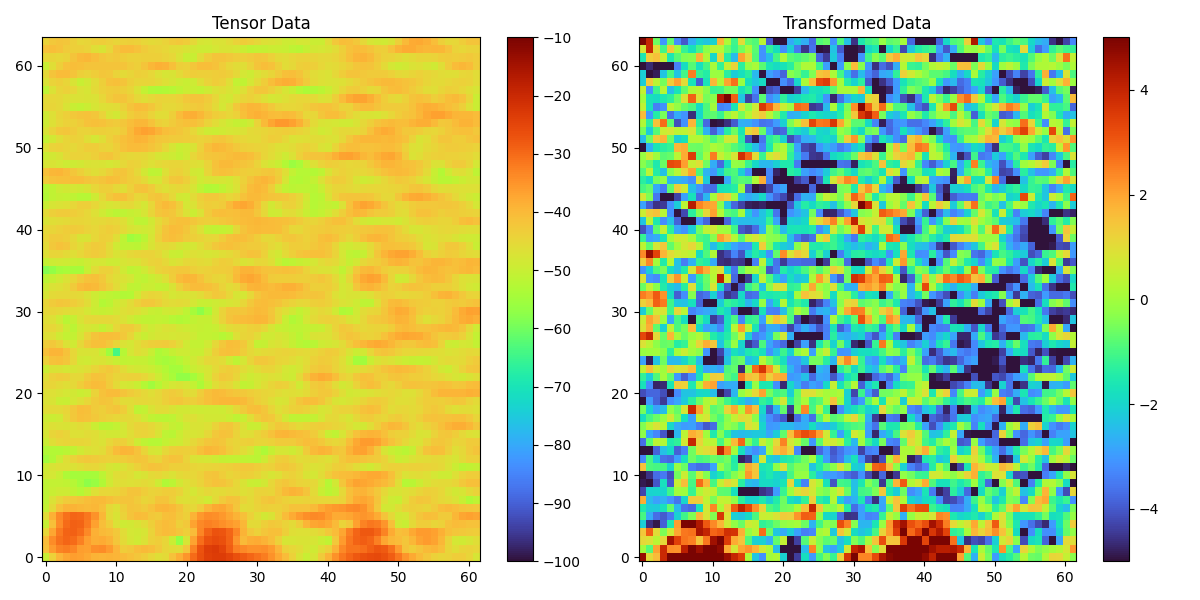
\includegraphics[width=\linewidth]{Bilder/jpg/aug.png}
    \caption{Augmentations of the input tensor}
     \label{aug}
\end{figure}

Figure~\ref{aug} shows the implementation of the augmentation on the input tensor. Augmentations are enhanced for the sake of demonstration. Summarization of each augmentation applied on the data is as follows:
  
These transformations are applied in the custom dataset loader shown in Listing~\ref{lst:binfile_dataset}. PyTorch's recommended pattern is followed for creating a custom dataset from the documentation on PyTorch's website \cite{PyTorch_website}, which allows seamless integration with \texttt{DataLoader} and other utilities. The constructor takes a root directory containing subfolders named after each class (in our case, \texttt{walking} and \texttt{background}), and it builds internal lists of file paths and corresponding integer labels. The \texttt{\_\_len\_\_} method reports the total number of files (i.e.\ the number of samples per epoch), while \texttt{\_\_getitem\_\_} loads each file, applies the STFT-based processing, permutes axes to match PyTorch's \texttt{(C, H, W)} convention, and if a \texttt{transform} is provided it runs the custom augmentations before returning the \texttt{(tensor, label)} pair. This structure cleanly separates I/O, signal preprocessing, and augmentation, making the training loop straightforward.  

\begin{lstlisting}[style=pythonstyle, caption={Custom Dataset for loading and processing footstep files}, label=lst:binfile_dataset]
    class BinFileDataset(Dataset):
        def __init__(self, root_dir: str, event_types: Dict[int, Union[str, List[str]]], transform=None):
            self.root_dir = Path(root_dir)
            self.transform = transform
    
            # labels
            self.event_types = event_types
            self.class_to_idx = {cls_name: idx for idx, cls_name in event_types.items()}
            self.file_list = []
            self.labels = []
    
            self.visualizer = Visualizer()
            for event_idx, event_type in event_types.items():
                subfolders = [event_type] if not isinstance(event_type, list) else event_type
                for subfolder in subfolders:
                    cls_dir = self.root_dir / subfolder
                    if not cls_dir.exists():
                        raise ValueError(f"Subfolder {cls_dir} does not exist.")
                    for file_path in cls_dir.rglob("*"):
                        if file_path.suffix in [".bin", ".npy"]:
                            self.file_list.append(file_path)
                            self.labels.append(event_idx)
            if not self.file_list:
                raise ValueError(f"No data found in {self.root_dir!r}.")
    
        def __len__(self):
            return len(self.file_list)
    
        def __getitem__(self, idx):
            file_path = self.file_list[idx]
            label = int(self.labels[idx])
            if label < 0 or label >= len(self.event_types):
                raise ValueError(f"Invalid label {label} for file {file_path}.")
    
            if file_path.suffix == ".bin":
                with open(file_path, 'rb') as f:
                    data = np.fromfile(f, dtype=np.int64).reshape((length, channels))
            elif file_path.suffix == ".npy":
                data = np.load(file_path)
            else:
                raise ValueError(f"Unsupported file format: {file_path.suffix}")
    
            tensor_data = self.visualizer.data_process(data)
            tensor_data = torch.from_numpy(tensor_data.astype(np.float32)).contiguous()
            tensor_data = tensor_data.permute(1,0,2).contiguous()
    
            if self.transform:
                transformed_data = self.transform(tensor_data)
                return transformed_data, label
            return tensor_data, label
\end{lstlisting}

The \texttt{BinFileDataset} class wraps the extracted data files into an iterable PyTorch dataset, making it easy to load and preprocess samples on the fly.  In Listing~\ref{lst:training_setup}, definition of two event types (\texttt{walking} and \texttt{background}) in the \texttt{event\_types} dictionary is passed to \texttt{BinFileDataset} along with the root data path. Then splitting the resulting dataset into training and validation subsets using an 80/20 split; a \texttt{deepcopy} of the validation set ensures that training time augmentations do not leak into validation.  All custom augmentations (Listing~\ref{lst:custom_augmentations}) plus normalization are applied to the training split, whereas the validation split only undergoes normalization with the precomputed mean and standard deviation.  Each split is wrapped in a \texttt{DataLoader} (with specified \texttt{batch\_size} and \texttt{num\_workers}) to handle batching and parallel I/O.

For the model, we use the \texttt{timm} library to instantiate a backbone network  (\texttt{effici\allowbreak-entnet\_b0.ra\_in1k} or \texttt{convnextv2\_atto.fcmae\_ft\_in1k}) with pretrained weights, specifying the correct number of output classes and input channels. To address class imbalance, we compute per class weights via \texttt{compute\_class\_weight} from scikit learn library  and supply them to a weighted \texttt{CrossEntropyLoss}, which produces per sample losses.  Finally, we optimize the model using the \texttt{Adam} optimizer (adaptive moment estimation) and log training metrics (loss, accuracy, etc.) to TensorBoard via \texttt{SummaryWriter}.

\begin{lstlisting}[style=pythonstyle, caption={Dataset setup and model initialization }, label=lst:training_setup]
    # Define event labels
    event_types = {0: "background", 1: "walking"}
    
    # Create dataset and split
    dataset = BinFileDataset(root_dir='path/to/data', event_types=event_types)
    train_size = int(0.8 * len(dataset))
    val_size   = len(dataset) - train_size
    train_ds, val_ds = random_split(dataset, [train_size, val_size])
    val_ds = deepcopy(val_ds)
    
    # Assign transforms
    train_ds.dataset.transform = transforms.Compose([
        K.Normalize(mean=channel_means, std=channel_stds),
        K.RandomHorizontalFlip(p=1),
        RandomGaussianNoise(mean=0, std=1.5),
        RandomAmplitudeScaling((0.9, 1.1)),
        RandomAffineHorizontalScalePyTorch(scale=0.7, p=1),
    ])
    val_ds.dataset.transform = transforms.Compose([
        K.Normalize(mean=channel_means, std=channel_stds),
    ])
    
    # DataLoaders
    train_loader = DataLoader(train_ds, batch_size=32, num_workers=8, shuffle=True)
    val_loader   = DataLoader(val_ds,   batch_size=32, num_workers=8, shuffle=False)
    
    # Model, loss & optimizer
    model = timm.create_model("efficientnet_b0.ra_in1k", pretrained=True,
                              num_classes=2, in_chans=1).to(device)
    
    weights = compute_class_weight("balanced", classes=np.unique(all_labels), y=all_labels)
    criterion = nn.CrossEntropyLoss(weight=torch.tensor(weights).to(device))
    optimizer = optim.Adam(model.parameters(), lr=1e-4, weight_decay=1e-2)
    \end{lstlisting}

The other important function used before training is \texttt{mixup\_data}, which implements the MixUp augmentation strategy. It samples a mixing coefficient $\lambda \sim \mathrm{Beta}(\alpha,\alpha)$, shuffles each batch, and forms convex combinations of both inputs and labels. Listing~\ref{lst:mixup_data} shows its implementation. During training, the loss is computed as  
\[
\mathcal{L}
= \lambda\,\ell\bigl(f(\widetilde x),y_a\bigr)
+ (1-\lambda)\,\ell\bigl(f(\widetilde x),y_b\bigr),
\]
encouraging smoother decision boundaries and improved generalization.
\begin{lstlisting}[style=pythonstyle, caption={MixUp data augmentation function}, label=lst:mixup_data]

    def mixup_data(x, y, alpha=0.2):
        if alpha > 0:
            lam = np.random.beta(alpha, alpha)
        else:
            lam = 1.0
        batch_size = x.size(0)
        index = torch.randperm(batch_size).to(x.device)
        mixed_x = lam * x + (1 - lam) * x[index]
        y_a, y_b = y, y[index]
        return mixed_x, y_a, y_b, lam
    \end{lstlisting}


The training loop in Listing~\ref{lst:train_loop} runs for a fixed number of epochs. At the start of each epoch, the model is set to training mode and the running loss and accuracy meter are reset. For each mini-batch, inputs and labels are moved to the GPU, mixed via MixUp (producing \texttt{targets\_a}, \texttt{targets\_b}, and \texttt{lam}), and passed through the network. The combined MixUp loss is computed, backpropagated, and the Adam optimizer updates the weights. Accumulation of batch losses and updating the training accuracy meter is done, then computation and logging the average training loss and accuracy to TensorBoard.

After training, model is switched to evaluation and gradients are disabled. Looping over the validation loader, computing over the standard cross-entropy loss per batch, updating the validation accuracy meter, and accumulating losses is done. At epoch end, the average validation loss and accuracy are computed and logged. Once all epochs complete, a checkpoint containing the model's state dict, the optimizer's state dict, and the class-to-index mapping is saved for future use.  
    

    \begin{lstlisting}[style=pythonstyle, caption={Core training and validation loop}, label=lst:train_loop]
    def train(num_epochs=65):
        train_acc = Accuracy(num_classes=2).to(device)
        val_acc   = Accuracy(num_classes=2).to(device)
        # Initialize optimizer, criterion, writer
        
            for epoch in range(num_epochs):
                model.train()
                running_loss = 0.0
                train_acc.reset()
        
                for inputs, labels in train_loader:
                    inputs, labels = inputs.to(device), labels.to(device)
                    inputs, targets_a, targets_b, lam = mixup_data(inputs, labels, alpha=0.2)
        
                    optimizer.zero_grad()
                    outputs = model(inputs)
                    loss = lam*criterion(outputs, targets_a) \
                         + (1-lam)*criterion(outputs, targets_b)
                    loss.backward()
                    optimizer.step()
        
                    running_loss += loss.item()
                    train_acc.update(outputs, labels)
        
                epoch_train_loss = running_loss / len(train_loader)
                train_accuracy  = train_acc.compute().item()
                writer.add_scalar('Train/Loss',     epoch_train_loss, epoch)
                writer.add_scalar('Train/Accuracy', train_accuracy,   epoch)
        
                model.eval()
                val_loss = 0.0
                val_acc.reset()
        
                with torch.no_grad():
                    for inputs, labels in val_loader:
                        inputs, labels = inputs.to(device), labels.to(device)
                        outputs = model(inputs)
                        val_loss += criterion(outputs, labels).item()
                        val_acc.update(outputs, labels)
        
                epoch_val_loss = val_loss / len(val_loader.dataset)
                val_accuracy   = val_acc.compute().item()
                writer.add_scalar('Val/Loss',     epoch_val_loss, epoch)
                writer.add_scalar('Val/Accuracy', val_accuracy,   epoch)
        
            torch.save({
                'model': model.state_dict(),
                'optimizer': optimizer.state_dict(),
                'class_to_idx': dataset.class_to_idx
            }, 'checkpoint.pth')
        \end{lstlisting}

Using the structure explained in the above listings the ConvNext V2 and EfficientNet models are trained using the 1 spatial channel and 10 spatial channel data. The logs which save Loss and Accuracy are monitored to see if the model are trained properly.  

\subsection{Testing of the model}
The trained models have the checkpoints saved. The checkpoints have the weights saved for the model. The model is tested using the evaluation mode to see how the model performs. Listing~\ref{lst:test_loop} shows the core evaluation script used to assess model performance on held-out data.

\begin{lstlisting}[style=pythonstyle, caption={Model test script}, label=lst:test_loop]
    # Set random seed and load checkpoint
    torch.manual_seed(42)
    checkpoint = torch.load('effnet_with_preprocess_1d_v1.pth', weights_only=True)
    
    # Prepare test dataset and loader
    event_types = {0: "background", 1: "walking"}
    transform = transforms.Compose([K.Normalize(mean=checkpoint['mean'], std=checkpoint['std'])])
    test_ds = BinFileDataset(root_dir='path/to/test', event_types=event_types, transform=transform)
    test_loader = DataLoader(test_ds, batch_size=32, num_workers=8, shuffle=False)
    
    # Model setup
    model = timm.create_model("efficientnet_b0.ra_in1k", pretrained=True,
                              num_classes=2, in_chans=1)
    model.load_state_dict(checkpoint['model_state_dict'])
    device = torch.device('cuda' if torch.cuda.is_available() else 'cpu')
    model.to(device).eval()
    
    # Metrics and loss
    criterion    = nn.CrossEntropyLoss(reduction='none')
    test_acc     = Accuracy(task="multiclass", num_classes=2).to(device)
    test_confmat = ConfusionMatrix(task="multiclass", num_classes=2).to(device)
    
    # test loop
    test_loss = 0.0
    samples   = 0
    with torch.no_grad():
        test_acc.reset()
        test_confmat.reset()
        for inputs, labels in test_loader:
            inputs, labels = inputs.to(device), labels.to(device)
            inputs = inputs.permute(0,2,3,1,4).squeeze(3)
            outputs = model(inputs)
            test_loss += criterion(outputs, labels).sum().item()
            samples   += labels.size(0)
            preds = predict_with_threshold(outputs, 0.6)
            test_acc.update(preds, labels)
            test_confmat.update(preds, labels)
    
    # Final metrics
    avg_loss = test_loss / samples
    acc      = test_acc.compute().item()
    conf_mat = test_confmat.compute().cpu().numpy()
    
    print(f"Test Loss: {avg_loss:.4f}, Accuracy: {acc*100:.2f}%")
    print(f"Confusion Matrix:\n{conf_mat}")
    \end{lstlisting}
    
In first step the random seed of reproducibility which is used for setting the random numbers. Setting the seed ensures that all subsequent calls to PyTorch's random number generator produce the same sequences, making the evaluation fully reproducible. The saved checkpoint is loaded, which contains the model weights as well as the normalization statistics (mean and standard deviation). The test dataset is constructed using the \texttt{BinFileDataset} from the listing~\ref{lst:binfile_dataset} where the location for the test set and normalizing using the parameters from the checkpoint. A \texttt{DataLoader} wraps this dataset with a batch size of 32 and multiple worker processes for parallel I/O. 

Next, the model is setup to (\texttt{efficientnet\_b0.ra\_in1k} or \texttt{convnextv2\allowbreak\_atto.fcmae\_ft\_in1k}) using the \texttt{timm.create\_model} and setting the channels and classes are set with the same numbers. The model is moved to evaluation mode and the loss function is initializated using \texttt{CrossEntropyLoss} and key metrics like accuracy and confusion matrix are taken from \texttt{torchmetrics}~ \cite{torchmetrics} necessary to evaluate the performance of the model.

The evaluation loop (with gradients disabled) mirrors the validation phase from Listing~\ref{lst:train_loop}.  We iterate over the test loader, compute the standard cross-entropy loss for each batch, and update metrics such as accuracy and the confusion matrix to assess model performance.  Finally, we apply the \texttt{predict\_with\_threshold} function which returns "walking" only if the activity probability exceeds a chosen cutoff and otherwise returns "background" to convert soft outputs into discrete class labels.

\subsection{Comparison of training, validation and testing performance}
\label{sec:comp}
The models are trained and tested with scripts and datasets as seen in the previous sections. The tensorboard logging is used to log the graphs of loss and accuracy. The four different types of checkpoints, which are trained and evaluated on the respective dataset. Ideally the loss should be around 0 and accuracy should be near 100\%.

The graphs~\ref{conv_1d_train} show the loss and accuracy plots for training and validation on dataset-1D of ConvNext V2 model. The training is done over 65 epochs. Training loss (blue) starts at 0.37 which falls rapidly after first 10 epochs and oscillates between 0.18 and 0.25. Validation loss (orange) starts at 0.21 and steadily declines to around 0.12 indicating model continues to improve on unseen data even after traing loss plateaus. Training accuracy (blue) climbs from around 68\% to 80\% but shows some fluctuations once loss stabilizes. Validation accuracy (orange) starts at around 92\% and rises to 95\% remaining consistently high demonstarting good generalization.

\begin{figure}[h]
    \centering
    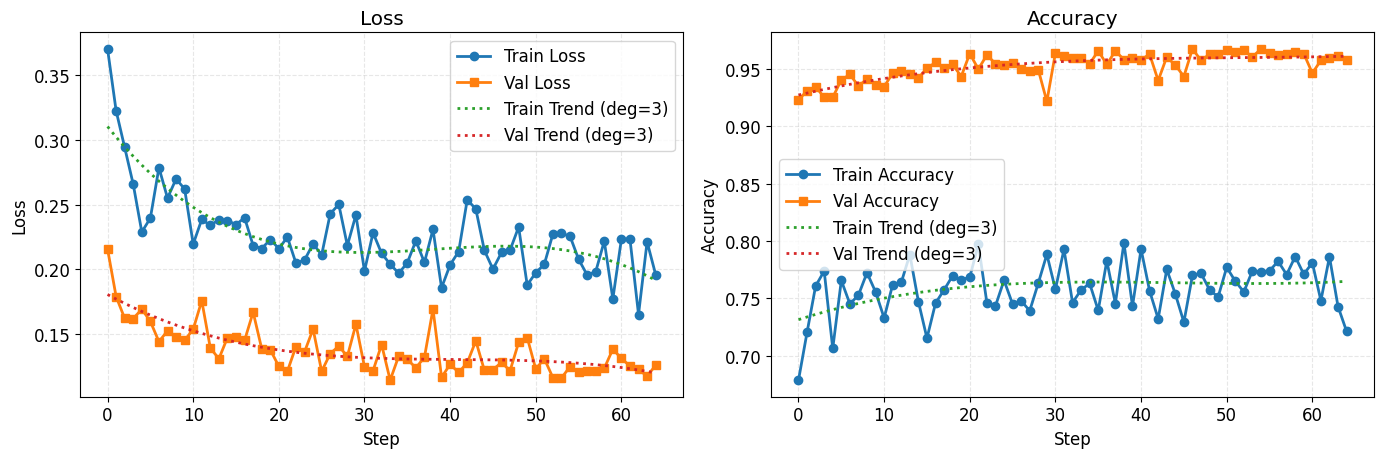
\includegraphics[width=\linewidth]{Bilder/jpg/conv_1d_train.png}
    \caption{Loss and Accuracy plots for training and validation for ConvNext V2 on dataset-1D}
    \label{conv_1d_train}
\end{figure}

Table~\ref{conv_1d_test} summarizes the ConvNext model's performance on the dataset-1D. The overall test loss of 0.36 and accuracy of 87.55\% indicate that the model generalizes well to held-out examples. From the confusion matrix (lower block of the table), we see that of 1591 true background samples the model correctly labels 1454 (91.4\% recall) and of 987 true walking events it correctly labels 803 (81.4\% recall). Precision scores 88.8\% for background and 85.4\% for walking confirming the model makes relatively few false alarms in each class.

\begin{table}[ht]
    \centering
    \caption{Test results for the ConvNext V2 model on the dataset-1D}
    \label{conv_1d_test}
    \begin{tabular}{lcc}
      \toprule
      \textbf{Metric}            & \textbf{Background} & \textbf{Walking} \\
      \midrule
      Test Loss                  & \multicolumn{2}{c}{0.3625}          \\
      Test Accuracy (\%)         & \multicolumn{2}{c}{87.55}           \\
      \addlinespace
      \multicolumn{3}{l}{\textbf{Confusion Matrix}} \\
      \quad True Background      & 1454                & 137             \\
      \quad True Walking         & 184                 & 803             \\
      \addlinespace
      \multicolumn{3}{l}{\textbf{Per-class Precision, Recall, F1 (\%)}} \\
      Precision                  & 88.77               & 85.43           \\
      Recall                     & 91.39               & 81.36           \\
      F1 Score                   & 90.06               & 83.34           \\
      \bottomrule
    \end{tabular}
  \end{table}
  
The graphs~\ref{eff_1d_train} show the loss and accuracy plots for training and validation of EfficientNet model on dataset-1D. Over 65 epochs, training is done. The train loss (blue) starts at 3.05 and gradually drops till it reaches 0.281. The validation loss (orange) starts at around 2 and gradually drops till it reaches 0.18. The minor spike is observed around 30th epoch but recover quickly. The train accuracy (blue) rises from 64\% to 75\% reflecting incremental learning. The validation accuracy (orange) starts at 72\% and rises till 90\% while plateauing between 88\% and 93\%. The learning summarizes good generalization.

\begin{figure}[h]
    \centering
    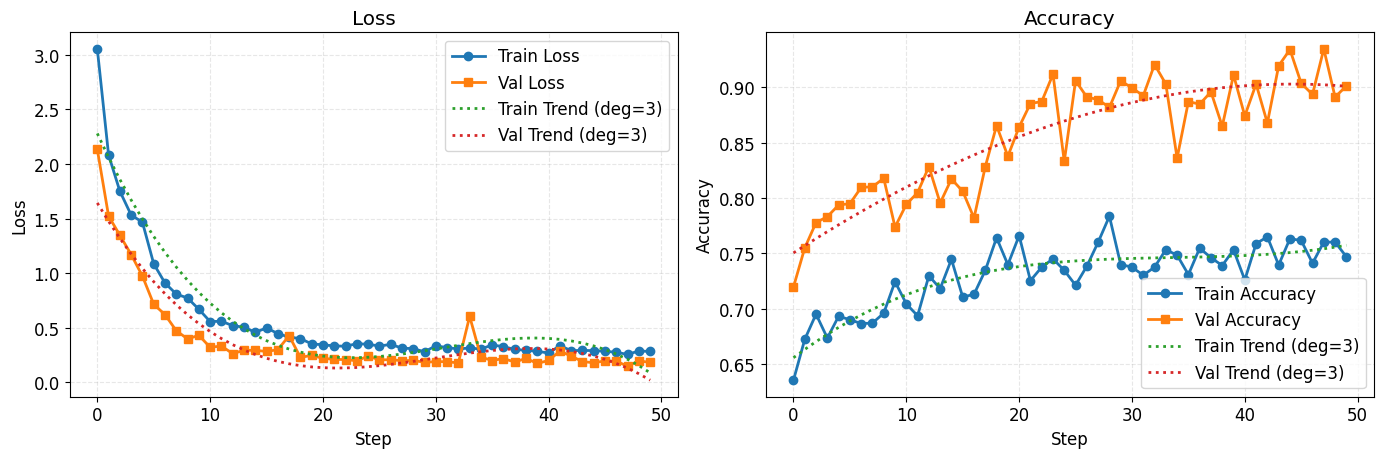
\includegraphics[width=\linewidth]{Bilder/jpg/eff_1d_train.png}
    \caption{Loss and Accuracy plots for training and validation for EfficientNet on dataset-1D}
    \label{eff_1d_train}
\end{figure}

\begin{table}[ht]
    \centering
    \caption{Test results for the EfficientNet model on dataset-1D}
    \label{eff_1d_test}
    \begin{tabular}{lcc}
      \toprule
      \textbf{Metric}            & \textbf{Background} & \textbf{Walking} \\
      \midrule
      Test Loss                  & \multicolumn{2}{c}{0.2496}          \\
      Test Accuracy (\%)         & \multicolumn{2}{c}{91.89}           \\
      \addlinespace
      \multicolumn{3}{l}{\textbf{Confusion Matrix}} \\
      \quad True Background      & 1512                & 79              \\
      \quad True Walking         & 130                 & 857             \\
      \addlinespace
      \multicolumn{3}{l}{\textbf{Per-class Precision, Recall, F1 (\%)}} \\
      Precision                  & 92.08               & 91.56           \\
      Recall                     & 95.03               & 86.83           \\
      F1 Score                   & 93.54               & 89.13           \\
      \bottomrule
    \end{tabular}
  \end{table}
  
Table \ref{eff_1d_test} reports the EfficientNet models performance on the dataset-1D. The model achieves a test loss of 0.25 and overall accuracy of 91.89\%, demonstrating strong generalization. Examining the confusion matrix, 95.0\% of true background samples (1512 out of 1591) are correctly identified, while 86.8\% of true walking events (857 out of 987) are detected. Precision remains high for both classes 92.1\% for background and 91.6\% for walking indicating few false alarms. Finally, F1 scores of 93.5\% and 89.1\% reflect a solid balance between precision and recall in each category.

The graph~\ref{conv_2d_train} shows the training and validation loss and accuracy plots of ConvNext V2 model on dataset-2D. The train loss (blue) and validation loss (orange) declines steeply where train loss drops from 0.56 to 0.20 at epoch 3 and validation loss plunges even faster from 0.88 to 0.06 at epoch 2. Train loss sees occasianl small upticks at epoch 5 but stablizes later. Validation loss remians low with tiny spikes at around epochs 11 and 21. Train accuracy (blue) starts around 57\% and reaches 85\% at epoch 10 then osscilates between 82\%-87\%. Validation accuracy (orange) skyrockets to 99\% at epoch 3 and stay high with some minor dips at around at epoch 11 and 21 suggesting good learning. 

\begin{figure}[h]
    \centering
    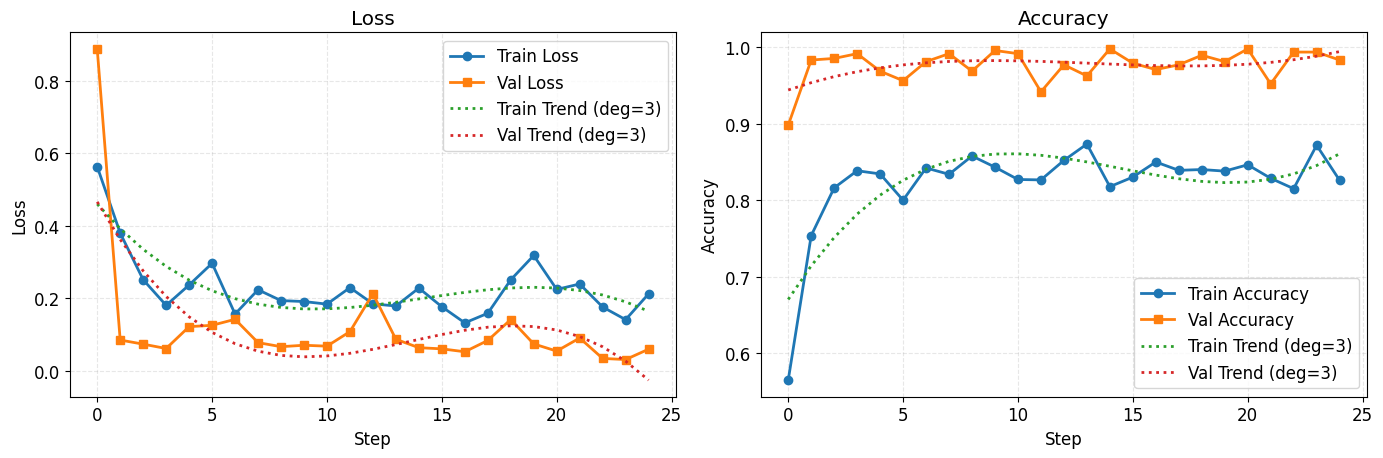
\includegraphics[width=\linewidth]{Bilder/jpg/conv_2d_train.png}
    \caption{Loss and Accuracy plots for training and validation for ConvNext V2 with 10 spatial channels and 2 sample length}
    \label{conv_2d_train}
\end{figure}

\begin{table}[ht]
    \centering
    \caption{Test results for the ConvNeXt V2 model on the dataset-2D}
    \label{conv_2d_test}
    \begin{tabular}{lcc}
      \toprule
      \textbf{Metric}            & \textbf{Background} & \textbf{Walking} \\
      \midrule
      Test Loss                  & \multicolumn{2}{c}{0.0537}          \\
      Test Accuracy (\%)         & \multicolumn{2}{c}{99.48}           \\
      \addlinespace
      \multicolumn{3}{l}{\textbf{Confusion Matrix}} \\
      \quad True Background      & 1678                & 4               \\
      \quad True Walking         & 5                   & 58              \\
      \addlinespace
      \multicolumn{3}{l}{\textbf{Per-class Precision, Recall, F1 (\%)}} \\
      Precision                  & 99.70               & 93.55           \\
      Recall                     & 99.76               & 92.06           \\
      F1 Score                   & 99.73               & 92.80           \\
      \bottomrule
    \end{tabular}
  \end{table}

Table~\ref{eff_2d_test} presents the ConvNext V2 model's performance on the dataset-2D. The extremely low test loss of 0.0537 and very high overall accuracy of 99.48\% show that the model almost perfectly separates footsteps from background. In the confusion matrix, 1678 out of 1682 background samples are correctly classified (99.8\% recall), and 58 out of 63 walking events are detected (92.1\% recall). Precision remains excellent 99.7\% for background and 93.6\% for walking indicating virtually no false alarms in the background class and very few in the walking class. The resulting F1 scores (99.7\% for background, 92.8\% for walking) confirm a close to ideal balance of precision and recall.

The graph~\ref{eff_2d_train} shows the train loss and accuracy set for ConvNeXt V2 on dataset-2D. The model runs over 25  epochs. The train loss (blue) and validation loss (orange) have a rapid intial drops over first 3-4 epochs indicating model picks up on low-level features. After that decline is more gradual and settles at 0.2 to 0.3. The sharp spike at epochs 11-12 suggesting model destabilzes then model recovers. Train accuracy (blue) rises from 63\% to 80\% and pleateauing at the point. Validation accuracy (orange) jumps from 66\% to 91\% which dips at epoch 4 to 58\% then agian recovers. The graph demonstarates the good genralization over the data.

\begin{figure}[h]
    \centering
    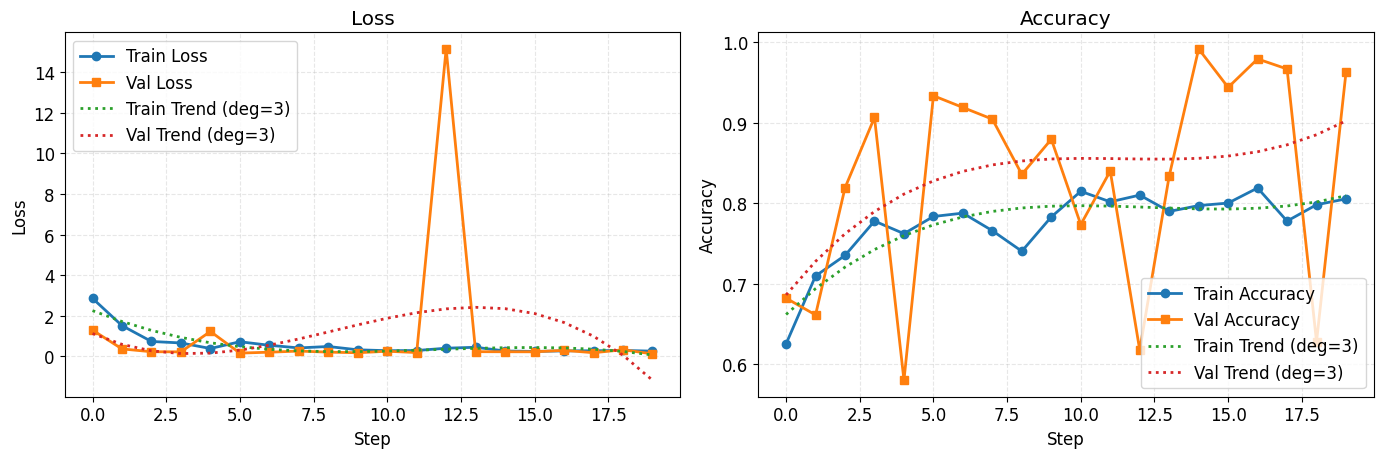
\includegraphics[width=\linewidth]{Bilder/jpg/eff_2d_train.png}
    \caption{Loss and Accuracy plots for training and validation for EfficientNet with 10 spatial channels and 2 sample length}
    \label{eff_2d_train}
\end{figure}

\begin{table}[ht]
    \centering
    \caption{Test results for the EfficientNet model on the 2-D dataset}
    \label{eff_2d_test}
    \begin{tabular}{lcc}
      \toprule
      \textbf{Metric}            & \textbf{Background} & \textbf{Walking} \\
      \midrule
      Test Loss                  & \multicolumn{2}{c}{0.0934}          \\
      Test Accuracy (\%)         & \multicolumn{2}{c}{99.48}           \\
      \addlinespace
      \multicolumn{3}{l}{\textbf{Confusion Matrix}} \\
      \quad True Background      & 1679                & 3               \\
      \quad True Walking         & 6                   & 57              \\
      \addlinespace
      \multicolumn{3}{l}{\textbf{Per-class Precision, Recall, F1 (\%)}} \\
      Precision                  & 99.64               & 95.00           \\
      Recall                     & 99.82               & 90.48           \\
      F1 Score                   & 99.73               & 92.68           \\
      \bottomrule
    \end{tabular}
  \end{table}

Table~\ref{eff_2d_test} summarizes the EfficientNet model's performance on dataset-2D With a test loss of only 0.934 and an overall accuracy of 99.48\%, the network distinguishes footsteps from background almost flawlessly. The confusion matrix shows that 1679 out of 1682 background samples are correctly identified (99.8\% recall), while 57 out of 63 walking events are detected (90.5\% recall). High precision values 99.6\% for background and 95.0\% for walking indicate very few false positives. Finally, F1 scores of 99.7\% and 92.7\% confirm an excellent balance between precision and recall for each class.

The metrics in the graphs suggests that models shows the similar performance over the testing set for the same models training set. Except the ConvNext V2 model on dataset-1D, all the other show similar performance and are better than ConvNext V2 model on dataset-1D. The checkpoints should be evaluated on real-time across the data stream coming in through the DAS configurator application. Model should show similar performance as the performance on testing set. 

\section{Real-time evaluation Framework}
\label{sec:realtime_evaluation}
For real time evaluation of the model, the data needs to be streamed to the model and based on the data the model is able to classify the data. This is done with the help of \texttt{spectrogram\_classifier} module which is used for the real-time evaluation and developed with the help of \texttt{dasdpu} package. The \texttt{dasdpu} package is an internal package developed at AP Sensing for running and testing algorithms on DAS DPU or locally on HDF5 files. It is used for socket reading of Frequency Band Energy (FBE) and/or phases data. It also sends the events or alarms to the DPU such that are displayed in the Configurator. This package is one of the most important elements in the real-time evaluation script.

Spectrogram Classifier (\texttt{spectrogram\_classifier}) is the module developed internally at AP Sensing which is used for evaluation of the models. The module implements the online execution of the logic for the phase-based footstep detection. It ingests the raw phase samples from the DAS-acquisition service, buffers a short user-defined time window, and optionally computes the spectrograms for each channel before forwarding them to the trained model. When the model's output probability exceeds the user-set threshold, the pipeline emits a detection. The detections are tracked over time by grouping and assigning them track IDs, thus allowing the tracking of a moving disturbance along the cable. Once a track accumulates sufficient repeated detections (confidence), the alarm is raised. Figure~\ref{dg_spectrogram} gives an overview of the structure of the \texttt{spectrogram\_classifier} module and it's dependencies to all other packages. All the standard python libraries on which the module is dependant on are excluded. The dependencies with \texttt{dasdpu} and other packages is shown in the figure~\ref{dg_spectrogram}. The \texttt{system.py} is the file which which has all the logic files essential for the working of the module and is the file where all the changed files are imported. 

\begin{figure}[h]
    \centering
    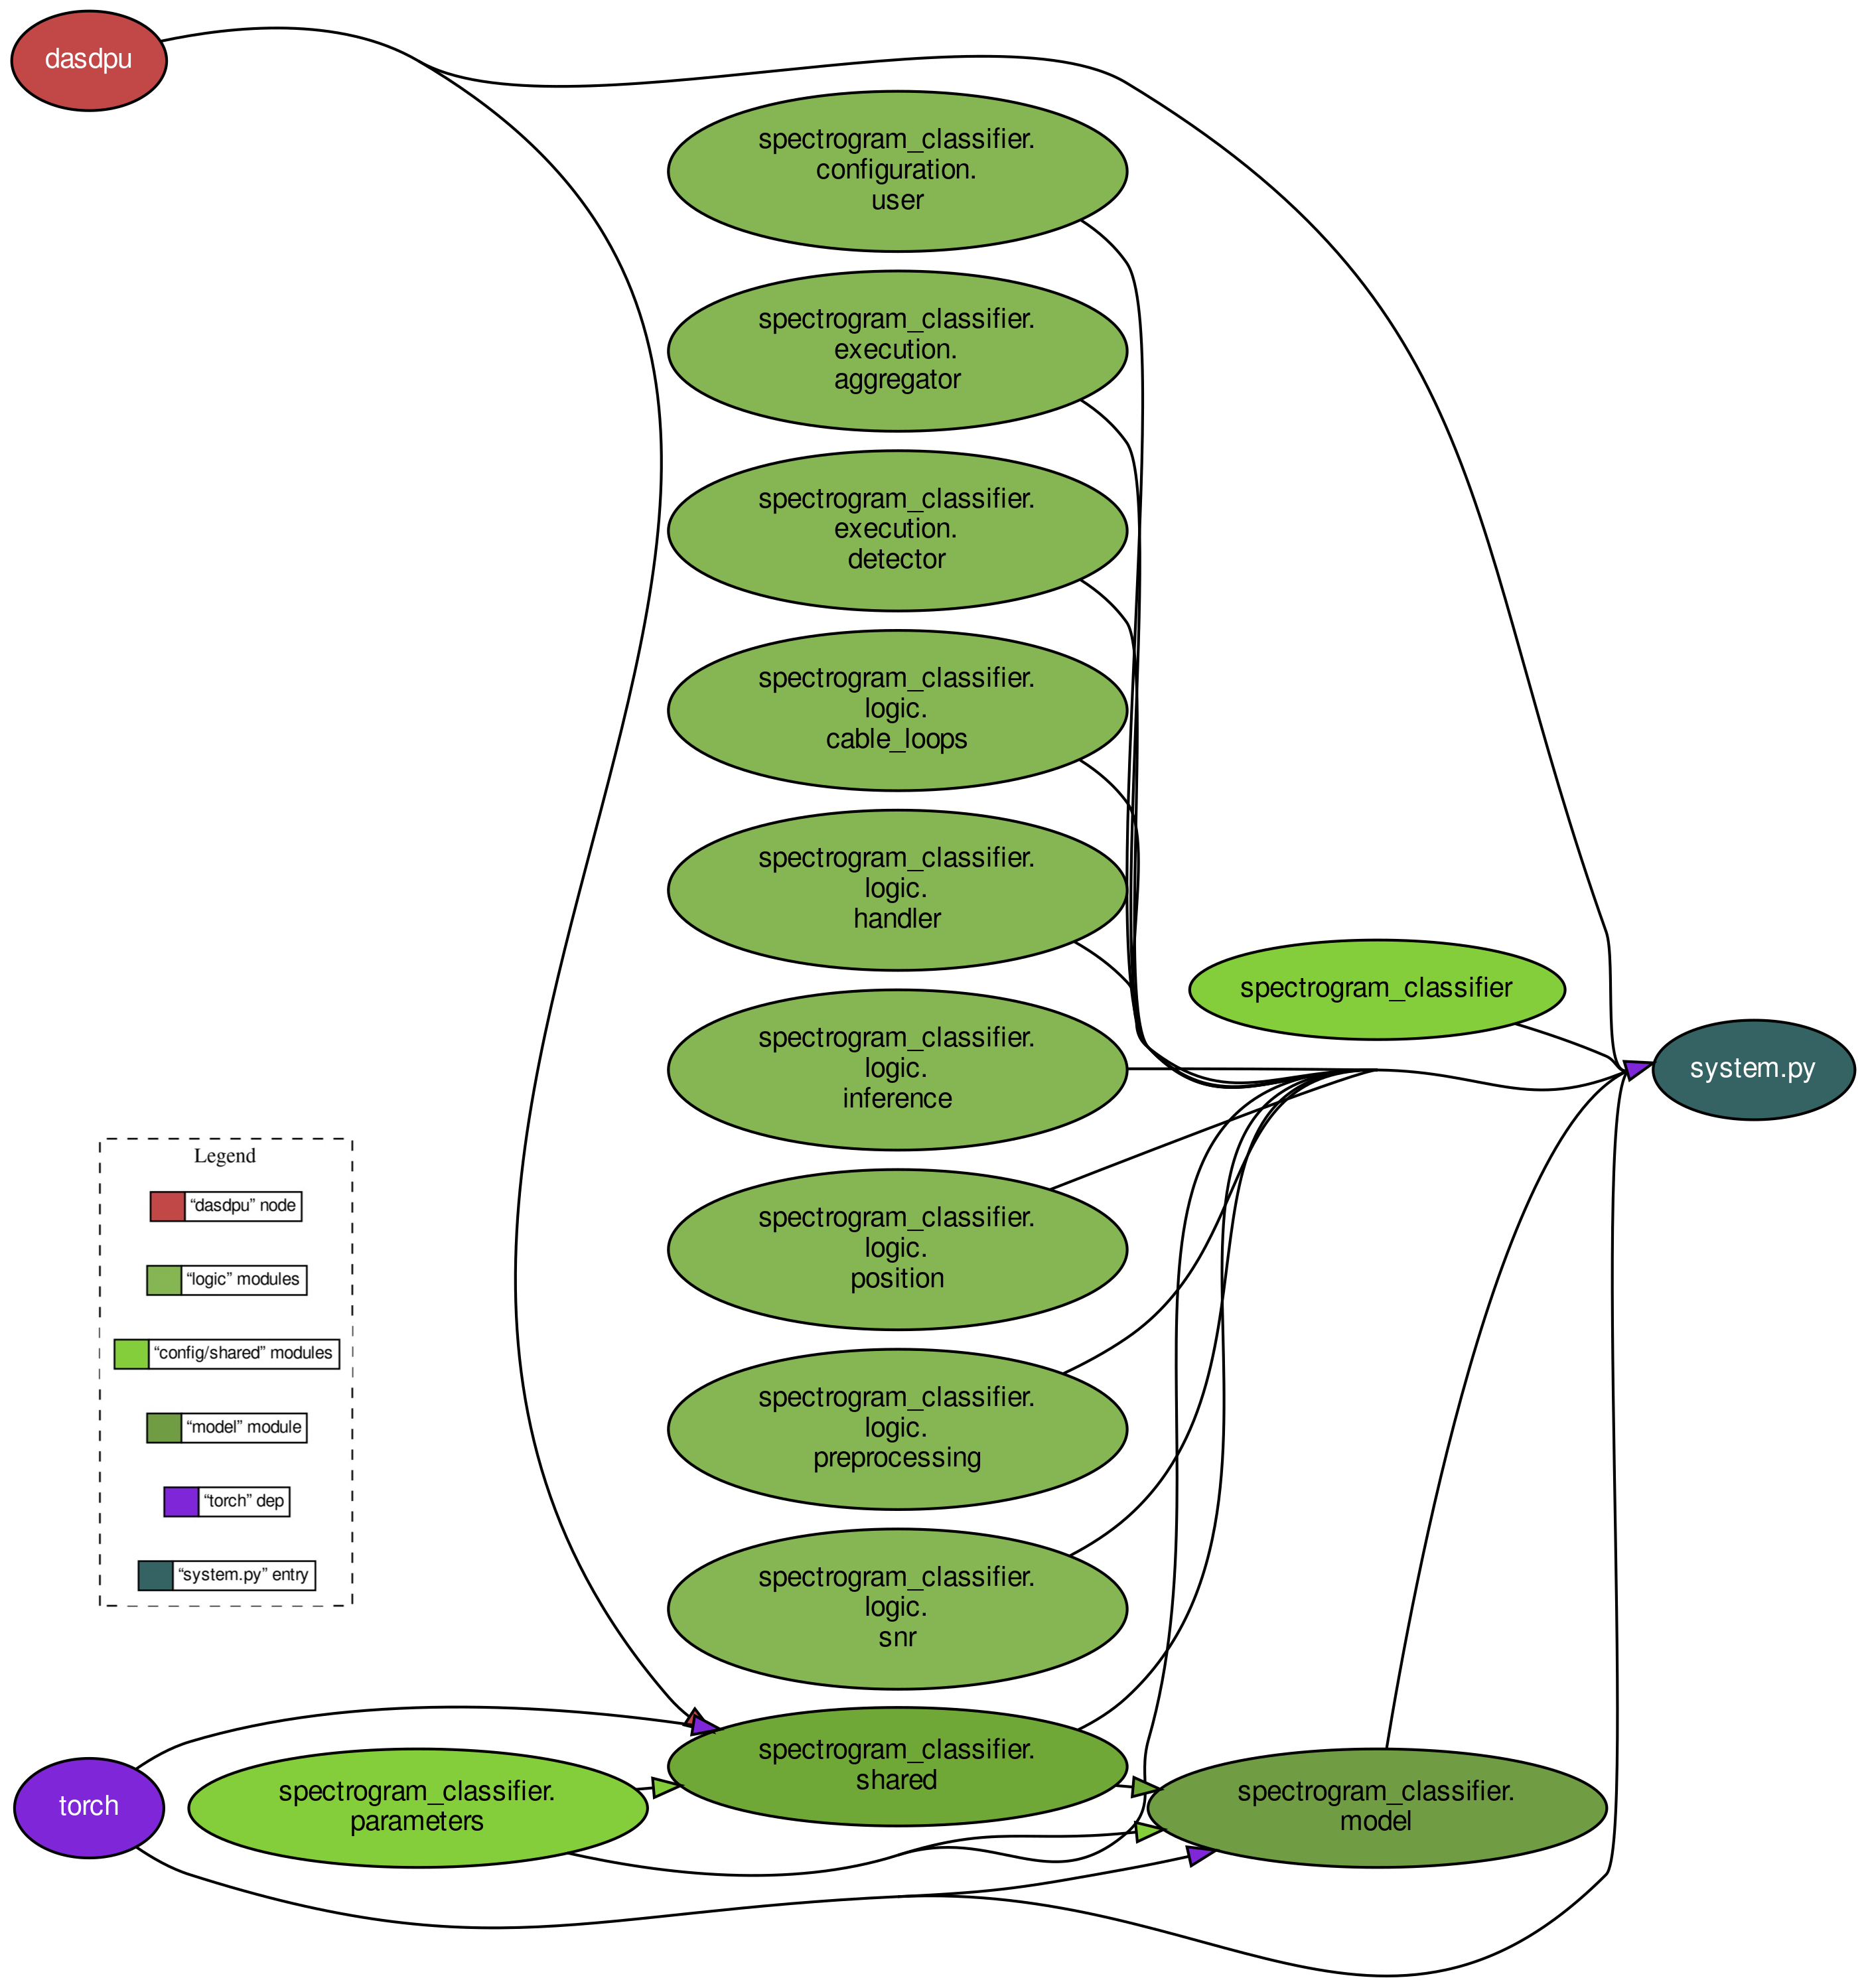
\includegraphics[width=\linewidth]{Bilder/jpg/output_graph.png}
    \caption{Dependency Graph of \texttt{spectrogram\_classifier} module}
    \label{dg_spectrogram}
\end{figure}

The \texttt{spectrogram\_classifier.execution.aggregator} and \texttt{spectrogram\_classifier.execution.detector} are the top level files responsible for the execution. The \texttt{spectrogram\_classifier.logic.inference} returns the list of detections from the tensor. Position in terms of distance is mapped from \texttt{spectrogram\_classifier.logic.position} from the spatial channels. All the remaining files are not crucial for detection but serve as the support and enables in smooth running of the system. The \texttt{spectrogram\_classifier} module is edited to adjust for the preprocessing steps done while training the model and models ConvNext V2 and EfficientNet are also added in the pipeline for easy selection and switching. The preprocessing section is inserted in the \texttt{spectrogram\_classifier.logic.preprocessing} which is same as the training. The model is inserted in the \texttt{spectrogram\_classifier.model} is also same as the training.

\begin{lstlisting}[style=pythonstyle, caption={Preprocessing for conversion of raw phase data to spectrogram in the framework}, label=lst:stft_processing]
class SpectrogramPreprocessorStft:
    def __init__(self, model_params: Parameters, data_rate_hz: int = 1000, device: torch.device = torch.device("cuda")):
        self._data_rate_hz = data_rate_hz
        self._device = device
        self._multiplier = data_rate_hz // 500
        self._nperseg = 128 * self._multiplier
        self._noverlap = self._nperseg - 14 * self._multiplier
        self._f_bank = (
            melscale_fbanks(
                n_freqs=self._nperseg // 2 + 1,
                f_min=model_params.f_min,
                f_max=model_params.f_max,
                n_mels=model_params.n_mels,
                sample_rate=data_rate_hz,
                mel_scale="htk",
                norm=None,
            )
            .cpu()
            .numpy()
        )

    def preprocess(self, data: np.ndarray, axis: int) -> tuple[np.ndarray, np.ndarray]:
        data_accum = self._accum(data, axis=axis)
        f, t, stft = signal.stft(
            data_accum,
            fs=self._data_rate_hz,
            nperseg=self._nperseg,
            noverlap=self._noverlap,
            padded=False,
            scaling="psd",
            axis=axis,
        )
        stft = np.abs(stft) ** 2
        stft = np.matmul(stft.transpose((0, 2, 1)), self._f_bank).transpose((0, 2, 1))
        mag = 10 * np.log10(stft)
        return 

    def process(self, tensor_data: torch.Tensor) -> torch.Tensor:  
        tensor_numpy = tensor_data.cpu().numpy()
        numpy_result = self.data_process(tensor_numpy, axis=-1)
        return torch.from_numpy(numpy_result).float().cuda()  

    def _accum(self, x: np.ndarray, axis: int) -> np.ndarray:
        x = np.cumsum(x, axis=axis, dtype=np.int64).astype(np.float32) * INT_TO_RADIANS
        sos = signal.butter(2, 5, "hp", fs=1000, output="sos")
        x = signal.sosfiltfilt(sos, x, axis=axis)
        return x

    @property
    def device(self) -> torch.device:
        return self._device

\end{lstlisting}

The listing~\ref{lst:stft_processing} shows the processing which is same as the listing in the section listing~\ref{lst:mag_processing}. The main difference is that data is in the form a tensor in listing~\ref{lst:stft_processing} so it first needs to be converted into a numpy for the STFT function which is used in preprocessing in training pipeline. After the STFT function in \texttt{preprocess} the shape needs to be considered as the streamed data for realtime since it needs to be in the format \texttt{[batch, frequency\_bins, time]} in comparison to training where the shape is adjusted after extracting the data in listing~\ref{lst:binfile_dataset}. The \texttt{\_accum} function has the cumulative sum where it is done on the time axis as the data distorts and the model will not be able to do the detections.

\begin{lstlisting}[style=pythonstyle, caption={Model evaluation mode in the framework}, label=lst:model_rt]
def get_effnet_b0(params: Parameters) -> torch.nn.Module:
    return timm.create_model("efficientnet_b0", num_classes=params.n_classes, in_chans=params.model_n_channels)

def get_convnextv2(params: Parameters) -> torch.nn.Module:
    return timm.create_model("convnextv2_atto", num_classes=params.n_classes, in_chans=params.model_n_channels)

def create(cls, weights_path: str | Path, device=torch.device("cpu")) -> Model:

    model_data = torch.load(weights_path)
    state_dict = model_data["model_state_dict"]
    mean = model_data["mean"]
    std = model_data["std"]

    params = Parameters(
        epochs=100,
        batch_size=32,
        test_batch_size=32,
        learning_rate=1e-3,
        weight_decay=1e-4,
        dataset_mean=mean.reshape((1, 1, 1, 1)),
        dataset_std=std.reshape((1, 1, 1, 1)),
        label_smoothing=0.1,
        accum_phase=False,
        highpass_cutoff_hz=None,
        expected_data_rate_hz=1000,
        n_fft=512,
        hop_size=256,
        pad=0,
        center=True,
        mel_scale=False,
        n_mels=64,
        f_min=0,
        f_max=500,
        model_name="effnet-b0",
        model_d=64,
        n_classes=2,
        model_n_channels=10,
        normalization="global",
    )

    model = create_model(params, state_dict)
    model = TimmModelWrapper(model, mean=mean, std=std)
    model = model.eval()

    return cls(model, device, params)

\end{lstlisting}

The listing~\ref{lst:model_rt} shows the evaluation mode for ConvNext V2 and EfficientNet. These functions are used in the top layer of the model where the parameters like classes and input channels are given to the functions from parameters that are used. The  parameters used in the model are set to the same values which are used while training. The mean and standard deviation calculated during the training ans stored in the checkpoint are extracted and used for normalization of data. The model is created using \texttt{create\_model} function which calls either \texttt{get\_convnextv2} or \texttt{get\_effnet\_b0} based on the model name. The model is wrapped in \texttt{TimmModelWrapper} which is used to adjust the shape and set the normalization parameters. The model is then set to evaluation mode for returning detections

% ===============================
% ===============================
%  Kapitel 5 - Test und Messungen
% ===============================
% ===============================

\chapter{Evaluation}
\label{ch:evaluation}

In this chapter, assessment of trained models is done on truly unseen data-recordings captured via the DAS configurator but never used during training or validation. The steps such as employing a real-time processing script that streams raw phase data, applies the same preprocessing pipeline, and loads the saved model checkpoints for footstep detection. The evaluation is done using the \texttt{spectrogram\_classifier} framework which is explained in the section~\ref{sec:realtime_evaluation}. Finally, comparison of the performance of different architectures and concise analysis of their relative strengths and weaknesses will be given.

\section{Real-time Evaluation of the  Model}

Evaluation of the model is performed by loading the data recordings from the DAS configurator application and streaming the data to the model using the \texttt{spectrogram\_classifier} framework. Framework is designed to handle live data streams and give out the detection on the DAS configurator application. Evaluation also needs the checkpoint files of the trained models. Sample length(seconds) and number of spatial channels need to be configured based on the checkpoint files used as the model is trained on two different types of dataset. 

Listing~\ref{lst:config_yaml} shows the \texttt{YAML} configuration file~\cite{pyyaml} for the real-time evaluation framework. The \texttt{window\_len\_secs} and \texttt{hop\_len\_secs} parameters together define the duration of each analysis frame and the time shift between successive frames, respectively, controlling how the continuous DAS stream is chopped into overlapping segments for spectrogram generation. In the activities section identifiers are assigned used by the DAS Configurator to label detections, while the \texttt{zones} section defines spatial intervals via \texttt{start\_m} and \texttt{end\_m} within which the classifier is active. Finally, \texttt{min\_prob} sets the minimum confidence threshold for an event to be reported, filtering out low-probability (and likely false-positive) detections. Careful tuning of these settings is key to achieving efficient, reliable performance.

The \texttt{device} parameter specifies where the model is loaded (e.g., \texttt{cuda} or \texttt{cpu}), and \texttt{dtype} sets the tensor data type used throughout processing. Incoming DAS data are buffered for up to \texttt{max\_age\_sec} seconds, and once the model reports at least \texttt{min\_confidence} detections within that window, an alarm is issued. To control memory use, the framework processes data in fixed-size blocks of channels, as defined by \texttt{n\_channels\_per\_block}, which should match the host's available RAM or GPU capacity. Enabling \texttt{save\_debug\_data} will write every raw detection to \texttt{.npy} files for offline inspection. 
Each channel is classified as either walking or background. Consecutive "walking" samples that span at least \texttt{min\_size\_m} meters trigger an event, and if that event continues into the next time step within \texttt{max\_distance\_m} meters, it is merged and its confidence count increments. Since we do not apply any SNR-based filtering, \texttt{min\_snr} is fixed to zero. Finally, \texttt{tensor\_idx} selects which output index corresponds to each class (e.g.\ 1 for walking, 0 for background). All of these parameters remain fixed during evaluation to ensure a consistent runtime behavior.

\begin{lstlisting}[style=pythonstyle, caption={YAML configuration for the real-time DAS evaluation framework}, label={lst:config_yaml}]
window_len_secs: 2
hop_len_secs: 1
device: cuda
dtype: float16
n_channels_per_block: 500
save_debug_data: true
activities:
  person_walking:
    max_age_sec: 10
    min_confidence: 4
    min_size_m: 0
    max_distance_m: 15
    min_snr: 0
    tensor_idx: 1
    zones:
      - start_m: none
        end_m: none
        min_prob: 0.92
\end{lstlisting}

For our evaluation, we recorded a straight-line footstep trail of approximately one minute's continuous walking about 45 individual steps performed by a different person than those in the training set to test across subject generalization. The walker maintained a steady pace without turns or pauses along the same fiber route used for training, isolating pure step-to-step detection performance. Because our models were trained on very short clips (2-5 footsteps), evaluating them on this longer sequence stresses the pipeline's temporal grouping logic. All detections and alarms were logged within a 75 m zone of interest and then compared against the known ground-truth step positions to measure both spatial and temporal accuracy. We also verified the pipeline under both slower and faster gait speeds and observed very similar spatial temporal detection patterns; accordingly, our detailed results focus on the steady-pace walking described above.

\subsection{ConvNext V2 Model evaluation}
\label{sec:conv_eval}
The ConvNext V2 model is trained on two different datasets - Dataset-1D and Dataset-2D as explained in section~\ref{sec:dataset}. There are two checkpoints for ConvNext V2 model for both datasets. Using these checkpoints the evaluation is done for over the data collected. 
\begin{figure}[h]
  \centering
  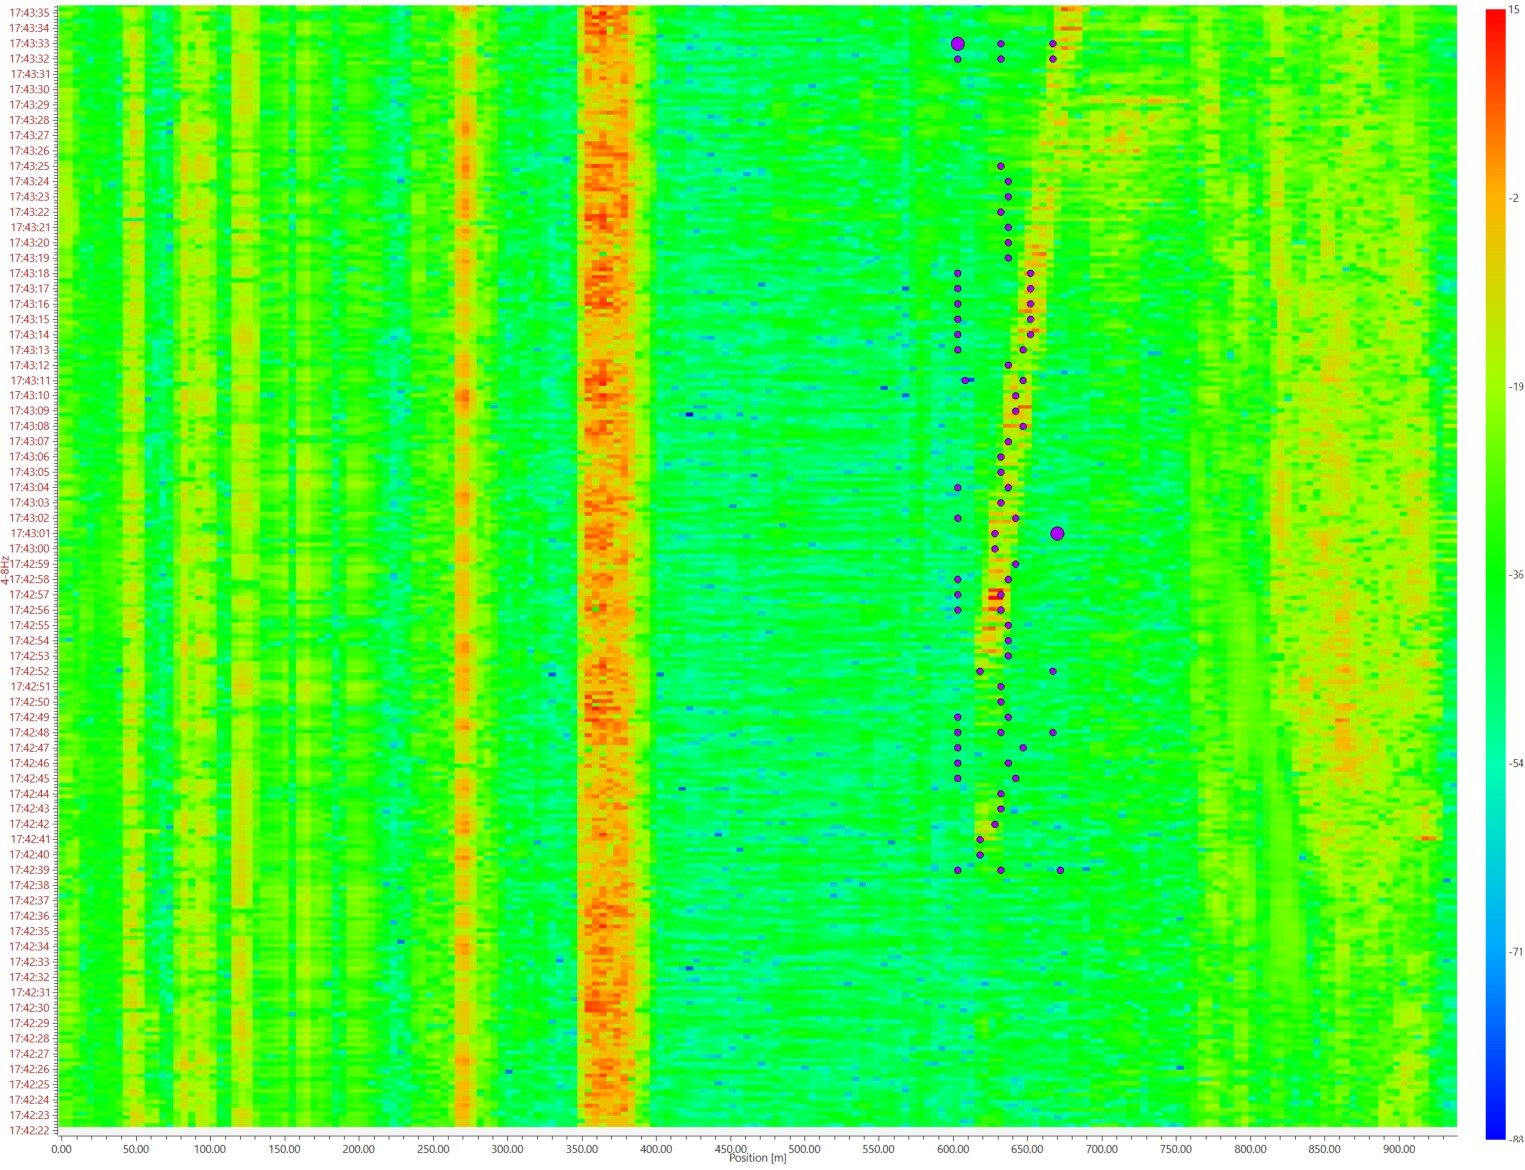
\includegraphics[width=0.9\linewidth]{Bilder/jpg/conv_1d_eval.jpg}
  \caption{DAS Configurator Application detections for ConvNext V2 model on dataset-1D}
  \label{conv_1d_eval}
\end{figure}

The checkpoint file for dataset-1D is loaded into the framework for evaluation. The \texttt{window\_len\_secs} is set to 1.728 seconds and \texttt{hop\_len\_secs} is set to 1 second. Zone is set between 600 to 675 meters to focus on the area as too many detections are generated if the entire files given and application is not able to handle them. Threshold is set to 0.9 to remove the false positives. Figure~\ref{conv_1d_eval} shows the detections after running the evaluation framework on the dataset-1D. 

The detections are shown with the help of purple bubbles. The smaller bubbles are events and bigger bubbles are alarms. As seen in the figure~\ref{conv_1d_eval} there are around 70 detections which shows model is able to detect footsteps but also on the neighboring spatial channels. This shows detections is not perfect as the detections does not align with the footsteps and exact position cannot be determined.

\begin{figure}[h]
  \centering
  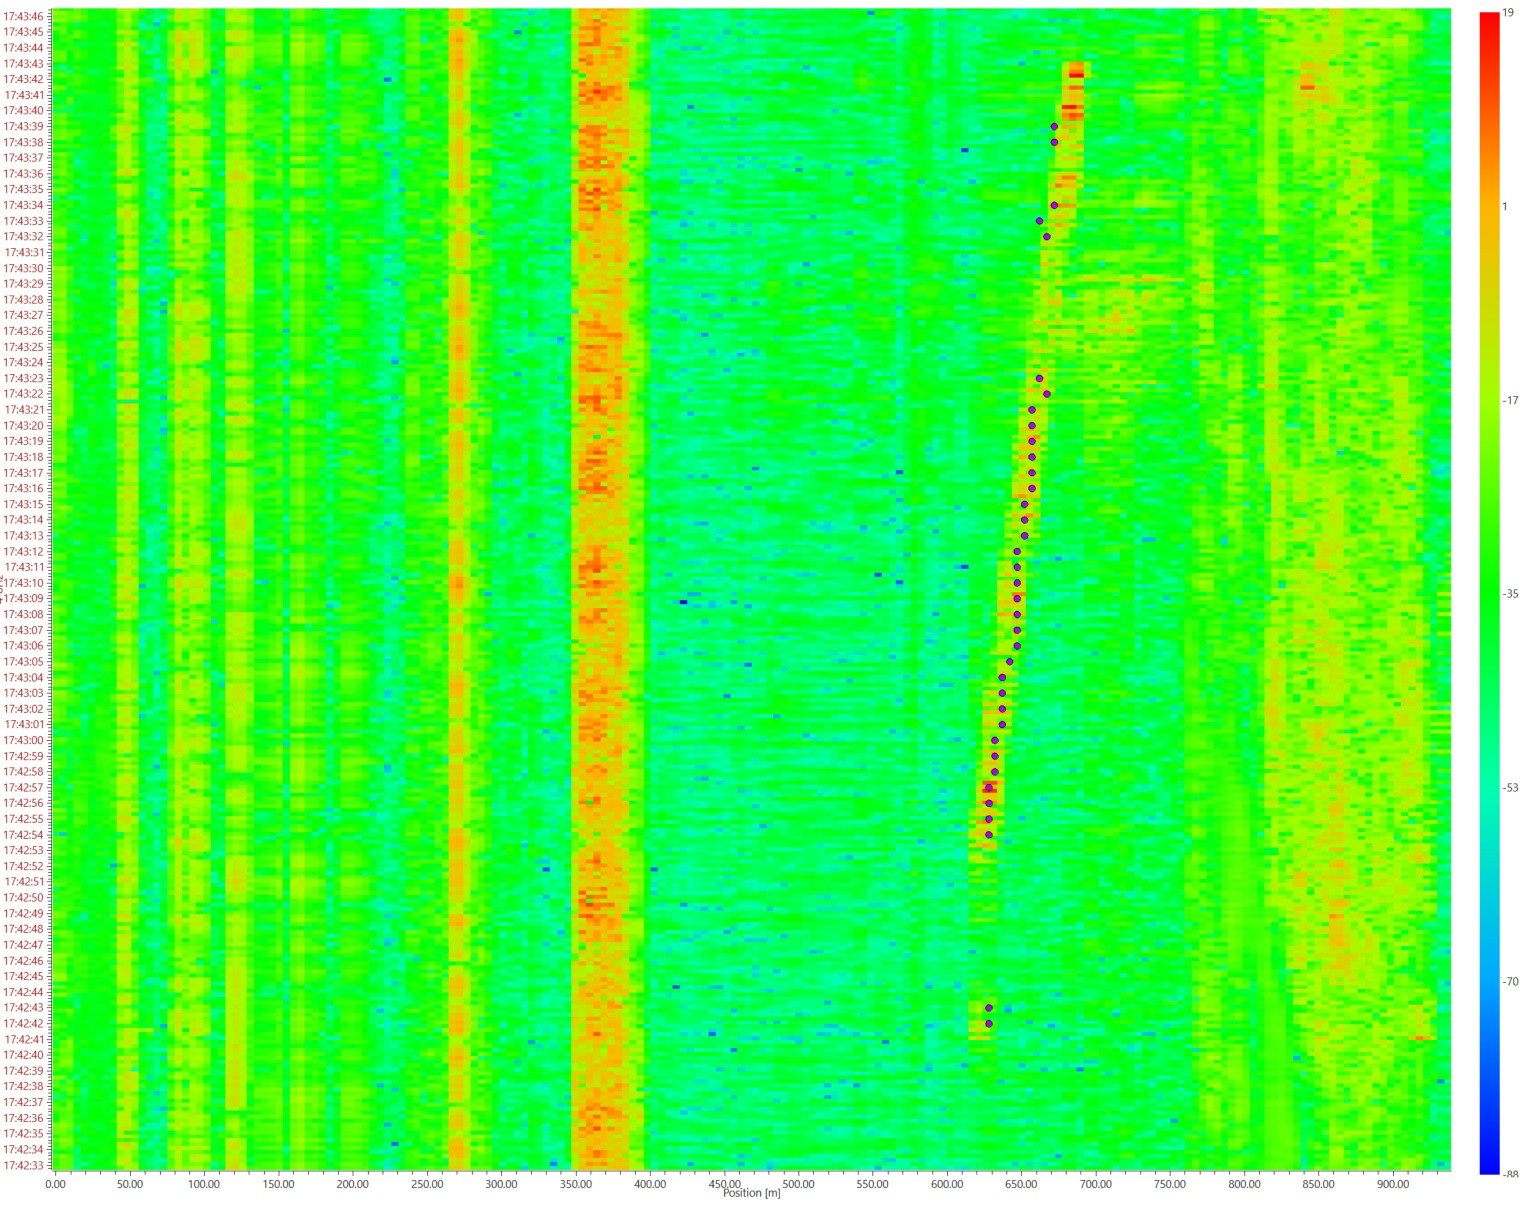
\includegraphics[width=0.9\linewidth]{Bilder/jpg/conv_2d_eval.jpg}
  \caption{DAS Configurator Application detections for ConvNext V2 model on dataset-2D}
  \label{conv_2d_eval}
\end{figure}

Now the checkpoint file for dataset-2D is loaded into the framework for evaluation. The \texttt{window\_len\_secs} and \texttt{hop\_len\_secs} are set to 2 seconds and 1 seconds respectively. Rest of the other parameters are kept the same. Figure~\ref{conv_2d_eval} shows the around 35 detections when evaluation framework is ran. The major difference from dataset-1D is that the footstep trail is more clear and there are lot less false positives with detections more aligned to the actual footstep trail.

From the accuracies over the respective datasets in section~\ref{sec:comp} it was evident that the model with dataset-2D is better than the dataset-1D as the accuracies were 87\% and 99\% respectively. The false positives are much lesser and the footsteps are more accurate in dataset-2D. 

\subsection{EfficientNet Model evaluation}
\label{sec:eff_eval}
EfficientNet Model is also trained in a similar fashion as ConvNext V2 model with dataset-1D and dataset-2D. Models with their respective checkpoints are evaluated by keep The EfficientNet model is selected in the framework in listing~\ref{lst:model_rt} and the number channels are also set according to the checkpoint file. 

\begin{figure}[h]
  \centering
  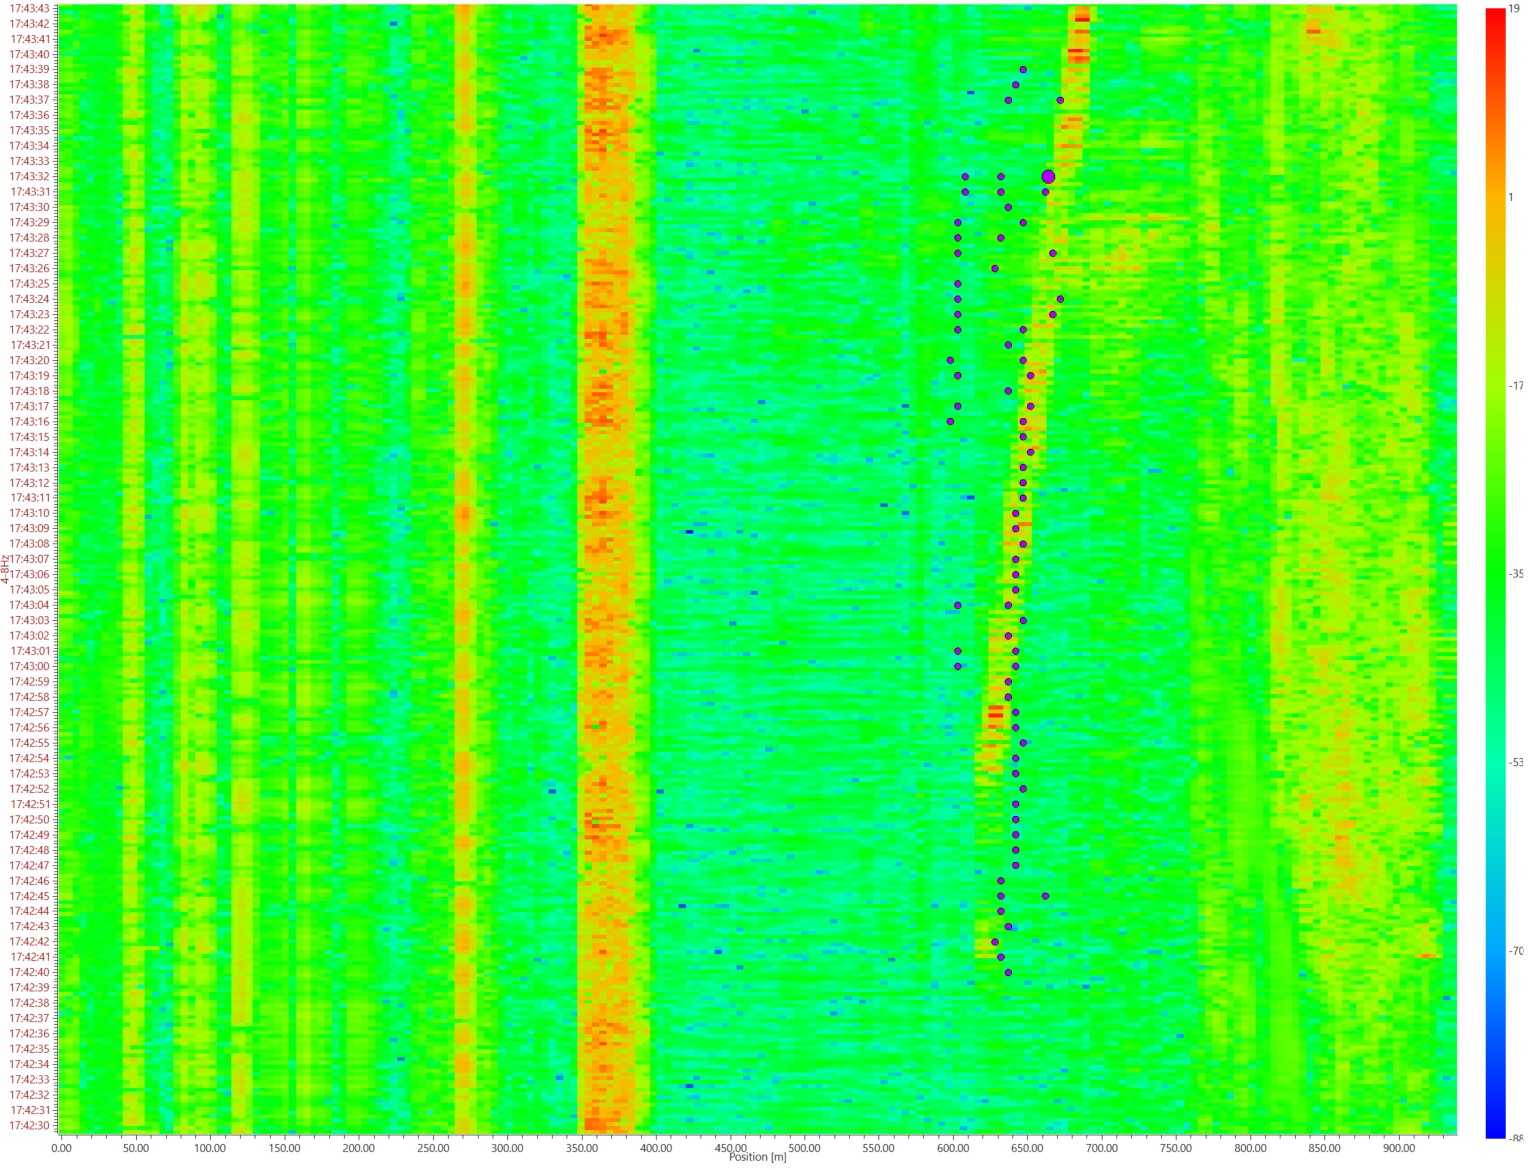
\includegraphics[width=0.9\linewidth]{Bilder/jpg/eff_1d_eval.jpg}
  \caption{DAS Configurator Application detections for EfficientNet V2 model on dataset-1D}
  \label{eff_1d_eval}
\end{figure}

The checkpoint file for dataset-1D is loaded into the framework nad the parameters are setup. The \texttt{window\_len\_secs} is set to 1.728 seconds and \texttt{hop\_len\_secs} is set to 1 second. Zone is selected the same as ConvNext V2 model which is between 600 to 675 meters to focus on a specific region. Threshold value is also kept same to 0.9 to make sure that only the detections with utmost certainty are recorded. 

Figure~\ref{eff_1d_eval} shows the about 70 detections by the model on dataset-1D. Detections are shown with purple bubbles with smaller ones as the events and bigger ones as alarms. The detections are similar to the ConvNext V2 model for dataset-1D. In a similar fashion, the model is able to detect the trail but with it there are lot of false positives on neighboring spatial channel. The exact position of footsteps is not determinable.  

\begin{figure}[h]
  \centering
  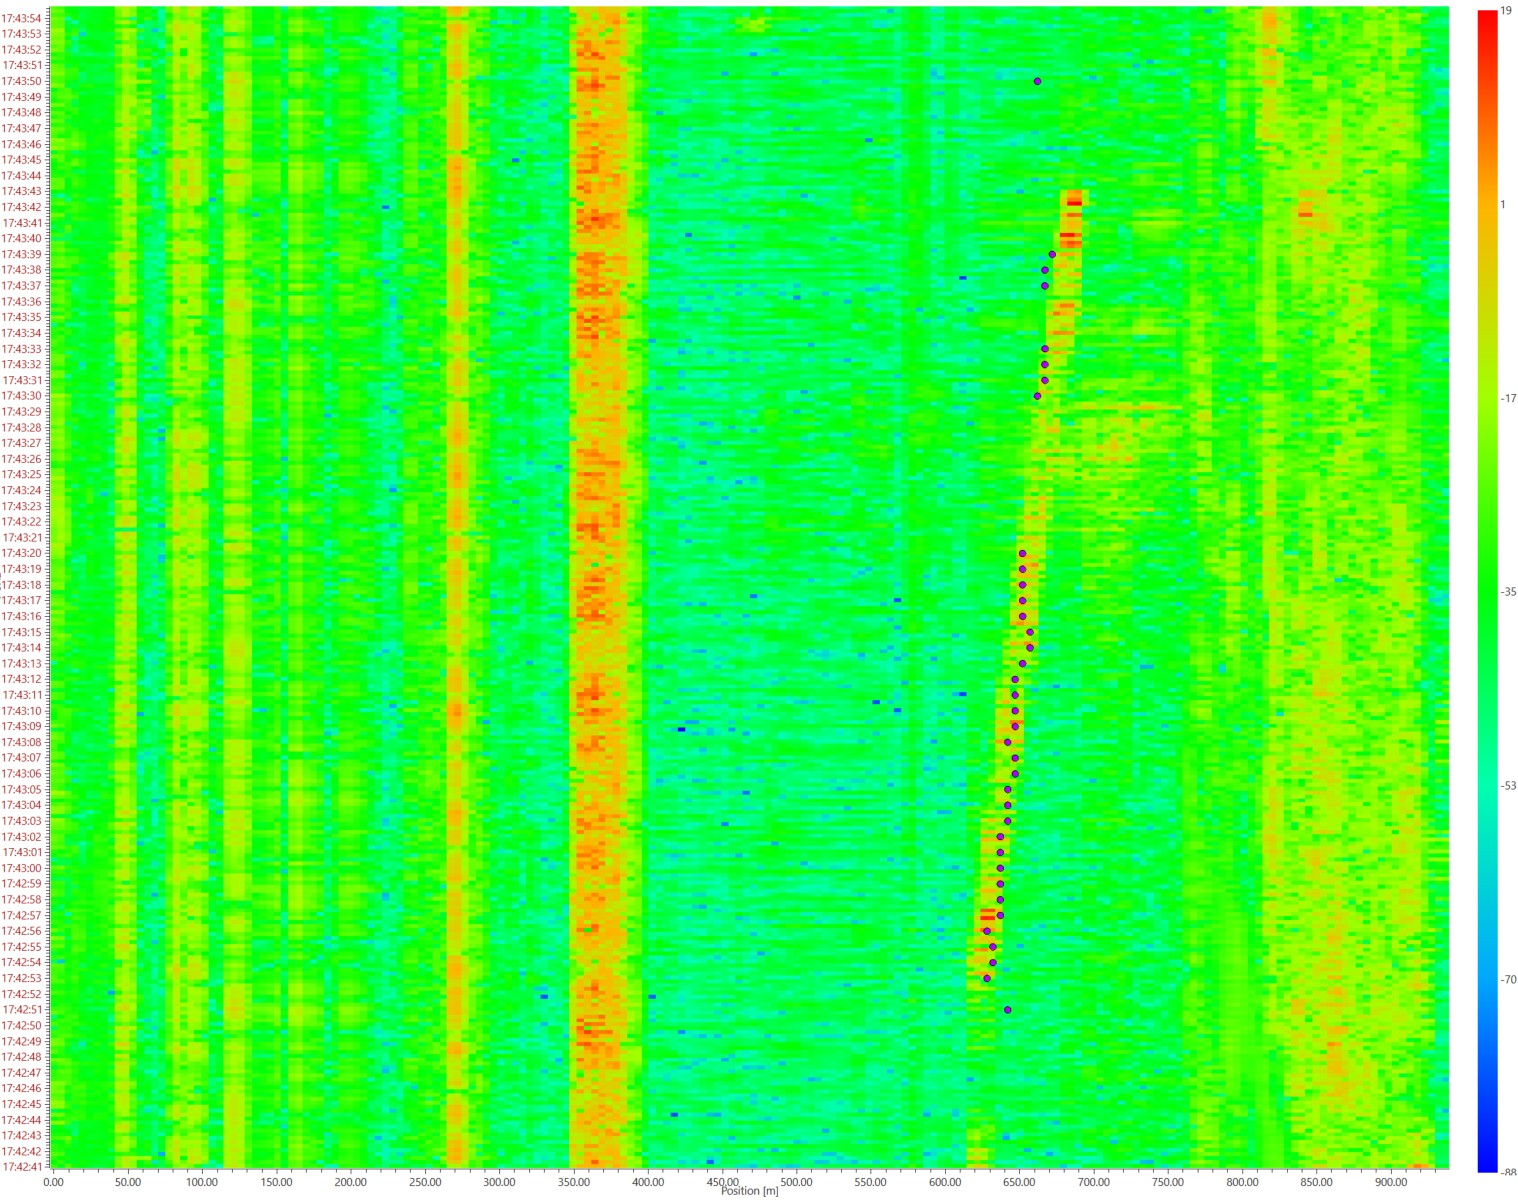
\includegraphics[width=0.9\linewidth]{Bilder/jpg/eff_2d_eval.jpg}
  \caption{DAS Configurator Application detections for EfficientNet V2 model on dataset-2D}
  \label{eff_2d_eval}
\end{figure}

Dataset-2D checkpoint file is loaded into the framework and parameters remain the same. Spatial channels are set to 10. The \texttt{window\_len\_secs} is et to 2 seconds and  \texttt{hop\_len\_secs} is et to 1 seconds. Zone is kept the same to focus on 600 to 675 meters. Threshold is also kept same at 0.9. Figure~\ref{eff_2d_eval} shows about 35 detections made when the evaluation framework is ran. The detections are much more accurate and focused on the footstep trail. Model performs similarly to the ConvNext V2 model on dataset-2D.

The accuracies for the EfficientNet model for dataset-1D and dataset-2D are same (99.43\%). Even though the accuracies are same the detections in dataset-2D model are much more accurate and lesser False positives. 

\section{Comparison of the Model Performances}
The models are evaluated over the framework for both the models and for the checkpoints trained over dataset-1D and dataset-2D in subsections~\ref{sec:conv_eval} and \ref{sec:eff_eval}. The dataset-1D shows about 70 detections and dataset-2D shows about 35 detections. It is evident that the models trained over dataset-2D are performing much better than models trained over dataset-1D with lot less false positives and better localization of footsteps. Even though the accuracies are quite similar for almost every model trained except for the ConvNext v2 model trained over dataset-1D which 87\% this, the dataset-2D models are performing much better. 

The reason for this can be explained the model is trained over dataset-2D has the data with 10 spatial channels because of which the model is able to learn the features of the channel where the detections are made and the model is able to distinguish between the channels. The model focuses on the channel where the footsteps distortions are maximum and not give out the false positives which are observed in the neighboring channels. Same cannot be said for the dataset-1D trained models as the model is trained with only 1 spatial channel. The model doesn't know to distinguish between the channels and gives out the detections when it observes the distortions. The false positives can be much higher if the zone is not fixed and the entire file is given to the model. This can lead to too many detections and application is not able to handle them. Also, if there are too many false positives it becomes difficult to find the actual footstep and thus not able to pin point to the exact location. Each footstep is not detected and model is not trained over very short clips of 3 to 5 footsteps.

Thus from the evaluation results, it is clear that the models trained over 10 spatial channels are preforming better than the models trained over 1 spatial channel irrespective of the model selection.

All results above are evaluated over the 600-675 m zone, where noisy regions are absent. In Figures~\ref{conv_1d_eval}, \ref{conv_2d_eval}, \ref{eff_1d_eval}, and \ref{eff_2d_eval}, the 350-400 m segment (highlighted in red) exhibits elevated background noise, leading to random false positive detections. Raising the confidence threshold (\texttt{min\_prob}) reduces these spurious alarms but risks missing faint footsteps, especially outside the clean zone.


\chapter{Conclusion}

In this thesis, a robust system to train the model over different datasets and evaluation of those models over the streamed data from DAS configurator application is explained. The data is collected from a set experimental setup location (Energy Building) and different models such as ConvNext V2 and EfficientNet models are selected for same.  Data contains the footsteps and dataset was created by extracting the footsteps from the raw data. Two different types of datasets were created, one with 1 spatial channel and 1.728 seconds of sample length and other with 10 spatial channels and 2 seconds. Dataset contains two labels one for background noise and other for footsteps. Data from the datasets needs to be preprocessed before training the models.

Prepocessing steps included the following:
\begin{itemize}
\item \texttt{Spectrogram Generation:} The raw phase data is transformed into spectrograms using the STFT function. Spectrograms shows the clear spikes for the footsteps making it easier for the model to learn patterns.
\item \texttt{Normalization:} Spectrogram tensors are normalized by calculating the mean and standard deviation over the entire dataset. It helps in stabilizing the training and ensuring the smooth convergence of model.
\item \texttt{Data Augmentation:} Different data augmentation techniques such as horiziontal flipping, amplitude scaling, horizontal stretching and addition of gaussian noise were used. This helps in increasing the diversity in dataset and improving generalization for the model.
\end{itemize}

Using the preprocessed data, the model are trained and tested over the different datasets. The training and testing results are analyzed and compared. For the ConvNext V2 model, the testing accuracies are 87.55\% and 99.48\% for 1 spatial channel and 10 spatial channel datasets respectively. The losses for the same model are 0.36 and 0.05 respectively. For the EfficientNet model, the testing accuracies are same at 99.43\% for 1 spatial channel and 10 spatial channel datasets respectively. The losses are also same at 0.09 for both dataset. The results show the similar performance for both models on the 10 spatial channel dataset while EfficientNet model performs better on 1 spatial channel dataset.

The trained models are evaluated over the unknown data and the similar performance is seen on the streamed data from the DAS configurator application. Although a precise overall accuracy cannot be computed in real time, the models reliably highlight the footstep trail, mirroring their test dataset results. It was observed that the 10 spatial channel models are performing better than the 1 spatial channel models as it gives a lot lesser false positives. Detections are a lot focused on 10 spatial channel dataset as the model is able to learn patterns from multiple channels more effectively.

\section{Future Work}

Model training is an iterative process to keep improving the performance of the model. The model is trained and tested over the experimental setup proposed. Thus there are several areas which will be looked upon to improve the performance of the model.

\subsection{Improving the Dataset and Training the Model}
After evaluating the model, there are lot of false positives in the detections especially in the noisy zones. These can be adjusted by increasing the threshold but there might be chance of fainter footsteps not being detected. The evaluation framework stores the detections as .npy files. False positives can be picked from them manually and added to the dataset. The background noise which is detected as footsteps are added to the dataset. Using the updated dataset, the model can be trained which helps model to learn the patterns more effectively and improve the performance of the model thus improving the accuracy and reducing the false positives. 

This process can be repeated iteratively to keep improving the performance of the model. To generalize the model, the dataset can be extended by adding more data from different locations and different people. This will help in improving the performance of the model.

\subsection{Addition of different activities}
The current model is used to detect footsteps by distinguishing them from background noise. The model can be extended to detect different activities such as fence cutting, climbing and digging. Dataset can be created for these activities and model can be trained on them. Using the model trained on these activities, the model can be used for perimeter monitoring. 

Perimeter monitoring can be used in various locations such as airports, borders and national parks. Different activities based on the location can be added to the model. These models can be deployed to the locations and can be used for real time monitoring of the activities. 

\section{Perspective}
In the thesis, a demonstration of the viability of the phase based footstep detection using spectrogram classifiers on both single and multi spatial channel DAS data, it opens broader possibilities for future avenue. One direction is to increase the robustness of the model by training it repeatedly by improving the dataset with the help of evaluation framework.

Second direction is to extend the model to detect different activities which can be used for perimeter monitoring and surveillance. The model can be used for the location specific activities and can be served for the needs of the location.

Together, these extensions will move from the proof of concept to a more general, scalable DAS based perimeter monitoring platform.



% ---------------------------------------------------------------------------
% Anhang
% ---------------------------------------------------------------------------

% ---------------------------------------------------------------------------
% Verzeichnisse einbinden
% ---------------------------------------------------------------------------

% Literaturangaben aus der .bib-Datei ins Literaturverzeichnis aufnehmen,
% auch wenn sie im Text nicht zitiert werden.
% (nicht �blich)
%\nocite{*}

% Literaturverzeichnis
\begin{spacing}{1.0}          					% Verzeichnisse werden mit einzeiligem Abstand gesetzt

\bibliographystyle{ieeetr}
%\bibliographystyle{gerunsrt}
\bibliography{Verzeichnis/litbibINT}
%\bibliography{Verzeichnis/Literatur}
%\addcontentsline{toc}{chapter}{Literaturverzeichnis}
%
\end{spacing}

% Erkl�rung

%
% Kapitel_Erklaerung.tex
%
%

\addchap{Declaration}

\vspace{1cm}

I declare that this \worksubjectEnglish{} is my original work and that only the indicated means have been used in this draft. Parts that are quotes or paraphrases of other works are identified as such by indicating the references.

This thesis has not been submitted in any form for another degree or diploma at any university or other institution and has not been published elsewhere.

The electronic version is identical to the printout.

Stuttgart, den \today

\vspace{1cm}
Name: \student

\vspace{1cm}
Unterschrift: \rule{5cm}{1pt}









% Stichwortverzeichnis einbinden
%\printindex


\end{document}

% latex main.tex
% dvips -o main.ps main.dvi
% ps2pdf -dPDFSETTINGS=/prepress main.ps main.pdf
% 
% latex main.tex; dvips -o main.ps main.dvi; ps2pdf -dPDFSETTINGS=/prepress main.ps main.pdf
